\begin{frame}{Impact of elastic bars \cite{Wang}}
  \begin{block}{}
    \centering
    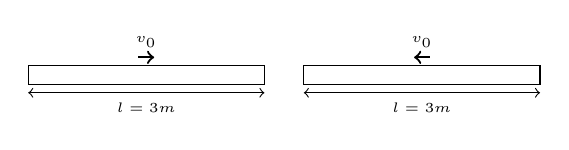
\begin{tikzpicture}
      \draw (0,0) rectangle (3,0.25);
      \draw[<->] (0,-0.1) -- (3,-0.1) node [midway, below] {\tiny $l=3m$};
      \draw[->,thick] (1.4,0.35) -- (1.6,0.35) node [midway, above] {\tiny $v_0$};
      \draw[<->] (3.5,-0.1) -- (6.5,-0.1) node [midway, below] {\tiny $l=3m$};
      \draw[<-,thick] (4.9,0.35) -- (5.1,0.35) node [midway, above] {\tiny $v_0$};
      \draw (3.5,0) rectangle (6.5,0.25);
    \end{tikzpicture}
  \end{block}
  %\pause
  \centering
  \begin{tikzpicture}[scale=.9]
\begin{groupplot}[group style={group size=2 by 2,
ylabels at=edge left, yticklabels at=edge left,horizontal sep=4.ex,
vertical sep=2ex,xticklabels at=edge bottom,xlabels at=edge bottom},
ymajorgrids=true,xmajorgrids=true,enlargelimits=0,xmin=0.,xmax=6.,xlabel=x (m),
axis on top,scale only axis,width=0.45\linewidth
]
\nextgroupplot[title={(a) time $t = 1.21\times 10^{-4} $ s.},ylabel=$\sigma (Pa)$,]
\addplot[Red,dashed,mark=none,very thick,mark size=3pt] coordinates{(0.0,-1.71821567874e-08) (0.122448979592,4.29553919686e-08) (0.244897959184,1.71821567874e-08) (0.367346938776,8.59107839372e-09) (0.489795918367,-1.71821567874e-08) (0.612244897959,-3.43643135749e-08) (0.734693877551,-2.57732351812e-08) (0.857142857143,0.0) (0.979591836735,0.0) (1.10204081633,-1.71821567874e-08) (1.22448979592,1.71821567874e-08) (1.34693877551,0.0) (1.4693877551,0.0) (1.59183673469,0.0) (1.71428571429,0.0) (1.83673469388,-10490.4174805) (1.95918367347,-180244.445801) (2.08163265306,-1426887.51221) (2.20408163265,-6905937.19482) (2.32653061224,-22447967.5293) (2.44897959184,-53339385.9863) (2.57142857143,-87870025.6348) (2.69387755102,-120363616.943) (2.81632653061,-112137222.29) (2.9387755102,-95318222.0459) (3.0612244898,-95318222.0459) (3.18367346939,-112137222.29) (3.30612244898,-120363616.943) (3.42857142857,-87870025.6348) (3.55102040816,-53339385.9863) (3.67346938776,-22447967.5293) (3.79591836735,-6905937.19482) (3.91836734694,-1426887.51221) (4.04081632653,-180244.445801) (4.16326530612,-10490.4174805) (4.28571428571,0.0) (4.40816326531,0.0) (4.5306122449,0.0) (4.65306122449,0.0) (4.77551020408,1.71821567874e-08) (4.89795918367,-1.71821567874e-08) (5.02040816327,0.0) (5.14285714286,0.0) (5.26530612245,0.0) (5.38775510204,0.0) (5.51020408163,0.0) (5.63265306122,0.0) (5.75510204082,0.0) (5.87755102041,0.0) (6.0,0.0) };
\addplot[Orange,densely dotted,mark=none,very thick,mark size=3pt] coordinates{(0.0,0.0) (0.0606060606061,0.0) (0.121212121212,0.0) (0.181818181818,0.0) (0.242424242424,0.0) (0.30303030303,0.0) (0.363636363636,0.0) (0.424242424242,0.0) (0.484848484848,0.0) (0.545454545455,0.0) (0.606060606061,-8.50429982409e-09) (0.666666666667,-8.50429982409e-09) (0.727272727273,0.0) (0.787878787879,0.0) (0.848484848485,0.0) (0.909090909091,0.0) (0.969696969697,8.50429982409e-09) (1.0303030303,8.50429982409e-09) (1.09090909091,0.0) (1.15151515152,0.0) (1.21212121212,0.0) (1.27272727273,0.0) (1.33333333333,0.0) (1.39393939394,0.0) (1.45454545455,0.0) (1.51515151515,0.0) (1.57575757576,0.0) (1.63636363636,0.0) (1.69696969697,0.0) (1.75757575758,0.0) (1.81818181818,-5499.27353859) (1.87878787879,-5499.27353859) (1.93939393939,-115492.194891) (2.0,-115492.194891) (2.06060606061,-1086898.89312) (2.12121212121,-1086898.89312) (2.18181818182,-6038592.01074) (2.24242424242,-6038592.01074) (2.30303030303,-21882501.2445) (2.36363636364,-21882501.2445) (2.42424242424,-54484376.3113) (2.48484848485,-54484376.3113) (2.54545454545,-94001361.7277) (2.60606060606,-94001361.7277) (2.66666666667,-117371180.654) (2.72727272727,-117371180.654) (2.78787878788,-111648218.334) (2.84848484848,-111648218.334) (2.90909090909,-93365879.3569) (2.9696969697,-93365879.3569) (3.0303030303,-93365879.3569) (3.09090909091,-93365879.3569) (3.15151515152,-111648218.334) (3.21212121212,-111648218.334) (3.27272727273,-117371180.654) (3.33333333333,-117371180.654) (3.39393939394,-94001361.7277) (3.45454545455,-94001361.7277) (3.51515151515,-54484376.3113) (3.57575757576,-54484376.3113) (3.63636363636,-21882501.2445) (3.69696969697,-21882501.2445) (3.75757575758,-6038592.01074) (3.81818181818,-6038592.01074) (3.87878787879,-1086898.89312) (3.93939393939,-1086898.89312) (4.0,-115492.194891) (4.06060606061,-115492.194891) (4.12121212121,-5499.2735386) (4.18181818182,-5499.2735386) (4.24242424242,-8.50429982409e-09) (4.30303030303,-8.50429982409e-09) (4.36363636364,1.70085996482e-08) (4.42424242424,1.70085996482e-08) (4.48484848485,-8.50429982409e-09) (4.54545454545,-8.50429982409e-09) (4.60606060606,0.0) (4.66666666667,0.0) (4.72727272727,0.0) (4.78787878788,0.0) (4.84848484848,0.0) (4.90909090909,0.0) (4.9696969697,0.0) (5.0303030303,0.0) (5.09090909091,0.0) (5.15151515152,0.0) (5.21212121212,0.0) (5.27272727273,0.0) (5.33333333333,0.0) (5.39393939394,0.0) (5.45454545455,0.0) (5.51515151515,0.0) (5.57575757576,0.0) (5.63636363636,0.0) (5.69696969697,0.0) (5.75757575758,0.0) (5.81818181818,0.0) (5.87878787879,0.0) (5.93939393939,0.0) (6.0,0.0) };
\addplot[Duck,solid,mark=*,thick,mark size=2pt] coordinates{(0.0,0.0) (0.0606060606061,0.0) (0.121212121212,0.0) (0.181818181818,0.0) (0.242424242424,0.0) (0.30303030303,0.0) (0.363636363636,-2.55128994723e-08) (0.424242424242,-2.55128994723e-08) (0.484848484848,-2.55128994723e-08) (0.545454545455,-2.55128994723e-08) (0.606060606061,-8.50429982409e-09) (0.666666666667,-8.50429982409e-09) (0.727272727273,-1.70085996482e-08) (0.787878787879,-1.70085996482e-08) (0.848484848485,1.70085996482e-08) (0.909090909091,1.70085996482e-08) (0.969696969697,1.70085996482e-08) (1.0303030303,1.70085996482e-08) (1.09090909091,8.50429982409e-09) (1.15151515152,8.50429982409e-09) (1.21212121212,2.55128994723e-08) (1.27272727273,2.55128994723e-08) (1.33333333333,8.50429982409e-09) (1.39393939394,8.50429982409e-09) (1.45454545455,0.0) (1.51515151515,0.0) (1.57575757576,-2.55128994723e-08) (1.63636363636,-2.55128994723e-08) (1.69696969697,-3.40171992963e-08) (1.75757575758,-3.40171992963e-08) (1.81818181818,-29361.1134112) (1.87878787879,-29361.1134112) (1.93939393939,-478765.91052) (2.0,-478765.91052) (2.06060606061,-3385772.94096) (2.12121212121,-3385772.94096) (2.18181818182,-13710104.1379) (2.24242424242,-13710104.1379) (2.30303030303,-35621767.9306) (2.36363636364,-35621767.9306) (2.42424242424,-64051116.4238) (2.48484848485,-64051116.4238) (2.54545454545,-86391746.7796) (2.60606060606,-86391746.7796) (2.66666666667,-96780453.3284) (2.72727272727,-96780453.3284) (2.78787878788,-99574824.0166) (2.84848484848,-99574824.0166) (2.90909090909,-99976087.4183) (2.9696969697,-99976087.4183) (3.0303030303,-99976087.4183) (3.09090909091,-99976087.4183) (3.15151515152,-99574824.0166) (3.21212121212,-99574824.0166) (3.27272727273,-96780453.3284) (3.33333333333,-96780453.3284) (3.39393939394,-86391746.7796) (3.45454545455,-86391746.7796) (3.51515151515,-64051116.4238) (3.57575757576,-64051116.4238) (3.63636363636,-35621767.9306) (3.69696969697,-35621767.9306) (3.75757575758,-13710104.1379) (3.81818181818,-13710104.1379) (3.87878787879,-3385772.94096) (3.93939393939,-3385772.94096) (4.0,-478765.91052) (4.06060606061,-478765.91052) (4.12121212121,-29361.1134111) (4.18181818182,-29361.1134111) (4.24242424242,0.0) (4.30303030303,0.0) (4.36363636364,3.40171992963e-08) (4.42424242424,3.40171992963e-08) (4.48484848485,-8.50429982409e-09) (4.54545454545,-8.50429982409e-09) (4.60606060606,0.0) (4.66666666667,0.0) (4.72727272727,0.0) (4.78787878788,0.0) (4.84848484848,0.0) (4.90909090909,0.0) (4.9696969697,0.0) (5.0303030303,0.0) (5.09090909091,0.0) (5.15151515152,0.0) (5.21212121212,0.0) (5.27272727273,0.0) (5.33333333333,0.0) (5.39393939394,0.0) (5.45454545455,0.0) (5.51515151515,0.0) (5.57575757576,0.0) (5.63636363636,0.0) (5.69696969697,0.0) (5.75757575758,0.0) (5.81818181818,0.0) (5.87878787879,0.0) (5.93939393939,0.0) (6.0,0.0) };
\addplot[Blue,solid,mark=none,very thick,mark size=3pt] coordinates{(0.0,2.20527643776e-23) (0.122448979592,-4.82139102982e-08) (0.244897959184,-3.61604327236e-08) (0.367346938776,2.41069551491e-08) (0.489795918367,-3.61604327236e-08) (0.612244897959,-2.41069551491e-08) (0.734693877551,1.20534775745e-08) (0.857142857143,-1.20534775745e-08) (0.979591836735,1.20534775745e-08) (1.10204081633,1.20534775745e-08) (1.22448979592,2.41069551491e-08) (1.34693877551,2.41069551491e-08) (1.4693877551,-6.30078982218e-24) (1.59183673469,-6.30078982218e-24) (1.71428571429,1.20534775745e-08) (1.83673469388,-2.41069551491e-08) (1.95918367347,0.0) (2.08163265306,0.0) (2.20408163265,1.57519745555e-23) (2.32653061224,1.57519745555e-23) (2.44897959184,-100000000.0) (2.57142857143,-100000000.0) (2.69387755102,-100000000.0) (2.81632653061,-100000000.0) (2.9387755102,-100000000.0) (3.0612244898,-100000000.0) (3.18367346939,-100000000.0) (3.30612244898,-100000000.0) (3.42857142857,-100000000.0) (3.55102040816,-100000000.0) (3.67346938776,-1.26015796444e-23) (3.79591836735,1.20534775745e-08) (3.91836734694,1.20534775745e-08) (4.04081632653,-3.61604327236e-08) (4.16326530612,1.41767770999e-23) (4.28571428571,-1.41767770999e-23) (4.40816326531,-2.41069551491e-08) (4.5306122449,-1.20534775745e-08) (4.65306122449,1.20534775745e-08) (4.77551020408,-1.89023694665e-23) (4.89795918367,-1.20534775745e-08) (5.02040816327,-2.41069551491e-08) (5.14285714286,3.61604327236e-08) (5.26530612245,-1.20534775745e-08) (5.38775510204,-1.89023694665e-23) (5.51020408163,2.41069551491e-08) (5.63265306122,-1.89023694665e-23) (5.75510204082,-1.20534775745e-08) (5.87755102041,2.41069551491e-08) (6.0,-1.57519745555e-23) };
\addplot[Purple,solid,mark=|,very thick,mark size=3pt] coordinates{(0.0,1.19548956657e-11) (0.0606060606061,-1.19548956657e-11) (0.121212121212,-9.04006220054e-09) (0.181818181818,-1.50668929485e-08) (0.242424242424,-2.01489535813e-08) (0.30303030303,-4.01184342914e-08) (0.363636363636,-3.98015720808e-08) (0.424242424242,-4.4572770941e-08) (0.484848484848,-3.05172621658e-08) (0.545454545455,-2.9750125707e-08) (0.606060606061,-1.89546709994e-08) (0.666666666667,-5.1522841497e-09) (0.727272727273,-1.17903779092e-08) (0.787878787879,-1.23165772399e-08) (0.848484848485,-2.54735836451e-08) (0.909090909091,1.36662849606e-09) (0.969696969697,3.64534656085e-08) (1.0303030303,2.38139222642e-08) (1.09090909091,2.4282772581e-08) (1.15151515152,2.39311377172e-08) (1.21212121212,1.22434109794e-08) (1.27272727273,1.18635441697e-08) (1.33333333333,1.25831714133e-08) (1.39393939394,1.15237837358e-08) (1.45454545455,2.73711934302e-08) (1.51515151515,2.08427168679e-08) (1.57575757576,9.62496696607e-09) (1.63636363636,1.4481988183e-08) (1.69696969697,2.10480996765e-08) (1.75757575758,1.51123330472e-08) (1.81818181818,-3666.24444723) (1.87878787879,-10998.7333417) (1.93939393939,-100618.042052) (2.0,-262747.518718) (2.06060606061,-1140066.23626) (2.12121212121,-2551162.98795) (2.18181818182,-6952185.18376) (2.24242424242,-13110550.493) (2.30303030303,-25132333.1147) (2.36363636364,-39370855.3165) (2.42424242424,-56894854.8287) (2.48484848485,-73865127.936) (2.54545454545,-86159824.58) (2.60606060606,-95498106.6287) (2.66666666667,-98513982.445) (2.72727272727,-100261419.266) (2.78787878788,-100094961.189) (2.84848484848,-100070640.631) (2.90909090909,-100007508.136) (2.9696969697,-99998390.4883) (3.0303030303,-99998390.4883) (3.09090909091,-100007508.136) (3.15151515152,-100070640.631) (3.21212121212,-100094961.189) (3.27272727273,-100261419.266) (3.33333333333,-98513982.445) (3.39393939394,-95498106.6287) (3.45454545455,-86159824.58) (3.51515151515,-73865127.936) (3.57575757576,-56894854.8287) (3.63636363636,-39370855.3165) (3.69696969697,-25132333.1147) (3.75757575758,-13110550.493) (3.81818181818,-6952185.18376) (3.87878787879,-2551162.98795) (3.93939393939,-1140066.23626) (4.0,-262747.518718) (4.06060606061,-100618.042052) (4.12121212121,-10998.7333417) (4.18181818182,-3666.24444723) (4.24242424242,6.0265548658e-09) (4.30303030303,6.02692270874e-09) (4.36363636364,2.0086063933e-09) (4.42424242424,-1.40620839678e-08) (4.48484848485,0.0) (4.54545454545,0.0) (4.60606060606,0.0) (4.66666666667,0.0) (4.72727272727,0.0) (4.78787878788,0.0) (4.84848484848,0.0) (4.90909090909,0.0) (4.9696969697,0.0) (5.0303030303,0.0) (5.09090909091,0.0) (5.15151515152,0.0) (5.21212121212,0.0) (5.27272727273,0.0) (5.33333333333,0.0) (5.39393939394,0.0) (5.45454545455,0.0) (5.51515151515,0.0) (5.57575757576,0.0) (5.63636363636,0.0) (5.69696969697,0.0) (5.75757575758,0.0) (5.81818181818,0.0) (5.87878787879,0.0) (5.93939393939,-6.02672729218e-09) (6.0,-6.02675028236e-09) };
\addplot[Green,only marks,mark=x,thick,mark size=3pt] coordinates{(0.0,-2.10935857555e-08) (0.0606060606061,-3.01336939364e-09) (0.121212121212,-2.50486330846e-08) (0.181818181818,-2.31652772136e-08) (0.242424242424,-1.40780851359e-08) (0.30303030303,-1.00288700132e-08) (0.363636363636,-4.37173981561e-08) (0.424242424242,-2.86034672912e-08) (0.484848484848,7.15675230988e-09) (0.545454545455,1.69502028392e-08) (0.606060606061,-4.36938562077e-08) (0.666666666667,-5.27339643886e-08) (0.727272727273,3.35237345042e-08) (0.787878787879,3.87971309431e-08) (0.848484848485,-1.48785113811e-08) (0.909090909091,-9.22844376801e-09) (0.969696969697,5.57002498855e-08) (1.0303030303,8.8941481009e-08) (1.09090909091,-5.9255084092e-08) (1.15151515152,-3.71727365043e-08) (1.21212121212,2.8956596517e-09) (1.27272727273,2.12112954974e-08) (1.33333333333,3.92679699108e-08) (1.39393939394,8.94594038736e-09) (1.45454545455,-2.01048239232e-08) (1.51515151515,-2.8109086375e-08) (1.57575757576,5.15568669692e-09) (1.63636363636,-5.15568669692e-09) (1.69696969697,1.90925201425e-08) (1.75757575758,5.0144350066e-09) (1.81818181818,-1.05467928777e-08) (1.87878787879,-1.35601622714e-08) (1.93939393939,-4.89672526466e-09) (2.0,-1.92102298844e-08) (2.06060606061,6.19153242599e-09) (2.12121212121,-6.19153242599e-09) (2.18181818182,-1.77741710328e-08) (2.24242424242,-3.04397392654e-08) (2.30303030303,1.76093773941e-08) (2.36363636364,6.49757775503e-09) (2.42424242424,-100000000.0) (2.48484848485,-100000000.0) (2.54545454545,-100000000.0) (2.60606060606,-100000000.0) (2.66666666667,-100000000.0) (2.72727272727,-100000000.0) (2.78787878788,-100000000.0) (2.84848484848,-100000000.0) (2.90909090909,-100000000.0) (2.9696969697,-100000000.0) (3.0303030303,-100000000.0) (3.09090909091,-100000000.0) (3.15151515152,-100000000.0) (3.21212121212,-100000000.0) (3.27272727273,-100000000.0) (3.33333333333,-100000000.0) (3.39393939394,-100000000.0) (3.45454545455,-100000000.0) (3.51515151515,-100000000.0) (3.57575757576,-100000000.0) (3.63636363636,0.0) (3.69696969697,0.0) (3.75757575758,0.0) (3.81818181818,0.0) (3.87878787879,0.0) (3.93939393939,0.0) (4.0,-6.02673878727e-09) (4.06060606061,-1.80802163618e-08) (4.12121212121,1.80802163618e-08) (4.18181818182,6.02673878727e-09) (4.24242424242,-1.64793638714e-10) (4.30303030303,-2.39421615104e-08) (4.36363636364,2.21058895361e-08) (4.42424242424,2.6108020762e-08) (4.48484848485,-1.10176318455e-08) (4.54545454545,-1.30893233036e-08) (4.60606060606,2.41069551491e-08) (4.66666666667,2.41069551491e-08) (4.72727272727,-2.41069551491e-08) (4.78787878788,-2.41069551491e-08) (4.84848484848,0.0) (4.90909090909,0.0) (4.9696969697,0.0) (5.0303030303,0.0) (5.09090909091,0.0) (5.15151515152,0.0) (5.21212121212,0.0) (5.27272727273,0.0) (5.33333333333,0.0) (5.39393939394,0.0) (5.45454545455,0.0) (5.51515151515,0.0) (5.57575757576,0.0) (5.63636363636,0.0) (5.69696969697,0.0) (5.75757575758,0.0) (5.81818181818,0.0) (5.87878787879,0.0) (5.93939393939,0.0) (6.0,0.0) };
\addplot[black,solid,mark=pentagone*,thin,mark size=3pt] coordinates{(0.0,-0.0) (0.122448979592,-0.0) (0.244897959184,-0.0) (0.367346938776,-0.0) (0.489795918367,-0.0) (0.612244897959,-0.0) (0.734693877551,-0.0) (0.857142857143,-0.0) (0.979591836735,-0.0) (1.10204081633,-0.0) (1.22448979592,-0.0) (1.34693877551,-0.0) (1.4693877551,-0.0) (1.59183673469,-0.0) (1.71428571429,-0.0) (1.83673469388,-0.0) (1.95918367347,-0.0) (2.08163265306,-0.0) (2.20408163265,-0.0) (2.32653061224,-0.0) (2.44897959184,-100000000.0) (2.57142857143,-100000000.0) (2.69387755102,-100000000.0) (2.81632653061,-100000000.0) (2.9387755102,-100000000.0) (3.0612244898,-100000000.0) (3.18367346939,-100000000.0) (3.30612244898,-100000000.0) (3.42857142857,-100000000.0) (3.55102040816,-100000000.0) (3.67346938776,-0.0) (3.79591836735,-0.0) (3.91836734694,-0.0) (4.04081632653,-0.0) (4.16326530612,-0.0) (4.28571428571,-0.0) (4.40816326531,-0.0) (4.5306122449,-0.0) (4.65306122449,-0.0) (4.77551020408,-0.0) (4.89795918367,-0.0) (5.02040816327,-0.0) (5.14285714286,-0.0) (5.26530612245,-0.0) (5.38775510204,-0.0) (5.51020408163,-0.0) (5.63265306122,-0.0) (5.75510204082,-0.0) (5.87755102041,-0.0) (6.0,-0.0) };
\nextgroupplot[title={(b) time $t = 4.84\times 10^{-4} $ s.},]
\addplot[Red,dashed,mark=none,very thick,mark size=3pt] coordinates{(0.0,-8.59107839372e-09) (0.122448979592,4.29553919686e-08) (0.244897959184,2.57732351812e-08) (0.367346938776,8.59107839372e-09) (0.489795918367,-8.59107839372e-09) (0.612244897959,-1.23054636115) (0.734693877551,-40.5516402702) (0.857142857143,-640.213875183) (0.979591836735,-6438.55873936) (1.10204081633,-46257.8011138) (1.22448979592,-252333.895514) (1.34693877551,-1084103.88038) (1.4693877551,-3755013.24106) (1.59183673469,-10642636.9901) (1.71428571429,-24916947.9583) (1.83673469388,-48387367.3518) (1.95918367347,-78275857.836) (2.08163265306,-105019368.728) (2.20408163265,-119223316.597) (2.32653061224,-113889153.316) (2.44897959184,-103439986.404) (2.57142857143,-92963963.4978) (2.69387755102,-96202736.2231) (2.81632653061,-98859035.7487) (2.9387755102,-103034799.977) (3.0612244898,-103034799.977) (3.18367346939,-98859035.7487) (3.30612244898,-96202736.2231) (3.42857142857,-92963963.4978) (3.55102040816,-103439986.404) (3.67346938776,-113889153.316) (3.79591836735,-119223316.597) (3.91836734694,-105019368.728) (4.04081632653,-78275857.836) (4.16326530612,-48387367.3518) (4.28571428571,-24916947.9583) (4.40816326531,-10642636.9901) (4.5306122449,-3755013.24106) (4.65306122449,-1084103.88038) (4.77551020408,-252333.895514) (4.89795918367,-46257.8011138) (5.02040816327,-6438.55873932) (5.14285714286,-640.213875175) (5.26530612245,-40.5516402702) (5.38775510204,-1.23054632679) (5.51020408163,0.0) (5.63265306122,0.0) (5.75510204082,0.0) (5.87755102041,0.0) (6.0,0.0) };
\addplot[Orange,densely dotted,mark=none,very thick,mark size=3pt] coordinates{(0.0,0.0) (0.0606060606061,0.0) (0.121212121212,0.0) (0.181818181818,0.0) (0.242424242424,0.0) (0.30303030303,0.0) (0.363636363636,0.0) (0.424242424242,0.0) (0.484848484848,0.0) (0.545454545455,0.0) (0.606060606061,-0.302430335559) (0.666666666667,-0.302430335559) (0.727272727273,-12.3996438685) (0.787878787879,-12.3996438685) (0.848484848485,-240.230497765) (0.909090909091,-240.230497765) (0.969696969697,-2921.77951372) (1.0303030303,-2921.77951372) (1.09090909091,-24993.4810877) (1.15151515152,-24993.4810877) (1.21212121212,-159637.896304) (1.27272727273,-159637.896304) (1.33333333333,-788716.389772) (1.39393939394,-788716.389772) (1.45454545455,-3080624.98423) (1.51515151515,-3080624.98423) (1.57575757576,-9638116.18636) (1.63636363636,-9638116.18636) (1.69696969697,-24323655.3377) (1.75757575758,-24323655.3377) (1.81818181818,-49636559.9635) (1.87878787879,-49636559.9635) (1.93939393939,-81867011.1376) (2.0,-81867011.1376) (2.06060606061,-109111634.24) (2.12121212121,-109111634.24) (2.18181818182,-118687950.99) (2.24242424242,-118687950.99) (2.30303030303,-110105828.793) (2.36363636364,-110105828.793) (2.42424242424,-97435608.9991) (2.48484848485,-97435608.9991) (2.54545454545,-94244104.916) (2.60606060606,-94244104.916) (2.66666666667,-99081654.2889) (2.72727272727,-99081654.2889) (2.78787878788,-101740412.886) (2.84848484848,-101740412.886) (2.90909090909,-100070314.798) (2.9696969697,-100070314.798) (3.0303030303,-100070314.798) (3.09090909091,-100070314.798) (3.15151515152,-101740412.886) (3.21212121212,-101740412.886) (3.27272727273,-99081654.2889) (3.33333333333,-99081654.2889) (3.39393939394,-94244104.916) (3.45454545455,-94244104.916) (3.51515151515,-97435608.9991) (3.57575757576,-97435608.9991) (3.63636363636,-110105828.793) (3.69696969697,-110105828.793) (3.75757575758,-118687950.99) (3.81818181818,-118687950.99) (3.87878787879,-109111634.24) (3.93939393939,-109111634.24) (4.0,-81867011.1376) (4.06060606061,-81867011.1376) (4.12121212121,-49636559.9635) (4.18181818182,-49636559.9635) (4.24242424242,-24323655.3377) (4.30303030303,-24323655.3377) (4.36363636364,-9638116.18636) (4.42424242424,-9638116.18636) (4.48484848485,-3080624.98423) (4.54545454545,-3080624.98423) (4.60606060606,-788716.389772) (4.66666666667,-788716.389772) (4.72727272727,-159637.896304) (4.78787878788,-159637.896304) (4.84848484848,-24993.4810877) (4.90909090909,-24993.4810877) (4.9696969697,-2921.7795137) (5.0303030303,-2921.7795137) (5.09090909091,-240.230497756) (5.15151515152,-240.230497756) (5.21212121212,-12.3996438685) (5.27272727273,-12.3996438685) (5.33333333333,-0.302430344063) (5.39393939394,-0.302430344063) (5.45454545455,0.0) (5.51515151515,0.0) (5.57575757576,0.0) (5.63636363636,0.0) (5.69696969697,0.0) (5.75757575758,0.0) (5.81818181818,0.0) (5.87878787879,0.0) (5.93939393939,0.0) (6.0,0.0) };
\addplot[Duck,solid,mark=*,thick,mark size=2pt] coordinates{(0.0,-8.50429982409e-09) (0.0606060606061,-8.50429982409e-09) (0.121212121212,-2.55128994723e-08) (0.181818181818,-2.55128994723e-08) (0.242424242424,-1.70085996482e-08) (0.30303030303,-1.70085996482e-08) (0.363636363636,-5.10257989445e-08) (0.424242424242,-5.10257989445e-08) (0.484848484848,-3.40171992963e-08) (0.545454545455,-3.40171992963e-08) (0.606060606061,-7.54315610416) (0.666666666667,-7.54315610416) (0.727272727273,-243.074356172) (0.787878787879,-243.074356172) (0.848484848485,-3634.66708743) (0.909090909091,-3634.66708743) (0.969696969697,-33492.7067527) (1.0303030303,-33492.7067527) (1.09090909091,-213117.914955) (1.15151515152,-213117.914955) (1.21212121212,-995090.547212) (1.27272727273,-995090.547212) (1.33333333333,-3540220.94427) (1.39393939394,-3540220.94427) (1.45454545455,-9852354.5249) (1.51515151515,-9852354.5249) (1.57575757576,-21906072.5461) (1.63636363636,-21906072.5461) (1.69696969697,-39711055.8831) (1.75757575758,-39711055.8831) (1.81818181818,-60065449.8718) (1.87878787879,-60065449.8718) (1.93939393939,-78032993.3013) (2.0,-78032993.3013) (2.06060606061,-90231435.0995) (2.12121212121,-90231435.0995) (2.18181818182,-96567889.7944) (2.24242424242,-96567889.7944) (2.30303030303,-99068409.7758) (2.36363636364,-99068409.7758) (2.42424242424,-99809735.7536) (2.48484848485,-99809735.7536) (2.54545454545,-99971826.9969) (2.60606060606,-99971826.9969) (2.66666666667,-99997149.6439) (2.72727272727,-99997149.6439) (2.78787878788,-99999824.5348) (2.84848484848,-99999824.5348) (2.90909090909,-99999994.876) (2.9696969697,-99999994.876) (3.0303030303,-99999994.876) (3.09090909091,-99999994.876) (3.15151515152,-99999824.5348) (3.21212121212,-99999824.5348) (3.27272727273,-99997149.6439) (3.33333333333,-99997149.6439) (3.39393939394,-99971826.9969) (3.45454545455,-99971826.9969) (3.51515151515,-99809735.7536) (3.57575757576,-99809735.7536) (3.63636363636,-99068409.7758) (3.69696969697,-99068409.7758) (3.75757575758,-96567889.7944) (3.81818181818,-96567889.7944) (3.87878787879,-90231435.0995) (3.93939393939,-90231435.0995) (4.0,-78032993.3013) (4.06060606061,-78032993.3013) (4.12121212121,-60065449.8718) (4.18181818182,-60065449.8718) (4.24242424242,-39711055.8831) (4.30303030303,-39711055.8831) (4.36363636364,-21906072.5461) (4.42424242424,-21906072.5461) (4.48484848485,-9852354.5249) (4.54545454545,-9852354.5249) (4.60606060606,-3540220.94427) (4.66666666667,-3540220.94427) (4.72727272727,-995090.547212) (4.78787878788,-995090.547212) (4.84848484848,-213117.914955) (4.90909090909,-213117.914955) (4.9696969697,-33492.7067527) (5.0303030303,-33492.7067527) (5.09090909091,-3634.66708747) (5.15151515152,-3634.66708747) (5.21212121212,-243.074356181) (5.27272727273,-243.074356181) (5.33333333333,-7.54315609566) (5.39393939394,-7.54315609566) (5.45454545455,0.0) (5.51515151515,0.0) (5.57575757576,0.0) (5.63636363636,0.0) (5.69696969697,0.0) (5.75757575758,0.0) (5.81818181818,0.0) (5.87878787879,0.0) (5.93939393939,0.0) (6.0,0.0) };
\addplot[Blue,solid,mark=none,very thick,mark size=3pt] coordinates{(0.0,1.89023694665e-23) (0.122448979592,6.30078982218e-23) (0.244897959184,-2.20527643776e-23) (0.367346938776,1.08481298171e-07) (0.489795918367,-6.02673878727e-08) (0.612244897959,-3.78047389331e-23) (0.734693877551,-2.41069551491e-08) (0.857142857143,-1.20534775745e-08) (0.979591836735,3.61604327236e-08) (1.10204081633,-1.20534775745e-08) (1.22448979592,3.61604327236e-08) (1.34693877551,-3.15039491109e-24) (1.4693877551,1.20534775745e-08) (1.59183673469,-6.30078982218e-24) (1.71428571429,2.41069551491e-08) (1.83673469388,-100000000.0) (1.95918367347,-100000000.0) (2.08163265306,-100000000.0) (2.20408163265,-100000000.0) (2.32653061224,-100000000.0) (2.44897959184,-100000000.0) (2.57142857143,-100000000.0) (2.69387755102,-100000000.0) (2.81632653061,-100000000.0) (2.9387755102,-100000000.0) (3.0612244898,-100000000.0) (3.18367346939,-100000000.0) (3.30612244898,-100000000.0) (3.42857142857,-100000000.0) (3.55102040816,-100000000.0) (3.67346938776,-100000000.0) (3.79591836735,-100000000.0) (3.91836734694,-100000000.0) (4.04081632653,-100000000.0) (4.16326530612,-100000000.0) (4.28571428571,1.20534775745e-08) (4.40816326531,-3.61604327236e-08) (4.5306122449,-6.30078982218e-24) (4.65306122449,-2.41069551491e-08) (4.77551020408,-1.20534775745e-08) (4.89795918367,-4.82139102982e-08) (5.02040816327,-3.30791465665e-23) (5.14285714286,2.41069551491e-08) (5.26530612245,-4.82139102982e-08) (5.38775510204,2.41069551491e-08) (5.51020408163,-3.15039491109e-23) (5.63265306122,-3.61604327236e-08) (5.75510204082,2.41069551491e-08) (5.87755102041,3.61604327236e-08) (6.0,-1.20534775745e-08) };
\addplot[Purple,solid,mark=|,very thick,mark size=3pt] coordinates{(0.0,-6.62623071053e-10) (0.0606060606061,-1.13908545035e-08) (0.121212121212,-1.03251991157e-08) (0.181818181818,-2.58352336079e-08) (0.242424242424,-5.14381821174e-08) (0.30303030303,-4.4989638479e-08) (0.363636363636,-5.34390135805e-08) (0.424242424242,-5.50422845904e-08) (0.484848484848,-2.21025908105e-08) (0.545454545455,-3.81647970622e-08) (0.606060606061,-0.201620272159) (0.666666666667,-0.604860699987) (0.727272727273,-10.6858719382) (0.787878787879,-29.9070000639) (0.848484848485,-256.986134699) (0.909090909091,-668.206763393) (0.969696969697,-3715.07114041) (1.0303030303,-8933.82287809) (1.09090909091,-36066.6707163) (1.15151515152,-79819.6254771) (1.21212121212,-248965.8763) (1.27272727273,-504422.520742) (1.33333333333,-1263261.9825) (1.39393939394,-2330406.84983) (1.45454545455,-4810891.93605) (1.51515151515,-8037941.25365) (1.57575757576,-13953612.4785) (1.63636363636,-21022005.3552) (1.69696969697,-31228050.0112) (1.75757575758,-42338748.4528) (1.81818181818,-54831068.3252) (1.87878787879,-67114743.6608) (1.93939393939,-77590809.6787) (2.0,-86813439.423) (2.06060606061,-92463242.0658) (2.12121212121,-96885420.8686) (2.18181818182,-98592164.6111) (2.24242424242,-99785509.2556) (2.30303030303,-99950031.6158) (2.36363636364,-100067351.927) (2.42424242424,-100025492.446) (2.48484848485,-100011084.154) (2.54545454545,-100002494.767) (2.60606060606,-99999559.9552) (2.66666666667,-99999874.1387) (2.72727272727,-99999912.159) (2.78787878788,-99999990.2886) (2.84848484848,-100000001.919) (2.90909090909,-100000000.164) (2.9696969697,-100000000.078) (3.0303030303,-100000000.078) (3.09090909091,-100000000.164) (3.15151515152,-100000001.919) (3.21212121212,-99999990.2886) (3.27272727273,-99999912.159) (3.33333333333,-99999874.1387) (3.39393939394,-99999559.9552) (3.45454545455,-100002494.767) (3.51515151515,-100011084.154) (3.57575757576,-100025492.446) (3.63636363636,-100067351.927) (3.69696969697,-99950031.6158) (3.75757575758,-99785509.2556) (3.81818181818,-98592164.6111) (3.87878787879,-96885420.8686) (3.93939393939,-92463242.0658) (4.0,-86813439.423) (4.06060606061,-77590809.6787) (4.12121212121,-67114743.6608) (4.18181818182,-54831068.3252) (4.24242424242,-42338748.4528) (4.30303030303,-31228050.0112) (4.36363636364,-21022005.3552) (4.42424242424,-13953612.4785) (4.48484848485,-8037941.25365) (4.54545454545,-4810891.93605) (4.60606060606,-2330406.84983) (4.66666666667,-1263261.9825) (4.72727272727,-504422.520742) (4.78787878788,-248965.8763) (4.84848484848,-79819.6254771) (4.90909090909,-36066.6707163) (4.9696969697,-8933.82287811) (5.0303030303,-3715.07114043) (5.09090909091,-668.206763402) (5.15151515152,-256.986134702) (5.21212121212,-29.9070000726) (5.27272727273,-10.6858719415) (5.33333333333,-0.604860674869) (5.39393939394,-0.201620224956) (5.45454545455,0.0) (5.51515151515,0.0) (5.57575757576,0.0) (5.63636363636,0.0) (5.69696969697,0.0) (5.75757575758,0.0) (5.81818181818,0.0) (5.87878787879,0.0) (5.93939393939,-6.02673878726e-09) (6.0,-6.02673878728e-09) };
\addplot[Green,only marks,mark=x,thick,mark size=3pt] coordinates{(0.0,-4.24785031222e-08) (0.0606060606061,-5.39493174741e-08) (0.121212121212,4.17860387809e-08) (0.181818181818,3.05348266663e-08) (0.242424242424,-1.08312734142e-08) (0.30303030303,1.08312734142e-08) (0.363636363636,-1.37558777075e-08) (0.424242424242,-1.03510774416e-08) (0.484848484848,-6.55691082182e-08) (0.545454545455,-5.49656675272e-08) (0.606060606061,-4.3242145073e-08) (0.666666666667,-2.90787203742e-08) (0.727272727273,-3.72459372501e-08) (0.787878787879,-3.50749281972e-08) (0.848484848485,-3.29863159637e-09) (0.909090909091,-2.08083235527e-08) (0.969696969697,1.35203892531e-08) (1.0303030303,1.0586565896e-08) (1.09090909091,1.42527645537e-09) (1.15151515152,-1.42527645537e-09) (1.21212121212,-4.952752343e-09) (1.27272727273,4.952752343e-09) (1.33333333333,4.19430157571e-08) (1.39393939394,3.03778496901e-08) (1.45454545455,3.00669764225e-08) (1.51515151515,4.22538890248e-08) (1.57575757576,-1.21426105178e-08) (1.63636363636,-1.19643446313e-08) (1.69696969697,1.70747866461e-08) (1.75757575758,3.1139123652e-08) (1.81818181818,-100000000.0) (1.87878787879,-100000000.0) (1.93939393939,-100000000.0) (2.0,-100000000.0) (2.06060606061,-100000000.0) (2.12121212121,-100000000.0) (2.18181818182,-100000000.0) (2.24242424242,-100000000.0) (2.30303030303,-100000000.0) (2.36363636364,-100000000.0) (2.42424242424,-100000000.0) (2.48484848485,-100000000.0) (2.54545454545,-100000000.0) (2.60606060606,-100000000.0) (2.66666666667,-100000000.0) (2.72727272727,-100000000.0) (2.78787878788,-100000000.0) (2.84848484848,-100000000.0) (2.90909090909,-100000000.0) (2.9696969697,-100000000.0) (3.0303030303,-100000000.0) (3.09090909091,-100000000.0) (3.15151515152,-100000000.0) (3.21212121212,-100000000.0) (3.27272727273,-100000000.0) (3.33333333333,-100000000.0) (3.39393939394,-100000000.0) (3.45454545455,-100000000.0) (3.51515151515,-100000000.0) (3.57575757576,-100000000.0) (3.63636363636,-100000000.0) (3.69696969697,-100000000.0) (3.75757575758,-100000000.0) (3.81818181818,-100000000.0) (3.87878787879,-100000000.0) (3.93939393939,-100000000.0) (4.0,-100000000.0) (4.06060606061,-100000000.0) (4.12121212121,-100000000.0) (4.18181818182,-100000000.0) (4.24242424242,-4.81448937659e-09) (4.30303030303,4.81448937659e-09) (4.36363636364,-1.4144710689e-09) (4.42424242424,1.4144710689e-09) (4.48484848485,1.2195740833e-08) (4.54545454545,1.19112143161e-08) (4.60606060606,-3.0110151988e-08) (4.66666666667,-4.22107134593e-08) (4.72727272727,-6.28570021954e-09) (4.78787878788,-1.78212549295e-08) (4.84848484848,8.92239843897e-09) (4.90909090909,1.51845567101e-08) (4.9696969697,-4.2375507098e-09) (5.0303030303,4.2375507098e-09) (5.09090909091,-1.35601622714e-08) (5.15151515152,-1.05467928777e-08) (5.21212121212,1.20534775745e-08) (5.27272727273,3.61604327236e-08) (5.33333333333,-4.21871715109e-08) (5.39393939394,-3.01336939364e-08) (5.45454545455,0.0) (5.51515151515,0.0) (5.57575757576,0.0) (5.63636363636,0.0) (5.69696969697,0.0) (5.75757575758,0.0) (5.81818181818,0.0) (5.87878787879,0.0) (5.93939393939,0.0) (6.0,0.0) };
\addplot[black,solid,mark=pentagone*,thin,mark size=3pt] coordinates{(0.0,-0.0) (0.122448979592,-0.0) (0.244897959184,-0.0) (0.367346938776,-0.0) (0.489795918367,-0.0) (0.612244897959,-0.0) (0.734693877551,-0.0) (0.857142857143,-0.0) (0.979591836735,-0.0) (1.10204081633,-0.0) (1.22448979592,-0.0) (1.34693877551,-0.0) (1.4693877551,-0.0) (1.59183673469,-0.0) (1.71428571429,-0.0) (1.83673469388,-100000000.0) (1.95918367347,-100000000.0) (2.08163265306,-100000000.0) (2.20408163265,-100000000.0) (2.32653061224,-100000000.0) (2.44897959184,-100000000.0) (2.57142857143,-100000000.0) (2.69387755102,-100000000.0) (2.81632653061,-100000000.0) (2.9387755102,-100000000.0) (3.0612244898,-100000000.0) (3.18367346939,-100000000.0) (3.30612244898,-100000000.0) (3.42857142857,-100000000.0) (3.55102040816,-100000000.0) (3.67346938776,-100000000.0) (3.79591836735,-100000000.0) (3.91836734694,-100000000.0) (4.04081632653,-100000000.0) (4.16326530612,-100000000.0) (4.28571428571,-0.0) (4.40816326531,-0.0) (4.5306122449,-0.0) (4.65306122449,-0.0) (4.77551020408,-0.0) (4.89795918367,-0.0) (5.02040816327,-0.0) (5.14285714286,-0.0) (5.26530612245,-0.0) (5.38775510204,-0.0) (5.51020408163,-0.0) (5.63265306122,-0.0) (5.75510204082,-0.0) (5.87755102041,-0.0) (6.0,-0.0) };
\nextgroupplot[ylabel=v (m/s),]
\addplot[Red,dashed,mark=none,very thick,mark size=3pt] coordinates{(0.0,2.53184841771) (0.122448979592,2.53184841771) (0.244897959184,2.53184841771) (0.367346938776,2.53184841771) (0.489795918367,2.53184841771) (0.612244897959,2.53184841771) (0.734693877551,2.53184841771) (0.857142857143,2.53184841771) (0.979591836735,2.53184841771) (1.10204081633,2.53184841771) (1.22448979592,2.53184841771) (1.34693877551,2.53184841771) (1.4693877551,2.53184841771) (1.59183673469,2.53184841771) (1.71428571429,2.53184841771) (1.83673469388,2.53168422771) (1.95918367347,2.52888333949) (2.08163265306,2.50699777845) (2.20408163265,2.40545109318) (2.32653061224,2.08436306275) (2.44897959184,1.45719589947) (2.57142857143,0.368133294256) (2.69387755102,0.0385943080031) (2.81632653061,-0.906077680431) (2.9387755102,0.154976042597) (3.0612244898,-0.154976042597) (3.18367346939,0.906077680431) (3.30612244898,-0.0385943080031) (3.42857142857,-0.368133294256) (3.55102040816,-1.45719589947) (3.67346938776,-2.08436306275) (3.79591836735,-2.40545109318) (3.91836734694,-2.50699777845) (4.04081632653,-2.52888333949) (4.16326530612,-2.53168422771) (4.28571428571,-2.53184841771) (4.40816326531,-2.53184841771) (4.5306122449,-2.53184841771) (4.65306122449,-2.53184841771) (4.77551020408,-2.53184841771) (4.89795918367,-2.53184841771) (5.02040816327,-2.53184841771) (5.14285714286,-2.53184841771) (5.26530612245,-2.53184841771) (5.38775510204,-2.53184841771) (5.51020408163,-2.53184841771) (5.63265306122,-2.53184841771) (5.75510204082,-2.53184841771) (5.87755102041,-2.53184841771) (6.0,-2.53184841771) };
\addplot[Orange,densely dotted,mark=none,very thick,mark size=3pt] coordinates{(0.0,2.53184841771) (0.0606060606061,2.53184841771) (0.121212121212,2.53184841771) (0.181818181818,2.53184841771) (0.242424242424,2.53184841771) (0.30303030303,2.53184841771) (0.363636363636,2.53184841771) (0.424242424242,2.53184841771) (0.484848484848,2.53184841771) (0.545454545455,2.53184841771) (0.606060606061,2.53184841771) (0.666666666667,2.53184841771) (0.727272727273,2.53184841771) (0.787878787879,2.53184841771) (0.848484848485,2.53184841771) (0.909090909091,2.53184841771) (0.969696969697,2.53184841771) (1.0303030303,2.53184841771) (1.09090909091,2.53184841771) (1.15151515152,2.53184841771) (1.21212121212,2.53184841771) (1.27272727273,2.53184841771) (1.33333333333,2.53184841771) (1.39393939394,2.53184841771) (1.45454545455,2.53184841771) (1.51515151515,2.53184841771) (1.57575757576,2.53184841771) (1.63636363636,2.53184841771) (1.69696969697,2.53184841771) (1.75757575758,2.53184841771) (1.81818181818,2.53180200348) (1.87878787879,2.53170917501) (1.93939393939,2.53075014243) (2.0,2.52892490574) (2.06060606061,2.52011291678) (2.12121212121,2.50431417554) (2.18181818182,2.45734572485) (2.24242424242,2.37920756473) (2.30303030303,2.21852587251) (2.36363636364,1.97530064819) (2.42424242424,1.62562122327) (2.48484848485,1.16948759776) (2.54545454545,0.652158035596) (2.60606060606,0.0736325367928) (2.66666666667,-0.209593400584) (2.72727272727,-0.197519776535) (2.78787878788,-0.41340730943) (2.84848484848,-0.857255999272) (2.90909090909,-0.176423153717) (2.9696969697,1.62909122723) (3.0303030303,-1.62909122723) (3.09090909091,0.176423153717) (3.15151515152,0.857255999272) (3.21212121212,0.41340730943) (3.27272727273,0.197519776535) (3.33333333333,0.209593400584) (3.39393939394,-0.0736325367928) (3.45454545455,-0.652158035596) (3.51515151515,-1.16948759776) (3.57575757576,-1.62562122327) (3.63636363636,-1.97530064819) (3.69696969697,-2.21852587251) (3.75757575758,-2.37920756473) (3.81818181818,-2.45734572485) (3.87878787879,-2.50431417554) (3.93939393939,-2.52011291678) (4.0,-2.52892490574) (4.06060606061,-2.53075014243) (4.12121212121,-2.53170917501) (4.18181818182,-2.53180200348) (4.24242424242,-2.53184841771) (4.30303030303,-2.53184841771) (4.36363636364,-2.53184841771) (4.42424242424,-2.53184841771) (4.48484848485,-2.53184841771) (4.54545454545,-2.53184841771) (4.60606060606,-2.53184841771) (4.66666666667,-2.53184841771) (4.72727272727,-2.53184841771) (4.78787878788,-2.53184841771) (4.84848484848,-2.53184841771) (4.90909090909,-2.53184841771) (4.9696969697,-2.53184841771) (5.0303030303,-2.53184841771) (5.09090909091,-2.53184841771) (5.15151515152,-2.53184841771) (5.21212121212,-2.53184841771) (5.27272727273,-2.53184841771) (5.33333333333,-2.53184841771) (5.39393939394,-2.53184841771) (5.45454545455,-2.53184841771) (5.51515151515,-2.53184841771) (5.57575757576,-2.53184841771) (5.63636363636,-2.53184841771) (5.69696969697,-2.53184841771) (5.75757575758,-2.53184841771) (5.81818181818,-2.53184841771) (5.87878787879,-2.53184841771) (5.93939393939,-2.53184841771) (6.0,-2.53184841771) };
\addplot[Duck,solid,mark=*,thick,mark size=2pt] coordinates{(0.0,2.53184841771) (0.0606060606061,2.53184841771) (0.121212121212,2.53184841771) (0.181818181818,2.53184841771) (0.242424242424,2.53184841771) (0.30303030303,2.53184841771) (0.363636363636,2.53184841771) (0.424242424242,2.53184841771) (0.484848484848,2.53184841771) (0.545454545455,2.53184841771) (0.606060606061,2.53184841771) (0.666666666667,2.53184841771) (0.727272727273,2.53184841771) (0.787878787879,2.53184841771) (0.848484848485,2.53184841771) (0.909090909091,2.53184841771) (0.969696969697,2.53184841771) (1.0303030303,2.53184841771) (1.09090909091,2.53184841771) (1.15151515152,2.53184841771) (1.21212121212,2.53184841771) (1.27272727273,2.53184841771) (1.33333333333,2.53184841771) (1.39393939394,2.53184841771) (1.45454545455,2.53184841771) (1.51515151515,2.53184841771) (1.57575757576,2.53184841771) (1.63636363636,2.53184841771) (1.69696969697,2.53184841771) (1.75757575758,2.53184841771) (1.81818181818,2.53147672827) (1.87878787879,2.53073334938) (1.93939393939,2.52515042224) (2.0,2.51472794685) (2.06060606061,2.47915629191) (2.12121212121,2.41843545742) (2.18181818182,2.29318461062) (2.24242424242,2.10340375152) (2.30303030303,1.83698560404) (2.36363636364,1.49393016818) (2.42424242424,1.14155493551) (2.48484848485,0.779859906029) (2.54545454545,0.490899655057) (2.60606060606,0.274674182594) (2.66666666667,0.131308307876) (2.72727272727,0.0608020309012) (2.78787878788,0.0195497010067) (2.84848484848,0.00755131819221) (2.90909090909,0.00116409508873) (2.9696969697,0.000388031696242) (3.0303030303,-0.000388031696245) (3.09090909091,-0.00116409508873) (3.15151515152,-0.00755131819221) (3.21212121212,-0.0195497010067) (3.27272727273,-0.0608020309012) (3.33333333333,-0.131308307876) (3.39393939394,-0.274674182594) (3.45454545455,-0.490899655057) (3.51515151515,-0.779859906029) (3.57575757576,-1.14155493551) (3.63636363636,-1.49393016818) (3.69696969697,-1.83698560404) (3.75757575758,-2.10340375152) (3.81818181818,-2.29318461062) (3.87878787879,-2.41843545742) (3.93939393939,-2.47915629191) (4.0,-2.51472794685) (4.06060606061,-2.52515042224) (4.12121212121,-2.53073334938) (4.18181818182,-2.53147672827) (4.24242424242,-2.53184841771) (4.30303030303,-2.53184841771) (4.36363636364,-2.53184841771) (4.42424242424,-2.53184841771) (4.48484848485,-2.53184841771) (4.54545454545,-2.53184841771) (4.60606060606,-2.53184841771) (4.66666666667,-2.53184841771) (4.72727272727,-2.53184841771) (4.78787878788,-2.53184841771) (4.84848484848,-2.53184841771) (4.90909090909,-2.53184841771) (4.9696969697,-2.53184841771) (5.0303030303,-2.53184841771) (5.09090909091,-2.53184841771) (5.15151515152,-2.53184841771) (5.21212121212,-2.53184841771) (5.27272727273,-2.53184841771) (5.33333333333,-2.53184841771) (5.39393939394,-2.53184841771) (5.45454545455,-2.53184841771) (5.51515151515,-2.53184841771) (5.57575757576,-2.53184841771) (5.63636363636,-2.53184841771) (5.69696969697,-2.53184841771) (5.75757575758,-2.53184841771) (5.81818181818,-2.53184841771) (5.87878787879,-2.53184841771) (5.93939393939,-2.53184841771) (6.0,-2.53184841771) };
\addplot[Blue,solid,mark=none,very thick,mark size=3pt] coordinates{(0.0,2.53184841771) (0.122448979592,2.53184841771) (0.244897959184,2.53184841771) (0.367346938776,2.53184841771) (0.489795918367,2.53184841771) (0.612244897959,2.53184841771) (0.734693877551,2.53184841771) (0.857142857143,2.53184841771) (0.979591836735,2.53184841771) (1.10204081633,2.53184841771) (1.22448979592,2.53184841771) (1.34693877551,2.53184841771) (1.4693877551,2.53184841771) (1.59183673469,2.53184841771) (1.71428571429,2.53184841771) (1.83673469388,2.53184841771) (1.95918367347,2.53184841771) (2.08163265306,2.53184841771) (2.20408163265,2.53184841771) (2.32653061224,2.53184841771) (2.44897959184,0.0) (2.57142857143,-1.13182444172e-15) (2.69387755102,3.77274813907e-16) (2.81632653061,-3.94430452611e-31) (2.9387755102,7.54549627813e-16) (3.0612244898,-1.13182444172e-15) (3.18367346939,3.77274813907e-16) (3.30612244898,3.77274813907e-16) (3.42857142857,7.54549627813e-16) (3.55102040816,2.22044604925e-16) (3.67346938776,-2.53184841771) (3.79591836735,-2.53184841771) (3.91836734694,-2.53184841771) (4.04081632653,-2.53184841771) (4.16326530612,-2.53184841771) (4.28571428571,-2.53184841771) (4.40816326531,-2.53184841771) (4.5306122449,-2.53184841771) (4.65306122449,-2.53184841771) (4.77551020408,-2.53184841771) (4.89795918367,-2.53184841771) (5.02040816327,-2.53184841771) (5.14285714286,-2.53184841771) (5.26530612245,-2.53184841771) (5.38775510204,-2.53184841771) (5.51020408163,-2.53184841771) (5.63265306122,-2.53184841771) (5.75510204082,-2.53184841771) (5.87755102041,-2.53184841771) (6.0,-2.53184841771) };
\addplot[Purple,solid,mark=|,very thick,mark size=3pt] coordinates{(0.0,2.53184841771) (0.0606060606061,2.53184841771) (0.121212121212,2.53184841771) (0.181818181818,2.53184841771) (0.242424242424,2.53184841771) (0.30303030303,2.53184841771) (0.363636363636,2.53184841771) (0.424242424242,2.53184841771) (0.484848484848,2.53184841771) (0.545454545455,2.53184841771) (0.606060606061,2.53184841771) (0.666666666667,2.53184841771) (0.727272727273,2.53184841771) (0.787878787879,2.53184841771) (0.848484848485,2.53184841771) (0.909090909091,2.53184841771) (0.969696969697,2.53184841771) (1.0303030303,2.53184841771) (1.09090909091,2.53184841771) (1.15151515152,2.53184841771) (1.21212121212,2.53184841771) (1.27272727273,2.53184841771) (1.33333333333,2.53184841771) (1.39393939394,2.53184841771) (1.45454545455,2.53184841771) (1.51515151515,2.53184841771) (1.57575757576,2.53184841771) (1.63636363636,2.53184841771) (1.69696969697,2.53184841771) (1.75757575758,2.53184841771) (1.81818181818,2.53175559396) (1.87878787879,2.53156994645) (1.93939393939,2.5293009214) (2.0,2.52519604881) (2.06060606061,2.50298366875) (2.12121212121,2.46725683797) (2.18181818182,2.35582962714) (2.24242424242,2.1999091525) (2.30303030303,1.89553583941) (2.36363636364,1.53503804034) (2.42424242424,1.09135693597) (2.48484848485,0.661695344823) (2.54545454545,0.350412262381) (2.60606060606,0.113981116089) (2.66666666667,0.0376237119531) (2.72727272727,-0.00661873956151) (2.78787878788,-0.00240427335439) (2.84848484848,-0.00178851369874) (2.90909090909,-0.000190094630922) (2.9696969697,4.07503958371e-05) (3.0303030303,-4.07503958369e-05) (3.09090909091,0.000190094630922) (3.15151515152,0.00178851369874) (3.21212121212,0.00240427335439) (3.27272727273,0.00661873956151) (3.33333333333,-0.0376237119531) (3.39393939394,-0.113981116089) (3.45454545455,-0.350412262381) (3.51515151515,-0.661695344823) (3.57575757576,-1.09135693597) (3.63636363636,-1.53503804034) (3.69696969697,-1.89553583941) (3.75757575758,-2.1999091525) (3.81818181818,-2.35582962714) (3.87878787879,-2.46725683797) (3.93939393939,-2.50298366875) (4.0,-2.52519604881) (4.06060606061,-2.5293009214) (4.12121212121,-2.53156994645) (4.18181818182,-2.53175559396) (4.24242424242,-2.53184841771) (4.30303030303,-2.53184841771) (4.36363636364,-2.53184841771) (4.42424242424,-2.53184841771) (4.48484848485,-2.53184841771) (4.54545454545,-2.53184841771) (4.60606060606,-2.53184841771) (4.66666666667,-2.53184841771) (4.72727272727,-2.53184841771) (4.78787878788,-2.53184841771) (4.84848484848,-2.53184841771) (4.90909090909,-2.53184841771) (4.9696969697,-2.53184841771) (5.0303030303,-2.53184841771) (5.09090909091,-2.53184841771) (5.15151515152,-2.53184841771) (5.21212121212,-2.53184841771) (5.27272727273,-2.53184841771) (5.33333333333,-2.53184841771) (5.39393939394,-2.53184841771) (5.45454545455,-2.53184841771) (5.51515151515,-2.53184841771) (5.57575757576,-2.53184841771) (5.63636363636,-2.53184841771) (5.69696969697,-2.53184841771) (5.75757575758,-2.53184841771) (5.81818181818,-2.53184841771) (5.87878787879,-2.53184841771) (5.93939393939,-2.53184841771) (6.0,-2.53184841771) };
\addplot[Green,only marks,mark=x,thick,mark size=3pt] coordinates{(0.0,2.53184841771) (0.0606060606061,2.53184841771) (0.121212121212,2.53184841771) (0.181818181818,2.53184841771) (0.242424242424,2.53184841771) (0.30303030303,2.53184841771) (0.363636363636,2.53184841771) (0.424242424242,2.53184841771) (0.484848484848,2.53184841771) (0.545454545455,2.53184841771) (0.606060606061,2.53184841771) (0.666666666667,2.53184841771) (0.727272727273,2.53184841771) (0.787878787879,2.53184841771) (0.848484848485,2.53184841771) (0.909090909091,2.53184841771) (0.969696969697,2.53184841771) (1.0303030303,2.53184841771) (1.09090909091,2.53184841771) (1.15151515152,2.53184841771) (1.21212121212,2.53184841771) (1.27272727273,2.53184841771) (1.33333333333,2.53184841771) (1.39393939394,2.53184841771) (1.45454545455,2.53184841771) (1.51515151515,2.53184841771) (1.57575757576,2.53184841771) (1.63636363636,2.53184841771) (1.69696969697,2.53184841771) (1.75757575758,2.53184841771) (1.81818181818,2.53184841771) (1.87878787879,2.53184841771) (1.93939393939,2.53184841771) (2.0,2.53184841771) (2.06060606061,2.53184841771) (2.12121212121,2.53184841771) (2.18181818182,2.53184841771) (2.24242424242,2.53184841771) (2.30303030303,2.53184841771) (2.36363636364,2.53184841771) (2.42424242424,7.77156117238e-16) (2.48484848485,-2.10942374679e-15) (2.54545454545,-2.49800180541e-16) (2.60606060606,-1.08246744901e-15) (2.66666666667,8.52730145934e-16) (2.72727272727,8.3320073577e-16) (2.78787878788,-6.63692638505e-16) (2.84848484848,-6.68574991046e-16) (2.90909090909,-9.66638403637e-17) (2.9696969697,2.7349546644e-16) (3.0303030303,-9.78979608712e-17) (3.09090909091,9.86076380571e-16) (3.15151515152,-5.85064728901e-16) (3.21212121212,-3.58561070263e-17) (3.27272727273,8.51821686005e-17) (3.33333333333,-1.28385002791e-16) (3.39393939394,1.77836698406e-16) (3.45454545455,8.94208853675e-17) (3.51515151515,-9.99200722163e-16) (3.57575757576,2.33146835171e-15) (3.63636363636,-2.53184841771) (3.69696969697,-2.53184841771) (3.75757575758,-2.53184841771) (3.81818181818,-2.53184841771) (3.87878787879,-2.53184841771) (3.93939393939,-2.53184841771) (4.0,-2.53184841771) (4.06060606061,-2.53184841771) (4.12121212121,-2.53184841771) (4.18181818182,-2.53184841771) (4.24242424242,-2.53184841771) (4.30303030303,-2.53184841771) (4.36363636364,-2.53184841771) (4.42424242424,-2.53184841771) (4.48484848485,-2.53184841771) (4.54545454545,-2.53184841771) (4.60606060606,-2.53184841771) (4.66666666667,-2.53184841771) (4.72727272727,-2.53184841771) (4.78787878788,-2.53184841771) (4.84848484848,-2.53184841771) (4.90909090909,-2.53184841771) (4.9696969697,-2.53184841771) (5.0303030303,-2.53184841771) (5.09090909091,-2.53184841771) (5.15151515152,-2.53184841771) (5.21212121212,-2.53184841771) (5.27272727273,-2.53184841771) (5.33333333333,-2.53184841771) (5.39393939394,-2.53184841771) (5.45454545455,-2.53184841771) (5.51515151515,-2.53184841771) (5.57575757576,-2.53184841771) (5.63636363636,-2.53184841771) (5.69696969697,-2.53184841771) (5.75757575758,-2.53184841771) (5.81818181818,-2.53184841771) (5.87878787879,-2.53184841771) (5.93939393939,-2.53184841771) (6.0,-2.53184841771) };
\addplot[black,solid,mark=pentagone*,thin,mark size=3pt] coordinates{(0.0,2.53184841771) (0.122448979592,2.53184841771) (0.244897959184,2.53184841771) (0.367346938776,2.53184841771) (0.489795918367,2.53184841771) (0.612244897959,2.53184841771) (0.734693877551,2.53184841771) (0.857142857143,2.53184841771) (0.979591836735,2.53184841771) (1.10204081633,2.53184841771) (1.22448979592,2.53184841771) (1.34693877551,2.53184841771) (1.4693877551,2.53184841771) (1.59183673469,2.53184841771) (1.71428571429,2.53184841771) (1.83673469388,2.53184841771) (1.95918367347,2.53184841771) (2.08163265306,2.53184841771) (2.20408163265,2.53184841771) (2.32653061224,2.53184841771) (2.44897959184,0.0) (2.57142857143,0.0) (2.69387755102,0.0) (2.81632653061,0.0) (2.9387755102,0.0) (3.0612244898,-0.0) (3.18367346939,-0.0) (3.30612244898,-0.0) (3.42857142857,-0.0) (3.55102040816,-0.0) (3.67346938776,-2.53184841771) (3.79591836735,-2.53184841771) (3.91836734694,-2.53184841771) (4.04081632653,-2.53184841771) (4.16326530612,-2.53184841771) (4.28571428571,-2.53184841771) (4.40816326531,-2.53184841771) (4.5306122449,-2.53184841771) (4.65306122449,-2.53184841771) (4.77551020408,-2.53184841771) (4.89795918367,-2.53184841771) (5.02040816327,-2.53184841771) (5.14285714286,-2.53184841771) (5.26530612245,-2.53184841771) (5.38775510204,-2.53184841771) (5.51020408163,-2.53184841771) (5.63265306122,-2.53184841771) (5.75510204082,-2.53184841771) (5.87755102041,-2.53184841771) (6.0,-2.53184841771) };
\nextgroupplot[legend style={at={($(0.62,-0.35)+(0.9cm,1cm)$)},legend columns=4}]
\addplot[Red,dashed,mark=none,very thick,mark size=3pt] coordinates{(0.0,2.53184841771) (0.122448979592,2.53184841771) (0.244897959184,2.53184841771) (0.367346938776,2.53184841771) (0.489795918367,2.53184841771) (0.612244897959,2.53184839845) (0.734693877551,2.53184776595) (0.857142857143,2.53183783837) (0.979591836735,2.53173890982) (1.10204081633,2.5310376551) (1.22448979592,2.52728460584) (1.34693877551,2.51158299538) (1.4693877551,2.45917663656) (1.59183673469,2.31811687514) (1.71428571429,2.01175812394) (1.83673469388,1.47729725871) (1.95918367347,0.755482211344) (2.08163265306,0.0106841656561) (2.20408163265,-0.393966883973) (2.32653061224,-0.518911254007) (2.44897959184,-0.0207115140802) (2.57142857143,-0.0492533894619) (2.69387755102,0.377229252824) (2.81632653061,-0.284866824279) (2.9387755102,0.279534610826) (3.0612244898,-0.279534610826) (3.18367346939,0.284866824279) (3.30612244898,-0.377229252824) (3.42857142857,0.0492533894619) (3.55102040816,0.0207115140802) (3.67346938776,0.518911254007) (3.79591836735,0.393966883973) (3.91836734694,-0.0106841656561) (4.04081632653,-0.755482211344) (4.16326530612,-1.47729725871) (4.28571428571,-2.01175812394) (4.40816326531,-2.31811687514) (4.5306122449,-2.45917663656) (4.65306122449,-2.51158299538) (4.77551020408,-2.52728460584) (4.89795918367,-2.5310376551) (5.02040816327,-2.53173890982) (5.14285714286,-2.53183783837) (5.26530612245,-2.53184776595) (5.38775510204,-2.53184839845) (5.51020408163,-2.53184841771) (5.63265306122,-2.53184841771) (5.75510204082,-2.53184841771) (5.87755102041,-2.53184841771) (6.0,-2.53184841771) };
\addplot[Orange,densely dotted,mark=none,very thick,mark size=3pt] coordinates{(0.0,2.53184841771) (0.0606060606061,2.53184841771) (0.121212121212,2.53184841771) (0.181818181818,2.53184841771) (0.242424242424,2.53184841771) (0.30303030303,2.53184841771) (0.363636363636,2.53184841771) (0.424242424242,2.53184841771) (0.484848484848,2.53184841771) (0.545454545455,2.53184841771) (0.606060606061,2.53184841516) (0.666666666667,2.53184841005) (0.727272727273,2.53184830626) (0.787878787879,2.53184810377) (0.848484848485,2.5318461135) (0.909090909091,2.53184233544) (0.969696969697,2.53181844517) (1.0303030303,2.53177444268) (1.09090909091,2.53157350116) (1.15151515152,2.5312156206) (1.21212121212,2.5299599966) (1.27272727273,2.52780662917) (1.33333333333,2.52177973021) (1.39393939394,2.51187929971) (1.45454545455,2.48923666538) (1.51515151515,2.45385182722) (1.57575757576,2.38671442175) (1.63636363636,2.28782444897) (1.69696969697,2.13092661749) (1.75757575758,1.9160209273) (1.81818181818,1.63073383023) (1.87878787879,1.27506532628) (1.93939393939,0.884612464987) (2.0,0.45937524635) (2.06060606061,0.0872776390367) (2.12121212121,-0.231680356951) (2.18181818182,-0.417548370979) (2.24242424242,-0.470326403048) (2.30303030303,-0.418756373042) (2.36363636364,-0.262838280961) (2.42424242424,-0.0954921221874) (2.48484848485,0.0832821032784) (2.54545454545,0.144072347907) (2.60606060606,0.0868786116988) (2.66666666667,0.11137418505) (2.72727272727,0.21755906796) (2.78787878788,-0.0280313601172) (2.84848484848,-0.625397099181) (2.90909090909,-0.0600978721068) (2.9696969697,1.6678663211) (3.0303030303,-1.6678663211) (3.09090909091,0.0600978721068) (3.15151515152,0.625397099181) (3.21212121212,0.0280313601172) (3.27272727273,-0.21755906796) (3.33333333333,-0.11137418505) (3.39393939394,-0.0868786116988) (3.45454545455,-0.144072347907) (3.51515151515,-0.0832821032784) (3.57575757576,0.0954921221874) (3.63636363636,0.262838280961) (3.69696969697,0.418756373042) (3.75757575758,0.470326403048) (3.81818181818,0.417548370979) (3.87878787879,0.231680356951) (3.93939393939,-0.0872776390367) (4.0,-0.45937524635) (4.06060606061,-0.884612464987) (4.12121212121,-1.27506532628) (4.18181818182,-1.63073383023) (4.24242424242,-1.9160209273) (4.30303030303,-2.13092661749) (4.36363636364,-2.28782444897) (4.42424242424,-2.38671442175) (4.48484848485,-2.45385182722) (4.54545454545,-2.48923666538) (4.60606060606,-2.51187929971) (4.66666666667,-2.52177973021) (4.72727272727,-2.52780662917) (4.78787878788,-2.5299599966) (4.84848484848,-2.5312156206) (4.90909090909,-2.53157350116) (4.9696969697,-2.53177444268) (5.0303030303,-2.53181844517) (5.09090909091,-2.53184233544) (5.15151515152,-2.5318461135) (5.21212121212,-2.53184810377) (5.27272727273,-2.53184830626) (5.33333333333,-2.53184841005) (5.39393939394,-2.53184841516) (5.45454545455,-2.53184841771) (5.51515151515,-2.53184841771) (5.57575757576,-2.53184841771) (5.63636363636,-2.53184841771) (5.69696969697,-2.53184841771) (5.75757575758,-2.53184841771) (5.81818181818,-2.53184841771) (5.87878787879,-2.53184841771) (5.93939393939,-2.53184841771) (6.0,-2.53184841771) };
\addplot[Duck,solid,mark=*,thick,mark size=2pt] coordinates{(0.0,2.53184841771) (0.0606060606061,2.53184841771) (0.121212121212,2.53184841771) (0.181818181818,2.53184841771) (0.242424242424,2.53184841771) (0.30303030303,2.53184841771) (0.363636363636,2.53184841771) (0.424242424242,2.53184841771) (0.484848484848,2.53184841771) (0.545454545455,2.53184841771) (0.606060606061,2.53184832222) (0.666666666667,2.53184813124) (0.727272727273,2.53184517687) (0.787878787879,2.53183945913) (0.848484848485,2.53179727414) (0.909090909091,2.53171862191) (0.969696969697,2.53134998514) (1.0303030303,2.53069136382) (1.09090909091,2.52848704147) (1.15151515152,2.5247370181) (1.21212121212,2.51518190702) (1.27272727273,2.49982170822) (1.33333333333,2.46878496941) (1.39393939394,2.42207169057) (1.45454545455,2.34503241073) (1.51515151515,2.23766712989) (1.57575757576,2.08990106819) (1.63636363636,1.90173422563) (1.69696969697,1.68155632428) (1.75757575758,1.42936736414) (1.81818181818,1.17421216421) (1.87878787879,0.916090724484) (1.93939393939,0.68656479914) (2.0,0.485634388181) (2.06060606061,0.326032520553) (2.12121212121,0.207759196256) (2.18181818182,0.122490738411) (2.24242424242,0.0702271470191) (2.30303030303,0.0355177061145) (2.36363636364,0.0183624156976) (2.42424242424,0.00772971069831) (2.48484848485,0.00361959111676) (2.54545454545,0.00121583464632) (2.60606060606,0.000518441286976) (2.66666666667,0.000130114164112) (2.72727272727,5.08532777256e-05) (2.78787878788,8.49674864507e-06) (2.84848484848,3.04457687026e-06) (2.90909090909,2.38868236939e-07) (2.9696969697,7.9622745095e-08) (3.0303030303,-7.96227466051e-08) (3.09090909091,-2.38868238161e-07) (3.15151515152,-3.0445768714e-06) (3.21212121212,-8.49674864633e-06) (3.27272727273,-5.08532777268e-05) (3.33333333333,-0.000130114164113) (3.39393939394,-0.000518441286976) (3.45454545455,-0.00121583464632) (3.51515151515,-0.00361959111676) (3.57575757576,-0.00772971069831) (3.63636363636,-0.0183624156976) (3.69696969697,-0.0355177061145) (3.75757575758,-0.0702271470191) (3.81818181818,-0.122490738411) (3.87878787879,-0.207759196256) (3.93939393939,-0.326032520553) (4.0,-0.485634388181) (4.06060606061,-0.68656479914) (4.12121212121,-0.916090724484) (4.18181818182,-1.17421216421) (4.24242424242,-1.42936736414) (4.30303030303,-1.68155632428) (4.36363636364,-1.90173422563) (4.42424242424,-2.08990106819) (4.48484848485,-2.23766712989) (4.54545454545,-2.34503241073) (4.60606060606,-2.42207169057) (4.66666666667,-2.46878496941) (4.72727272727,-2.49982170822) (4.78787878788,-2.51518190702) (4.84848484848,-2.5247370181) (4.90909090909,-2.52848704147) (4.9696969697,-2.53069136382) (5.0303030303,-2.53134998514) (5.09090909091,-2.53171862191) (5.15151515152,-2.53179727414) (5.21212121212,-2.53183945913) (5.27272727273,-2.53184517687) (5.33333333333,-2.53184813124) (5.39393939394,-2.53184832222) (5.45454545455,-2.53184841771) (5.51515151515,-2.53184841771) (5.57575757576,-2.53184841771) (5.63636363636,-2.53184841771) (5.69696969697,-2.53184841771) (5.75757575758,-2.53184841771) (5.81818181818,-2.53184841771) (5.87878787879,-2.53184841771) (5.93939393939,-2.53184841771) (6.0,-2.53184841771) };
\addplot[Blue,solid,mark=none,very thick,mark size=3pt] coordinates{(0.0,2.53184841771) (0.122448979592,2.53184841771) (0.244897959184,2.53184841771) (0.367346938776,2.53184841771) (0.489795918367,2.53184841771) (0.612244897959,2.53184841771) (0.734693877551,2.53184841771) (0.857142857143,2.53184841771) (0.979591836735,2.53184841771) (1.10204081633,2.53184841771) (1.22448979592,2.53184841771) (1.34693877551,2.53184841771) (1.4693877551,2.53184841771) (1.59183673469,2.53184841771) (1.71428571429,2.53184841771) (1.83673469388,-6.66133814775e-16) (1.95918367347,-2.48569348837e-15) (2.08163265306,6.8773523187e-16) (2.20408163265,-5.91645678916e-31) (2.32653061224,-3.77274813907e-16) (2.44897959184,3.94430452611e-31) (2.57142857143,1.13182444172e-15) (2.69387755102,-5.91645678916e-31) (2.81632653061,1.13182444172e-15) (2.9387755102,-3.94430452611e-31) (3.0612244898,-7.88860905221e-31) (3.18367346939,-3.77274813907e-16) (3.30612244898,2.26364888344e-15) (3.42857142857,-1.88637406953e-15) (3.55102040816,2.10841867446e-15) (3.67346938776,-9.98195649833e-16) (3.79591836735,3.10460417963e-16) (3.91836734694,-6.20920835927e-16) (4.04081632653,1.06501004578e-15) (4.16326530612,-1.55431223448e-15) (4.28571428571,-2.53184841771) (4.40816326531,-2.53184841771) (4.5306122449,-2.53184841771) (4.65306122449,-2.53184841771) (4.77551020408,-2.53184841771) (4.89795918367,-2.53184841771) (5.02040816327,-2.53184841771) (5.14285714286,-2.53184841771) (5.26530612245,-2.53184841771) (5.38775510204,-2.53184841771) (5.51020408163,-2.53184841771) (5.63265306122,-2.53184841771) (5.75510204082,-2.53184841771) (5.87755102041,-2.53184841771) (6.0,-2.53184841771) };
\addplot[Purple,solid,mark=|,very thick,mark size=3pt] coordinates{(0.0,2.53184841771) (0.0606060606061,2.53184841771) (0.121212121212,2.53184841771) (0.181818181818,2.53184841771) (0.242424242424,2.53184841771) (0.30303030303,2.53184841771) (0.363636363636,2.53184841771) (0.424242424242,2.53184841771) (0.484848484848,2.53184841771) (0.545454545455,2.53184841771) (0.606060606061,2.5318484126) (0.666666666667,2.5318484024) (0.727272727273,2.53184814716) (0.787878787879,2.53184766051) (0.848484848485,2.53184191121) (0.909090909091,2.53183149973) (0.969696969697,2.53175435774) (1.0303030303,2.53162222686) (1.09090909091,2.53093526428) (1.15151515152,2.52982750578) (1.21212121212,2.52554497911) (1.27272727273,2.5190772041) (1.33333333333,2.49986453919) (1.39393939394,2.47284604876) (1.45454545455,2.41004392635) (1.51515151515,2.32833992926) (1.57575757576,2.17856410096) (1.63636363636,1.99960310775) (1.69696969697,1.74120152762) (1.75757575758,1.45989548493) (1.81818181818,1.1436088819) (1.87878787879,0.832604842284) (1.93939393939,0.56736673057) (2.0,0.333863725319) (2.06060606061,0.190819286504) (2.12121212121,0.0788564224576) (2.18181818182,0.0356442580175) (2.24242424242,0.00543058051751) (2.30303030303,0.00126512374563) (2.36363636364,-0.0017052487095) (2.42424242424,-0.000645430085645) (2.48484848485,-0.000280633982574) (2.54545454545,-6.3163709523e-05) (2.60606060606,1.11412675525e-05) (2.66666666667,3.18661702975e-06) (2.72727272727,2.22400078625e-06) (2.78787878788,2.45878827279e-07) (2.84848484848,-4.85856639077e-08) (2.90909090909,-4.14411861477e-09) (2.9696969697,-1.97507262108e-09) (3.0303030303,1.97507197983e-09) (3.09090909091,4.14411817152e-09) (3.15151515152,4.85856640375e-08) (3.21212121212,-2.45878827371e-07) (3.27272727273,-2.2240007863e-06) (3.33333333333,-3.18661702944e-06) (3.39393939394,-1.11412675523e-05) (3.45454545455,6.31637095228e-05) (3.51515151515,0.000280633982573) (3.57575757576,0.000645430085645) (3.63636363636,0.0017052487095) (3.69696969697,-0.00126512374563) (3.75757575758,-0.00543058051751) (3.81818181818,-0.0356442580175) (3.87878787879,-0.0788564224576) (3.93939393939,-0.190819286504) (4.0,-0.333863725319) (4.06060606061,-0.56736673057) (4.12121212121,-0.832604842284) (4.18181818182,-1.1436088819) (4.24242424242,-1.45989548493) (4.30303030303,-1.74120152762) (4.36363636364,-1.99960310775) (4.42424242424,-2.17856410096) (4.48484848485,-2.32833992926) (4.54545454545,-2.41004392635) (4.60606060606,-2.47284604876) (4.66666666667,-2.49986453919) (4.72727272727,-2.5190772041) (4.78787878788,-2.52554497911) (4.84848484848,-2.52982750578) (4.90909090909,-2.53093526428) (4.9696969697,-2.53162222686) (5.0303030303,-2.53175435774) (5.09090909091,-2.53183149973) (5.15151515152,-2.53184191121) (5.21212121212,-2.53184766051) (5.27272727273,-2.53184814716) (5.33333333333,-2.5318484024) (5.39393939394,-2.5318484126) (5.45454545455,-2.53184841771) (5.51515151515,-2.53184841771) (5.57575757576,-2.53184841771) (5.63636363636,-2.53184841771) (5.69696969697,-2.53184841771) (5.75757575758,-2.53184841771) (5.81818181818,-2.53184841771) (5.87878787879,-2.53184841771) (5.93939393939,-2.53184841771) (6.0,-2.53184841771) };
\addplot[Green,only marks,mark=x,thick,mark size=3pt] coordinates{(0.0,2.53184841771) (0.0606060606061,2.53184841771) (0.121212121212,2.53184841771) (0.181818181818,2.53184841771) (0.242424242424,2.53184841771) (0.30303030303,2.53184841771) (0.363636363636,2.53184841771) (0.424242424242,2.53184841771) (0.484848484848,2.53184841771) (0.545454545455,2.53184841771) (0.606060606061,2.53184841771) (0.666666666667,2.53184841771) (0.727272727273,2.53184841771) (0.787878787879,2.53184841771) (0.848484848485,2.53184841771) (0.909090909091,2.53184841771) (0.969696969697,2.53184841771) (1.0303030303,2.53184841771) (1.09090909091,2.53184841771) (1.15151515152,2.53184841771) (1.21212121212,2.53184841771) (1.27272727273,2.53184841771) (1.33333333333,2.53184841771) (1.39393939394,2.53184841771) (1.45454545455,2.53184841771) (1.51515151515,2.53184841771) (1.57575757576,2.53184841771) (1.63636363636,2.53184841771) (1.69696969697,2.53184841771) (1.75757575758,2.53184841771) (1.81818181818,7.77156117238e-16) (1.87878787879,-2.10942374679e-15) (1.93939393939,-1.24284674418e-15) (2.0,-1.15443093114e-15) (2.06060606061,1.36969320734e-15) (2.12121212121,1.24761892825e-15) (2.18181818182,-2.44190935805e-15) (2.24242424242,-2.08538840883e-15) (2.30303030303,1.29436233137e-17) (2.36363636364,-1.465724152e-16) (2.42424242424,1.11111998695e-15) (2.48484848485,5.74810894758e-16) (2.54545454545,-1.82343883642e-16) (2.60606060606,-3.95374118094e-16) (2.66666666667,4.31804378728e-16) (2.72727272727,4.99576875162e-16) (2.78787878788,5.15062957257e-16) (2.84848484848,4.16318296633e-16) (2.90909090909,-5.30731420376e-16) (2.9696969697,-4.69865813603e-17) (3.0303030303,3.48504357156e-16) (3.09090909091,-2.14875565269e-16) (3.15151515152,7.26777152008e-16) (3.21212121212,9.15950895506e-16) (3.27272727273,-3.42770219967e-16) (3.33333333333,-4.54982242036e-16) (3.39393939394,-5.71760378957e-17) (3.45454545455,-4.30116006144e-16) (3.51515151515,2.73232265062e-16) (3.57575757576,-4.50063891139e-16) (3.63636363636,-3.95561893405e-16) (3.69696969697,-5.35819360485e-16) (3.75757575758,9.93808100673e-16) (3.81818181818,1.09300915669e-15) (3.87878787879,-7.51598182594e-16) (3.93939393939,-6.23872281146e-16) (4.0,3.77274813907e-16) (4.06060606061,5.10903605793e-16) (4.12121212121,-1.22124532709e-15) (4.18181818182,2.55351295664e-15) (4.24242424242,-2.53184841771) (4.30303030303,-2.53184841771) (4.36363636364,-2.53184841771) (4.42424242424,-2.53184841771) (4.48484848485,-2.53184841771) (4.54545454545,-2.53184841771) (4.60606060606,-2.53184841771) (4.66666666667,-2.53184841771) (4.72727272727,-2.53184841771) (4.78787878788,-2.53184841771) (4.84848484848,-2.53184841771) (4.90909090909,-2.53184841771) (4.9696969697,-2.53184841771) (5.0303030303,-2.53184841771) (5.09090909091,-2.53184841771) (5.15151515152,-2.53184841771) (5.21212121212,-2.53184841771) (5.27272727273,-2.53184841771) (5.33333333333,-2.53184841771) (5.39393939394,-2.53184841771) (5.45454545455,-2.53184841771) (5.51515151515,-2.53184841771) (5.57575757576,-2.53184841771) (5.63636363636,-2.53184841771) (5.69696969697,-2.53184841771) (5.75757575758,-2.53184841771) (5.81818181818,-2.53184841771) (5.87878787879,-2.53184841771) (5.93939393939,-2.53184841771) (6.0,-2.53184841771) };
\addplot[black,solid,mark=pentagone*,thin,mark size=3pt] coordinates{(0.0,2.53184841771) (0.122448979592,2.53184841771) (0.244897959184,2.53184841771) (0.367346938776,2.53184841771) (0.489795918367,2.53184841771) (0.612244897959,2.53184841771) (0.734693877551,2.53184841771) (0.857142857143,2.53184841771) (0.979591836735,2.53184841771) (1.10204081633,2.53184841771) (1.22448979592,2.53184841771) (1.34693877551,2.53184841771) (1.4693877551,2.53184841771) (1.59183673469,2.53184841771) (1.71428571429,2.53184841771) (1.83673469388,0.0) (1.95918367347,0.0) (2.08163265306,0.0) (2.20408163265,0.0) (2.32653061224,0.0) (2.44897959184,0.0) (2.57142857143,0.0) (2.69387755102,0.0) (2.81632653061,0.0) (2.9387755102,0.0) (3.0612244898,-0.0) (3.18367346939,-0.0) (3.30612244898,-0.0) (3.42857142857,-0.0) (3.55102040816,-0.0) (3.67346938776,-0.0) (3.79591836735,-0.0) (3.91836734694,-0.0) (4.04081632653,-0.0) (4.16326530612,-0.0) (4.28571428571,-2.53184841771) (4.40816326531,-2.53184841771) (4.5306122449,-2.53184841771) (4.65306122449,-2.53184841771) (4.77551020408,-2.53184841771) (4.89795918367,-2.53184841771) (5.02040816327,-2.53184841771) (5.14285714286,-2.53184841771) (5.26530612245,-2.53184841771) (5.38775510204,-2.53184841771) (5.51020408163,-2.53184841771) (5.63265306122,-2.53184841771) (5.75510204082,-2.53184841771) (5.87755102041,-2.53184841771) (6.0,-2.53184841771) };
\addlegendentry{usl 1ppc}
\addlegendentry{usl 2ppc}
\addlegendentry{usl-pic 2ppc}
\addlegendentry{dgmpm 1ppc}
\addlegendentry{dgmpm 2ppc}
\addlegendentry{dgmpm 2ppc (RK2)}
\addlegendentry{exact}

\end{groupplot}
\end{tikzpicture}
%%% Local Variables:
%%% mode: latex
%%% TeX-master: "../../mainManuscript"
%%% End:

  \footnoteCite{Wang}
\end{frame}

\begin{frame}{Impact of elastic bars \cite{Wang}}
  \begin{block}{}
    \centering
    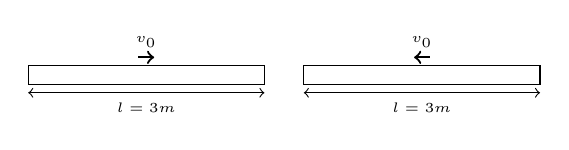
\begin{tikzpicture}
      \draw (0,0) rectangle (3,0.25);
      \draw[<->] (0,-0.1) -- (3,-0.1) node [midway, below] {\tiny $l=3m$};
      \draw[->,thick] (1.4,0.35) -- (1.6,0.35) node [midway, above] {\tiny $v_0$};
      \draw[<->] (3.5,-0.1) -- (6.5,-0.1) node [midway, below] {\tiny $l=3m$};
      \draw[<-,thick] (4.9,0.35) -- (5.1,0.35) node [midway, above] {\tiny $v_0$};
      \draw (3.5,0) rectangle (6.5,0.25);
    \end{tikzpicture}
  \end{block}
  \centering
  \begin{tikzpicture}[scale=0.9]
\begin{axis}[xlabel=$time (s)$,ylabel=$\frac{e}{e_{max}}$,ymajorgrids=true,xmajorgrids=true,legend pos=outer north east]%,title={(c) evolution of total energy $e$}]
\addplot[Red,very thick,mark=none,dashed,mark size=3pt] coordinates {(0.0,0.9876543209876545) (1.2090867953958061e-05,0.997530864197531) (2.4181735907916122e-05,1.0) (3.627260386187418e-05,0.9959104938271608) (4.8363471815832244e-05,0.9894000771604939) (6.045433976979031e-05,0.9840934847608025) (7.254520772374836e-05,0.9813625382788388) (8.463607567770642e-05,0.9805725733439128) (9.672694363166447e-05,0.9803534996362381) (0.00010881781158562253,0.9797373358436207) (0.00012090867953958059,0.97855223305006) (0.00013299954749353864,0.9771562700386213) (0.0001450904154474967,0.9759583476912668) (0.00015718128340145475,0.9751165956200767) (0.0001692721513554128,0.9745300840652308) (0.00018136301930937087,0.9740055540525709) (0.00019345388726332892,0.9734177949795755) (0.00020554475521728698,0.9727609779118863) (0.00021763562317124503,0.9721011582864625) (0.0002297264911252031,0.971500815494294) (0.00024181735907916115,0.9709763284318171) (0.0002539082270331192,0.9705033540228475) (0.0002659990949870773,0.9700475116254563) (0.00027808996294103537,0.9695899456257216) (0.00029018083089499345,0.9691327035661251) (0.00030227169884895153,0.96868819213753) (0.0003143625668029096,0.9682659231600772) (0.0003264534347568677,0.9678664411889574) (0.0003385443027108258,0.9674837019503967) (0.00035063517066478387,0.9671110350826551) (0.00036272603861874195,0.9667453037400304) (0.00037481690657270003,0.9663871533998759) (0.0003869077745266581,0.9660386728300239) (0.0003989986424806162,0.9657010208032414) (0.0004110895104345743,0.9653736208998025) (0.00042318037838853236,0.9650548630015646) (0.00043527124634249045,0.9647432582700906) (0.00044736211429644853,0.9644380781342287) (0.0004594529822504066,0.964139187671229) (0.0004715438502043647,0.9638463458344536) (0.0004836347181583228,0.9635583008484584) (0.0004957255861122808,0.9632716356128425) (0.0005078164540662388,0.9629788582366817) (0.0005199073220201969,0.9626650352466273) (0.0005319981899741549,0.9623025558244344) (0.0005440890579281129,0.9618444966372697) (0.000556179925882071,0.9612184911067746) (0.000568270793836029,0.9603246926454502) (0.000580361661789987,0.959042628998641) (0.000592452529743945,0.9572513419900455) };
\addplot[Duck,thin,mark=*,solid,mark size=2pt] coordinates {(0.0,1.0) (1.2090867953958061e-05,0.9799999999999998) (2.4181735907916122e-05,0.97) (3.627260386187418e-05,0.9624999999999999) (4.8363471815832244e-05,0.9562499999999999) (6.045433976979031e-05,0.9507812499999999) (7.254520772374836e-05,0.9458593750000001) (8.463607567770642e-05,0.94134765625) (9.672694363166447e-05,0.937158203125) (0.00010881781158562253,0.9332305908203123) (0.00012090867953958059,0.9295211791992186) (0.00013299954749353864,0.9259972381591796) (0.0001450904154474967,0.9226334762573243) (0.00015718128340145475,0.9194098711013794) (0.0001692721513554128,0.9163102507591249) (0.00018136301930937087,0.9133213311433792) (0.00019345388726332892,0.9104320421814918) (0.00020554475521728698,0.9076330434996636) (0.00021763562317124503,0.9049163683084772) (0.0002297264911252031,0.902275156317046) (0.00024181735907916115,0.8997034499043367) (0.0002539082270331192,0.8971960361519449) (0.0002659990949870773,0.8947483227269913) (0.00027808996294103537,0.8923562391526049) (0.00029018083089499345,0.8900161573950528) (0.00030227169884895153,0.887724827340783) (0.0003143625668029096,0.8854793238875988) (0.0003264534347568677,0.8832770031931295) (0.0003385443027108258,0.8811154662152247) (0.00035063517066478387,0.8789925281119251) (0.00036272603861874195,0.8769061923897169) (0.00037481690657270003,0.8748546289295456) (0.0003869077745266581,0.8728361552026028) (0.0003989986424806162,0.8708492201276435) (0.0004110895104345743,0.8688923901295775) (0.00042318037838853236,0.8669643370432477) (0.00043527124634249045,0.865063827572437) (0.00044736211429644853,0.8631897140664987) (0.0004594529822504066,0.8613409264187486) (0.0004715438502043647,0.8595164649242585) (0.0004836347181583228,0.8577153939617489) (0.0004957255861122808,0.8559368363862708) (0.0005078164540662388,0.8541799685373229) (0.0005199073220201969,0.8524440157818148) (0.0005319981899741549,0.8507282485234637) (0.0005440890579281129,0.8490319786203213) (0.000556179925882071,0.8473545561605471) (0.000568270793836029,0.8456953665535965) (0.000580361661789987,0.8440538278999112) (0.000592452529743945,0.842429388607202) };
\addplot[Orange,very thick,mark=none,densely dotted,mark size=3pt] coordinates {(0.0,0.9873495834618945) (1.1968737974625153e-05,0.9972230792965134) (2.3937475949250306e-05,1.0) (3.590621392387546e-05,0.996543312249306) (4.787495189850061e-05,0.9916724016989357) (5.9843689873125764e-05,0.9886458260672434) (7.181242784775092e-05,0.9877380525503068) (8.378116582237607e-05,0.9876316182265924) (9.574990379700122e-05,0.9872072095327306) (0.00010771864177162638,0.9862586211196859) (0.00011968737974625153,0.9851624959469047) (0.00013165611772087668,0.9842780087964154) (0.00014362485569550183,0.9836648835656183) (0.000155593593670127,0.9831763602119745) (0.00016756233164475214,0.9826698995825812) (0.0001795310696193773,0.9821135512367487) (0.00019149980759400245,0.9815547588976113) (0.0002034685455686276,0.9810419341151472) (0.00021543728354325275,0.9805830603182993) (0.0002274060215178779,0.9801564013202002) (0.00023937475949250306,0.9797401327914591) (0.0002513434974671282,0.979328388660163) (0.00026331223544175336,0.9789272663692082) (0.0002752809734163785,0.9785432962021172) (0.00028724971139100367,0.9781770579069166) (0.0002992184493656288,0.9778246343106916) (0.000311187187340254,0.9774820931955118) (0.0003231559253148791,0.9771479959874065) (0.0003351246632895043,0.9768228205666122) (0.00034709340126412943,0.9765071704950676) (0.0003590621392387546,0.9762007565377634) (0.00037103087721337974,0.97590260746931) (0.0003829996151880049,0.9756117726801273) (0.00039496835316263004,0.9753277223895899) (0.0004069370911372552,0.9750502574593737) (0.00041890582911188035,0.9747792209216646) (0.0004308745670865055,0.9745143288096212) (0.00044284330506113066,0.9742551920745642) (0.0004548120430357558,0.9740013948706343) (0.00046678078101038096,0.9737524481523462) (0.0004787495189850061,0.9735074554284332) (0.0004907182569596313,0.9732642558608436) (0.0005026869949342565,0.9730175918911446) (0.0005146557329088817,0.972755592971648) (0.0005266244708835069,0.9724538550537384) (0.0005385932088581321,0.9720670387858211) (0.0005505619468327574,0.971519585751107) (0.0005625306848073826,0.9706998361345011) (0.0005744994227820078,0.9694646058920318) (0.000586468160756633,0.9676621151764617) };
\addplot[Blue,very thick,mark=none,solid,mark size=3pt] coordinates {(0.0,0.9999999999999998) (2.4181735907916125e-05,0.9999999999999998) (4.836347181583225e-05,0.9999999999999998) (7.254520772374838e-05,0.9999999999999998) (9.67269436316645e-05,0.9999999999999998) (0.00012090867953958063,0.9999999999999998) (0.00014509041544749675,1.0) (0.0001692721513554129,0.9999999999999998) (0.000193453887263329,0.9999999999999998) (0.00021763562317124512,0.9999999999999998) (0.00024181735907916123,0.9999999999999998) (0.00026599909498707734,0.9999999999999997) (0.00029018083089499345,0.9999999999999997) (0.00031436256680290956,0.9999999999999997) (0.0003385443027108257,0.9999999999999997) (0.0003627260386187418,0.9999999999999997) (0.0003869077745266579,0.9999999999999997) (0.000411089510434574,0.9999999999999997) (0.0004352712463424901,0.9999999999999994) (0.00045945298225040623,0.9999999999999997) (0.00048363471815832235,0.9999999999999994) (0.0005078164540662385,0.9999999999999992) (0.0005319981899741547,0.9999999999999992) (0.0005561799258820708,0.9999999999999992) (0.000580361661789987,0.9999999999999992) (0.0006045433976979032,0.9999999999999992) };
\addplot[Purple,very thick,mark=|,solid,mark size=3pt] coordinates {(0.0,1.0) (1.1968737974625153e-05,0.9849999999999999) (2.3937475949250306e-05,0.9782812499999997) (3.590621392387546e-05,0.9728686523437499) (4.787495189850061e-05,0.9685175323486328) (5.9843689873125764e-05,0.9646764224767683) (7.181242784775092e-05,0.9612245353125033) (8.378116582237607e-05,0.9580584139595156) (9.574990379700122e-05,0.9551170218177228) (0.00010771864177162638,0.9523583400291113) (0.00011968737974625153,0.9497518470633621) (0.00013165611772087668,0.9472747764554426) (0.00014362485569550183,0.9449095127565772) (0.000155593593670127,0.942642119512832) (0.00016756233164475214,0.9404613389338139) (0.0001795310696193773,0.9383579222991295) (0.00019149980759400245,0.9363241607011475) (0.0002034685455686276,0.9343535480062032) (0.00021543728354325275,0.9324405332414724) (0.0002274060215178779,0.9305803349197901) (0.00023937475949250306,0.928768799378865) (0.0002513434974671282,0.9270022910038743) (0.00026331223544175336,0.9252776059761404) (0.0002752809734163785,0.9235919036615065) (0.00028724971139100367,0.9219426514179895) (0.0002992184493656288,0.9203275797465361) (0.000311187187340254,0.9187446455091373) (0.0003231559253148791,0.9171920015078542) (0.0003351246632895043,0.915667971129286) (0.00034709340126412943,0.914171027059833) (0.0003590621392387546,0.9126997733000616) (0.00037103087721337974,0.9112529298736883) (0.0003829996151880049,0.9098293197534216) (0.00039496835316263004,0.9084278576229242) (0.0004069370911372552,0.9070475401691336) (0.00041890582911188035,0.9056874376575983) (0.0004308745670865055,0.9043466865894064) (0.00044284330506113066,0.9030244832746345) (0.0004548120430357558,0.9017200781862146) (0.00046678078101038096,0.9004327709813899) (0.0004787495189850061,0.8991619060967203) (0.0004907182569596313,0.897906868837865) (0.0005026869949342565,0.8966670818978505) (0.0005146557329088817,0.8954420022477787) (0.0005266244708835069,0.8942311183524017) (0.0005385932088581321,0.8930339476700012) (0.0005505619468327574,0.8918500344018717) (0.0005625306848073826,0.8906789474616031) (0.0005744994227820078,0.8895202786384733) (0.000586468160756633,0.8883736409327396) (0.0005984368987312582,0.8872386670435604) };
\addplot[Green,thick,mark=x,only marks,mark size=3pt] coordinates {(0.0,1.0) (2.3937475949250306e-05,0.9999999999999997) (4.787495189850061e-05,0.9999999999999998) (7.181242784775092e-05,0.9999999999999998) (9.574990379700122e-05,0.9999999999999998) (0.00011968737974625153,0.9999999999999998) (0.00014362485569550183,0.9999999999999998) (0.00016756233164475214,0.9999999999999997) (0.00019149980759400245,0.9999999999999997) (0.00021543728354325275,0.9999999999999994) (0.00023937475949250306,0.9999999999999994) (0.00026331223544175336,0.9999999999999992) (0.00028724971139100367,0.999999999999999) (0.000311187187340254,0.999999999999999) (0.0003351246632895043,0.999999999999999) (0.0003590621392387546,0.999999999999999) (0.0003829996151880049,0.999999999999999) (0.0004069370911372552,0.999999999999999) (0.0004308745670865055,0.999999999999999) (0.0004548120430357558,0.999999999999999) (0.0004787495189850061,0.9999999999999989) (0.0005026869949342564,0.999999999999999) (0.0005266244708835067,0.999999999999999) (0.000550561946832757,0.9999999999999989) (0.0005744994227820073,0.9999999999999989) (0.0005984368987312576,0.999999999999999) };
\addplot[black,thin,mark=none,solid,mark size=3pt] coordinates {(0.0,1.0) (1e-08,1.0) };
\legend{usl 1ppc,usl-pic 1ppc,usl 2ppc,dgmpm 1ppc,dgmpm 2ppc,dgmpm 2ppc (RK2),exact}
\end{axis}
\end{tikzpicture}
%%% Local Variables:
%%% mode: latex
%%% TeX-master: "../../mainManuscript"
%%% End:

  \footnoteCite{Wang}
\end{frame}

\begin{frame}{Compression load on a one-dimensional Saint-Venant-Kirchhoff medium \cite{DGMPM}}
  \begin{block}{}
    \centering
    \begin{tikzpicture}[spy using outlines={rectangle, magnification=3, size=2.cm, connect spies},scale=.75]
\begin{groupplot}[group style={group size=2 by 1,
ylabels at=edge left, yticklabels at=edge left,horizontal sep=2.ex,
vertical sep=4ex,xticklabels at=edge bottom,xlabels at=edge bottom},
ymajorgrids=true,xmajorgrids=true,enlargelimits=0,xmin=0.,xmax=6.,xlabel=$x (m)$,
axis on top,scale only axis,width=0.45\linewidth
]
\nextgroupplot[title={(a) $t = 3.92\times 10^{-4} $ s.},ymin=-25000000000,ymax=100,ylabel=$\Pi (Pa)$]
\addplot[Red,solid,mark=square,thick,mark size=2pt,mark repeat=4] coordinates{(0.18113966255624325,-20007387970.557335) (0.23660957067723135,-19988392818.3347) (0.2920788709374843,-20011472871.418236) (0.3475465580979351,-19999236069.727806) (0.40301621336327426,-19998245880.63013) (0.45848806845105955,-19984448351.164803) (0.5139598579950124,-19998686429.534996) (0.5694253122275346,-20027025243.851627) (0.6248879078337095,-20017897149.05008) (0.6803579566733343,-19976931926.095703) (0.7358413922425652,-19927878077.1612) (0.7913241193811056,-19981695225.019558) (0.8467831666341433,-20087015379.390438) (0.9022179154568516,-20144826853.77387) (0.9576641344566965,-20009988053.97157) (1.0131641918337713,-19782733533.209187) (1.0687115307188686,-19691353212.24222) (1.124235928218022,-19937312614.787815) (1.1796571770709081,-20384163154.164658) (1.2349723153124932,-20646777745.580776) (1.2902866680287384,-20389406392.113857) (1.3457489654377526,-19655116047.251022) (1.4014327509400668,-18891326513.439537) (1.4572569378967974,-18697692067.140934) (1.5130091682370217,-19382360949.13436) (1.5684673776430997,-20684465128.886307) (1.6235362200421761,-21967151275.97645) (1.6782985638149688,-22681751921.790474) (1.7329610612897364,-22610456741.048157) (1.7877611264338498,-21794563544.447487) (1.8429024370710971,-20378968726.205227) (1.898532608553216,-18519270034.114338) (1.9547451388785275,-16354096072.585594) (2.011588268801284,-14007489564.652088) (2.0690729759046422,-11597655741.347029) (2.1271787378778857,-9241575329.720287) (2.1858582502503965,-7051805509.823394) (2.2450427346773547,-5125790990.030698) (2.3046488964305416,-3531584621.694986) (2.364587491121773,-2296494660.883612) (2.42477231457793,-1404813762.861708) (2.4851277984388167,-806658783.7726073) (2.5455936523943143,-434313335.0923665) (2.6061260076512562,-219206572.42083678) (2.6666956814435676,-103747943.84912725) (2.7272848711004336,-46072088.863264605) (2.787883582486266,-19209018.54975228) (2.848486633986895,-7523354.327414296) (2.9090915361189578,-2768883.4778968245) (2.969697177276221,-957709.9415031691) (3.0303030950520506,-311276.06559629895) (3.0909091099260717,-95034.93601685615) (3.1515151567697104,-27238.82520180213) (3.2121212134856725,-7323.202979922718) (3.2727272730598322,-1844.8368196336637) (3.3333333334093,-434.89835664335993) (3.3939393939556295,-95.78655390230804) (3.454545454548694,-19.674245139028173) (3.5151515151521173,-3.760269873254174) (3.575757575757679,-0.667039073549019) (3.636363636363653,-0.10948934067082168) (3.6969696969696995,-0.016559403421139835) (3.7575757575757582,-0.0023015777318190745) (3.8181818181818183,-0.0002690155790437879) (3.878787878787879,-2.9890619893754217e-05) (3.9393939393939394,0.0) (4.0,0.0) (4.0606060606060606,0.0) (4.121212121212121,0.0) (4.181818181818182,0.0) (4.242424242424242,0.0) (4.303030303030303,0.0) (4.363636363636363,0.0) (4.424242424242425,0.0) (4.484848484848485,0.0) (4.545454545454546,0.0) (4.606060606060606,0.0) (4.666666666666667,0.0) (4.7272727272727275,0.0) (4.787878787878788,0.0) (4.848484848484849,0.0) (4.909090909090909,0.0) (4.96969696969697,0.0) (5.03030303030303,0.0) (5.090909090909091,0.0) (5.151515151515151,0.0) (5.212121212121212,0.0) (5.2727272727272725,0.0) (5.333333333333334,0.0) (5.3939393939393945,0.0) (5.454545454545455,0.0) (5.515151515151516,0.0) (5.575757575757576,0.0) (5.636363636363637,0.0) (5.696969696969697,0.0) (5.757575757575758,0.0) (5.818181818181818,0.0) (5.878787878787879,0.0) (5.9393939393939394,0.0) (6.0,0.0) };
% \addplot[Green,solid,mark=+,thick,mark size=3pt,mark repeat=8] coordinates{(0.14458016415053374,-4492984179.815072) (0.20700567508876402,-4616851256.085481) (0.26192682032798,-8701783614.471033) (0.3166557679850661,-14769300822.97382) (0.37198979279039157,-10818907987.145092) (0.42389285517095404,-18546143088.853233) (0.4807409661264832,-20038572921.80319) (0.5394075252648387,-18577915141.806976) (0.5928327519832804,-18605471539.882217) (0.6444346551493367,-17206669759.272823) (0.6981089273647494,8898634753.481533) (0.7538338873459312,-3769769274.7046795) (0.8148859022965532,-7877241947.613326) (0.8740167159125545,-10428512098.56688) (0.9322750542449941,-7963151389.194499) (0.9886792326086277,-5415873012.934844) (1.0503792461111,-4899773247.770117) (1.1059023328114148,-6073727795.259949) (1.168182044723453,-8272598895.114129) (1.2239563325491585,-15289412802.07212) (1.2786340981804958,-20553813102.66058) (1.3300218880231578,-23831925765.03392) (1.3864196881847615,-18313045752.99838) (1.4367633619846196,-23473776638.046604) (1.4948452210931042,-13746884954.822872) (1.550374944560456,-4900065712.764751) (1.6105497190516702,-5306150383.525315) (1.667215830784174,9099753256.929346) (1.7279087754072262,536051056.4904309) (1.7846218556951328,-15823096911.347807) (1.840693305028078,-17509762931.97553) (1.8968946493640213,-16795026937.251657) (1.9534982445258748,-15179072528.960943) (2.010642764880971,-13064870753.992636) (2.068373530783145,-10803757181.628149) (2.126679283364548,-8581113823.3979) (2.1855162311522043,-6522979841.143169) (2.2448193109079337,-4723808496.348123) (2.304510336066493,-3244207607.300068) (2.3645062759482824,-2104615987.6256115) (2.424727505193723,-1285737105.3840566) (2.4851046097012044,-738181506.1517382) (2.5455824335843458,-397884299.58068085) (2.606120949719129,-201298837.7471466) (2.6666935643441616,-95624493.38866894) (2.727284052469423,-42679655.45989422) (2.7878832922629995,-17910536.62779694) (2.8484865408425657,-7071474.426653465) (2.9090915096983205,-2628034.233195584) (2.969697171001699,-919579.0254054805) (3.030303094003672,-302975.7832523777) (3.0909091099310815,-93976.35503543683) (3.1515151568720987,-27432.252424758757) (3.212121213542833,-7531.611725312223) (3.272727273082442,-1943.3925302347886) (3.3333333334167734,-470.81612113249076) (3.3939393939578015,-106.96409143033765) (3.4545454545492627,-22.7561175031737) (3.515151515152252,-4.525828429973007) (3.5757575757577094,-0.8398367471548122) (3.6363636363636593,-0.14508906896428295) (3.696969696969701,-0.02325490227734078) (3.7575757575757582,-0.0034374212877817346) (3.8181818181818183,-0.00044835929840631323) (3.878787878787879,-2.9890619893754217e-05) (3.9393939393939394,0.0) (4.0,0.0) (4.0606060606060606,0.0) (4.121212121212121,0.0) (4.181818181818182,0.0) (4.242424242424242,0.0) (4.303030303030303,0.0) (4.363636363636363,0.0) (4.424242424242425,0.0) (4.484848484848485,0.0) (4.545454545454546,0.0) (4.606060606060606,0.0) (4.666666666666667,0.0) (4.7272727272727275,0.0) (4.787878787878788,0.0) (4.848484848484849,0.0) (4.909090909090909,0.0) (4.96969696969697,0.0) (5.03030303030303,0.0) (5.090909090909091,0.0) (5.151515151515151,0.0) (5.212121212121212,0.0) (5.2727272727272725,0.0) (5.333333333333334,0.0) (5.3939393939393945,0.0) (5.454545454545455,0.0) (5.515151515151516,0.0) (5.575757575757576,0.0) (5.636363636363637,0.0) (5.696969696969697,0.0) (5.757575757575758,0.0) (5.818181818181818,0.0) (5.878787878787879,0.0) (5.9393939393939394,0.0) (6.0,0.0) };
\addplot[Blue,solid,mark=asterisk,thick,mark size=3pt,mark repeat=4] coordinates{(0.18223626695430106,-20001038126.338352) (0.23768991437502363,-19998978749.720036) (0.29314649378618063,-20001114659.245598) (0.34860543803553107,-19998938245.2226) (0.4040658491410484,-20001256754.90668) (0.45952782916726886,-19998839045.273113) (0.5149904890937893,-20001474418.40657) (0.5704543859119624,-19998676252.213406) (0.6259184542367701,-20001782405.220955) (0.6813836580819609,-19998441083.411068) (0.7368486397583429,-20002201231.838303) (0.7923147950195939,-19998120374.85034) (0.8477803694219141,-20002758611.22954) (0.9032472602061058,-19997695857.750816) (0.9587131991399028,-20003491433.37429) (1.0141806935506261,-19997143183.71807) (1.0696468176244773,-20004448444.943924) (1.1251148389552674,-19996430638.27334) (1.1805809915705654,-20005693753.570515) (1.236049502978598,-19995517092.631374) (1.2915155327784278,-20007309360.081253) (1.3469845303024321,-19994338279.332916) (1.40245028244176,-20009344487.106834) (1.4579198169262246,-19992551315.62019) (1.513385229630577,-20010820110.039314) (1.56885582799049,-19986004318.92832) (1.6243223609111979,-19998898945.843636) (1.6797993655091994,-19937983836.75768) (1.7352813335683657,-19884506153.093845) (1.7908003238933292,-19661070569.71126) (1.8463726052101397,-19334608195.764057) (1.9020720923142245,-18656825873.30627) (1.9579550525579756,-17730639757.70477) (2.014141675235781,-16293214393.548588) (2.070709720889273,-14546210044.163712) (2.1277940139676583,-12211885498.604748) (2.185461858436101,-9544683527.544516) (2.243846992592119,-6099478616.598052) (2.303030303030303,0.0) (2.3636363636363638,0.0) (2.4242424242424243,0.0) (2.484848484848485,0.0) (2.5454545454545454,0.0) (2.606060606060606,0.0) (2.666666666666667,0.0) (2.7272727272727275,0.0) (2.787878787878788,0.0) (2.8484848484848486,0.0) (2.909090909090909,0.0) (2.9696969696969697,0.0) (3.0303030303030303,0.0) (3.090909090909091,0.0) (3.1515151515151514,0.0) (3.2121212121212124,0.0) (3.272727272727273,0.0) (3.3333333333333335,0.0) (3.393939393939394,0.0) (3.4545454545454546,0.0) (3.515151515151515,0.0) (3.5757575757575757,0.0) (3.6363636363636367,0.0) (3.6969696969696972,0.0) (3.757575757575758,0.0) (3.8181818181818183,0.0) (3.878787878787879,0.0) (3.9393939393939394,0.0) (4.0,0.0) (4.0606060606060606,0.0) (4.121212121212121,0.0) (4.181818181818182,0.0) (4.242424242424242,0.0) (4.303030303030303,0.0) (4.363636363636363,0.0) (4.424242424242425,0.0) (4.484848484848485,0.0) (4.545454545454546,0.0) (4.606060606060606,0.0) (4.666666666666667,0.0) (4.7272727272727275,0.0) (4.787878787878788,0.0) (4.848484848484849,0.0) (4.909090909090909,0.0) (4.96969696969697,0.0) (5.03030303030303,0.0) (5.090909090909091,0.0) (5.151515151515151,0.0) (5.212121212121212,0.0) (5.2727272727272725,0.0) (5.333333333333334,0.0) (5.3939393939393945,0.0) (5.454545454545455,0.0) (5.515151515151516,0.0) (5.575757575757576,0.0) (5.636363636363637,0.0) (5.696969696969697,0.0) (5.757575757575758,0.0) (5.818181818181818,0.0) (5.878787878787879,0.0) (5.9393939393939394,0.0) (6.0,0.0) };
\addplot[Orange,solid,mark=*,thick,mark size=2pt,mark repeat=8] coordinates{(0.18040294251455286,-19999905863.699165) (0.20808627061289414,-19999751264.69732) (0.23556978374946896,-19999562658.846558) (0.26327345885715725,-19999407507.436043) (0.29075488519191395,-19999217896.661182) (0.31846367610917153,-19999061632.237038) (0.34594307399070734,-19998870329.12512) (0.37365434446212986,-19998712373.70647) (0.40113240076996964,-19998518664.39632) (0.42884521261398156,-19998358413.125576) (0.4563223312033673,-19998161545.344017) (0.4840362256600238,-19997998355.95089) (0.5115126530249403,-19997797525.55417) (0.5392273662627345,-19997630706.324066) (0.5667032640683534,-19997425041.735966) (0.594418628493124,-19997253837.40594) (0.6218941093312814,-19997042381.17444) (0.6496100110819408,-19996865956.008568) (0.6770851572446662,-19996647642.458878) (0.704801515178081,-19996465059.50123) (0.7322763892505872,-19996238687.100967) (0.7599931434930574,-19996048882.231777) (0.7874677947186973,-19995813078.746506) (0.81518489996572,-19995614827.601215) (0.8426593682826082,-19995368005.289177) (0.8703767896598259,-19995159880.177517) (0.8978511083867168,-19994900176.812107) (0.92556881878857,-19994680488.79575) (0.953043016495599,-19994405686.410156) (0.9807609948285569,-19994172400.296314) (1.008235096706118,-19993879795.801735) (1.0359533267236931,-19993630366.8231) (1.0634273556585923,-19993316472.931572) (1.0911458252461372,-19993047351.183105) (1.118619802833324,-19992706835.253857) (1.146338503851824,-19992411476.050125) (1.1738124519262572,-19992032791.59899) (1.2015313814999844,-19991693634.279457) (1.2290053262789837,-19991242130.638687) (1.25672449299276,-19990801780.147366) (1.2841984788394833,-19990162680.559273) (1.3119179247098083,-19989434921.047157) (1.3393920576107705,-19988249014.161484) (1.3671119240169711,-19986685992.314224) (1.3945864926570357,-19983950456.46633) (1.422307190002744,-19980133159.696182) (1.4497829566734648,-19973396502.77201) (1.4775055374660702,-19964121363.32016) (1.5049843341052282,-19948173674.81723) (1.532711187365164,-19927167256.47763) (1.5601969418987578,-19892428871.300217) (1.5879328684153249,-19849076630.679882) (1.6154330527396683,-19780384053.949062) (1.643186604598769,-19699233952.465065) (1.6707138204447796,-19576060639.37215) (1.6984985402324504,-19437863578.19648) (1.7260716661806943,-19236691492.035503) (1.75390670241847,-19021116192.28342) (1.781550955385115,-18719618500.228672) (1.8094606309171823,-18408860684.58476) (1.837206202568401,-17990477870.76324) (1.865218468892651,-17572517252.88768) (1.893097944642736,-17029814086.17729) (1.9212420512305401,-16500433110.299011) (1.9492872554636622,-15836433782.008884) (1.9775911554035532,-15199911582.726149) (2.005830141198215,-14427681448.259727) (2.0343180795772975,-13696656439.56188) (2.062772737790181,-12837968682.129587) (2.0914632521857817,-12033022242.120184) (2.1201476816132794,-11116848246.643755) (2.14905205398078,-10266019602.50983) (2.1779716087449765,-9327094310.705921) (2.207092741841568,-8465044635.551027) (2.2362436214513863,-7542212976.516653) (2.2655753786348134,-6708336979.026626) (2.2949447174689688,-5842014349.592722) (2.324471907719638,-5076703860.063381) (2.354038474552135,-4304807308.930284) (2.383737780790947,-3643631733.309597) (2.413473506765107,-2996015694.5501895) (2.443315603702364,-2462925787.067946) (2.473188090048969,-1955670864.4132829) (2.503140874115482,-1557827332.4962366) (2.5331167115351088,-1189903472.3026366) (2.5631490487515123,-916956502.8075399) (2.5931973176751666,-671475286.956899) (2.6232823284753723,-500156639.3655174) (2.6533773696952254,-350189648.52024174) (2.683494363096932,-252076641.13416293) (2.713617108123326,-168404463.10215867) (2.743751862249033,-117182561.85249747) (2.7738896206741313,-74583282.90579824) (2.8040333857626796,-50198256.60739492) (2.834178581287497,-30402448.092186444) (2.8643265233525126,-19806900.387403697) (2.8944750868610085,-11403539.039500952) (2.9246247990660907,-7197050.42870293) (2.9547747578826424,-3935184.952863811) (2.984925156472305,-2407871.3282750887) (3.0150756445417084,-1249111.1449670813) (3.0452262868427633,-741581.2353492869) (3.07537695885081,-364599.5168943291) (3.1055276804354097,-210177.375886844) (3.135678411048561,-97816.78080674187) (3.1658291562722796,-54790.33514606749) (3.1959799040083476,-24105.68801215534) (3.2261306556922738,-13128.815579857537) (3.256281408016224,-5452.248657437644) (3.2864321613179936,-2889.207724514482) (3.3165829147689725,-1130.6496674298353) (3.346733668441846,-583.3075249485646) (3.376884422146529,-214.692784746355) (3.4070351758973105,-107.89733632141935) (3.4371859296542877,-37.270374815403535) (3.467336683420022,-18.256831942428335) (3.4974874371868587,-5.903905569425186) (3.527638190955214,-2.8202995494257412) (3.5577889447237485,-0.851374526431109) (3.5879396984925225,-0.39673819784921505) (3.6180904522613226,-0.11128277786440094) (3.6482412060301583,-0.050485257000541406) (3.6783919597989967,-0.012912747794101202) (3.7085427135678395,-0.005649327159919428) (3.738693467336683,-0.0011358435559626553) (3.7688442211055273,-0.00044835929840631247) (3.798994974874372,-5.9781239787508415e-05) (3.829145728643216,0.0) (3.85929648241206,0.0) (3.8894472361809043,0.0) (3.9195979899497484,0.0) (3.949748743718593,0.0) (3.979899497487437,0.0) (4.010050251256281,0.0) (4.040201005025126,0.0) (4.0703517587939695,-5.9781239787508415e-05) (4.100502512562814,5.978123978750844e-05) (4.130653266331658,-5.9781239787508415e-05) (4.160804020100502,0.0) (4.190954773869347,0.0) (4.221105527638191,0.0) (4.251256281407035,0.0) (4.281407035175879,0.0) (4.311557788944723,0.0) (4.341708542713568,0.0) (4.371859296482412,-5.9781239787508415e-05) (4.402010050251256,5.978123978750844e-05) (4.4321608040201,-5.9781239787508415e-05) (4.4623115577889445,0.0) (4.492462311557789,0.0) (4.522613065326633,0.0) (4.552763819095477,0.0) (4.582914572864321,0.0) (4.613065326633166,0.0) (4.64321608040201,0.0) (4.673366834170854,-5.9781239787508415e-05) (4.703517587939698,0.0) (4.733668341708542,-5.9781239787508415e-05) (4.763819095477387,0.0) (4.793969849246231,0.0) (4.824120603015075,0.0) (4.8542713567839195,0.0) (4.884422110552763,0.0) (4.914572864321608,0.0) (4.944723618090452,0.0) (4.974874371859296,-5.9781239787508415e-05) (5.005025125628141,0.0) (5.035175879396984,-5.9781239787508415e-05) (5.065326633165829,0.0) (5.0954773869346734,0.0) (5.125628140703517,0.0) (5.155778894472362,0.0) (5.185929648241205,0.0) (5.21608040201005,0.0) (5.2462311557788945,0.0) (5.276381909547738,0.0) (5.306532663316583,0.0) (5.3366834170854265,-5.9781239787508415e-05) (5.366834170854271,0.0) (5.396984924623116,0.0) (5.427135678391959,0.0) (5.457286432160804,0.0) (5.487437185929648,0.0) (5.517587939698492,0.0) (5.547738693467337,0.0) (5.57788944723618,-5.9781239787508415e-05) (5.608040201005025,5.978123978750844e-05) (5.638190954773869,-5.9781239787508415e-05) (5.668341708542713,0.0) (5.698492462311558,0.0) (5.7286432160804015,0.0) (5.758793969849246,0.0) (5.788944723618091,0.0) (5.819095477386934,-5.9781239787508415e-05) (5.849246231155779,5.978123978750844e-05) (5.879396984924623,-5.9781239787508415e-05) (5.909547738693467,0.0) (5.939698492462312,0.0) (5.969849246231155,0.0) (6.0,0.0) };
\addplot[Purple,solid,mark=x,thick,mark size=3pt,mark repeat=8] coordinates{(0.18131378718277094,-19999262093.34344) (0.2111551896038996,-19999208437.799057) (0.23643541487598752,-20000224760.504063) (0.26641626606217844,-20000228491.7252) (0.2916325167231138,-19998707378.854794) (0.32161966011673226,-19998594611.356926) (0.34683927867015524,-19999694040.17497) (0.37681266646788564,-19999757554.504402) (0.4020454222245936,-19998097246.860916) (0.43200405056315605,-19997919365.19895) (0.45724952198519836,-19999191246.821526) (0.4871948903809219,-19999321280.513092) (0.5124520623782097,-19997417635.65041) (0.5423860171791831,-19997163934.154667) (0.5676529969062377,-19998710584.515995) (0.5975768390098147,-19998918735.01063) (0.6228530757957436,-19996649627.093723) (0.6527681513527388,-19996303887.6553) (0.6780519389382945,-19998248302.73336) (0.7079590524289994,-19998551913.140324) (0.7332504459993936,-19995768070.802536) (0.7631506154960541,-19995307328.901688) (0.7884479122147041,-19997802451.917274) (0.8183416111799895,-19998225927.376953) (0.8436454063337837,-19994739605.6622) (0.8735334785602806,-19994132386.35754) (0.8988418965443941,-19997372626.61143) (0.9287245729443043,-19997949278.379314) (0.9540387589882052,-19993519843.306847) (0.9839168058344933,-19992723721.05861) (1.0092345514370695,-19996959588.419666) (1.0391079965615078,-19997734141.172607) (1.0644310684103957,-19992049400.191372) (1.0943006706635163,-19991007680.65578) (1.119626356134282,-19996564675.33873) (1.149491950282052,-19997596620.74697) (1.1748227655265604,-19990248485.38932) (1.2046851629266173,-19988885733.251534) (1.2300176883339518,-19996189208.64802) (1.2598765194647277,-19997557210.98869) (1.2852142100722175,-19988010284.97481) (1.315070398193668,-19986226124.41762) (1.340408873760237,-19995834462.491627) (1.3702618151847368,-19997640618.95407) (1.3956057331986196,-19985185794.717686) (1.425456529142571,-19982838399.544888) (1.4508002262192339,-19995441210.93962) (1.4806479919474025,-19997774383.794014) (1.5059977047971904,-19981210528.03947) (1.535843810124145,-19977918753.02119) (1.5611922676411227,-19993205119.19054) (1.5910355305315467,-19995452591.198547) (1.616391432027266,-19968598456.42914) (1.6462337798635807,-19961594343.18897) (1.6715890745594983,-19964843222.356018) (1.7014295017064016,-19960253912.475136) (1.726799922936672,-19878285913.100418) (1.756642363788195,-19851557351.793938) (1.7820274962342342,-19747992863.74265) (1.8118735068310567,-19707656010.39773) (1.8373138716415776,-19391671979.45249) (1.8671728213446566,-19302467480.826202) (1.8926983478367085,-18831862219.67902) (1.9225769044007963,-18708844166.234917) (1.9482762302248442,-17842734916.52506) (1.9781885168185271,-17655637693.430443) (2.004129221682268,-16520369545.901424) (2.0340814998294934,-16308015641.958086) (2.060387863504825,-14659571679.163057) (2.090390173092113,-14395669380.348734) (2.1171380016887316,-12441160095.683947) (2.1471859718500714,-12198478167.923162) (2.1745057715007627,-9642398941.211975) (2.204601458900404,-9347973351.850803) (2.23256759612502,-6295444226.197402) (2.2626858991584435,-6155926493.817503) (2.2914572864321605,0.0006575936376625943) (2.321608040201005,0.0006575936376625943) (2.351758793969849,0.0006575936376625943) (2.3819095477386933,0.0005978123978750856) (2.4120603015075375,0.00023912495915003393) (2.4422110552763816,0.0001793437193625254) (2.472361809045226,0.0005978123978750856) (2.5025125628140703,0.0005978123978750856) (2.5326633165829144,0.0003586874387250511) (2.5628140703517586,0.0003586874387250511) (2.5929648241206027,0.0007771561172376117) (2.6231155778894473,0.000717374877450103) (2.6532663316582914,0.0005978123978750856) (2.6834170854271355,0.0005978123978750856) (2.7135678391959797,0.0005380311580875769) (2.743718592964824,0.0005380311580875769) (2.7738693467336684,0.0004782499183000683) (2.8040201005025125,0.0004782499183000683) (2.8341708542713566,0.0004782499183000683) (2.8643216080402008,0.0004782499183000683) (2.8944723618090453,0.0005380311580875769) (2.9246231155778895,0.0005380311580875769) (2.9547738693467336,0.0005380311580875769) (2.9849246231155777,0.0005380311580875769) (3.015075376884422,0.0002989061989375425) (3.0452261306532664,0.00023912495915003393) (3.0753768844221105,0.0005380311580875769) (3.1055276381909547,0.0005380311580875769) (3.135678391959799,0.0003586874387250511) (3.165829145728643,0.0002989061989375425) (3.1959798994974875,0.0006575936376625943) (3.2261306532663316,0.0005978123978750856) (3.2562814070351758,5.978123978750844e-05) (3.28643216080402,0.0) (3.316582914572864,0.0005978123978750856) (3.3467336683417086,0.0005978123978750856) (3.3768844221105527,0.0003586874387250511) (3.407035175879397,0.0003586874387250511) (3.437185929648241,-0.0001195624795750168) (3.467336683417085,-0.0001195624795750168) (3.4974874371859297,0.0004782499183000683) (3.527638190954774,0.0004782499183000683) (3.557788944723618,0.0001793437193625254) (3.587939698492462,0.0001793437193625254) (3.618090452261306,0.0005978123978750856) (3.648241206030151,0.0004782499183000683) (3.678391959798995,5.978123978750844e-05) (3.708542713567839,0.0) (3.738693467336683,-0.0001195624795750168) (3.7688442211055273,-0.0001195624795750168) (3.798994974874372,0.0005380311580875769) (3.829145728643216,0.0005380311580875769) (3.85929648241206,0.00023912495915003393) (3.8894472361809043,0.0001793437193625254) (3.9195979899497484,-0.0002391249591500335) (3.949748743718593,-0.0002391249591500335) (3.979899497487437,0.0006575936376625943) (4.010050251256281,0.0005978123978750856) (4.040201005025126,5.978123978750844e-05) (4.0703517587939695,0.0) (4.100502512562814,0.0002989061989375425) (4.130653266331658,0.0002989061989375425) (4.160804020100502,0.0002989061989375425) (4.190954773869347,0.0002989061989375425) (4.221105527638191,-0.00017934371936252516) (4.251256281407035,-0.0002391249591500335) (4.281407035175879,0.000717374877450103) (4.311557788944723,0.0006575936376625943) (4.341708542713568,-0.0001195624795750168) (4.371859296482412,-0.00017934371936252516) (4.402010050251256,0.0002989061989375425) (4.4321608040201,0.0002989061989375425) (4.4623115577889445,0.00011956247957501691) (4.492462311557789,0.00011956247957501691) (4.522613065326633,0.0004782499183000683) (4.552763819095477,0.0004782499183000683) (4.582914572864321,0.0004782499183000683) (4.613065326633166,0.0004184686785125597) (4.64321608040201,-0.0001195624795750168) (4.673366834170854,-0.0001195624795750168) (4.703517587939698,0.0005978123978750856) (4.733668341708542,0.0005978123978750856) (4.763819095477387,-0.0002391249591500335) (4.793969849246231,-0.00017934371936252516) (4.824120603015075,0.0006575936376625943) (4.8542713567839195,0.0005978123978750856) (4.884422110552763,-0.00032879681883129597) (4.914572864321608,-0.0003885780586188042) (4.944723618090452,0.0004184686785125597) (4.974874371859296,0.0004184686785125597) (5.005025125628141,0.00023912495915003393) (5.035175879396984,0.0001793437193625254) (5.065326633165829,-0.00044835929840631247) (5.0954773869346734,-0.00044835929840631247) (5.125628140703517,0.0005380311580875769) (5.155778894472362,0.0004782499183000683) (5.185929648241205,0.0001793437193625254) (5.21608040201005,0.00011956247957501691) (5.2462311557788945,-0.0002391249591500335) (5.276381909547738,-0.0002391249591500335) (5.306532663316583,0.0004782499183000683) (5.3366834170854265,0.0004782499183000683) (5.366834170854271,-0.00044835929840631247) (5.396984924623116,-0.0005081405381938207) (5.427135678391959,0.0005978123978750856) (5.457286432160804,0.0005978123978750856) (5.487437185929648,-0.0003885780586188042) (5.517587939698492,-0.00044835929840631247) (5.547738693467337,0.000717374877450103) (5.57788944723618,0.0006575936376625943) (5.608040201005025,-0.0001195624795750168) (5.638190954773869,-0.0001195624795750168) (5.668341708542713,-0.00032879681883129597) (5.698492462311558,-0.00032879681883129597) (5.7286432160804015,0.0005380311580875769) (5.758793969849246,0.0004782499183000683) (5.788944723618091,-0.0002391249591500335) (5.819095477386934,-0.00029890619893754183) (5.849246231155779,0.0005978123978750856) (5.879396984924623,0.0005978123978750856) (5.909547738693467,-0.0003885780586188042) (5.939698492462312,-0.0002391249591500335) (5.969849246231155,0.0006575936376625943) (6.0,0.0003586874387250511) };
\addplot[black,solid,mark=none,thick,mark size=2pt,mark repeat=8] coordinates{(0.18223626695430106,-19999999999.99513) (0.23768991437502363,-19999999999.99513) (0.29314649378618063,-19999999999.99513) (0.34860543803553107,-19999999999.99513) (0.4040658491410484,-19999999999.99513) (0.45952782916726886,-19999999999.99513) (0.5149904890937893,-19999999999.99513) (0.5704543859119624,-19999999999.99513) (0.6259184542367701,-19999999999.99513) (0.6813836580819609,-19999999999.99513) (0.7368486397583429,-19999999999.99513) (0.7923147950195939,-19999999999.99513) (0.8477803694219141,-19999999999.99513) (0.9032472602061058,-19999999999.99513) (0.9587131991399028,-19999999999.99513) (1.0141806935506261,-19999999999.99513) (1.0696468176244773,-19999999999.99513) (1.1251148389552674,-19999999999.99513) (1.1805809915705654,-19999999999.99513) (1.236049502978598,-19999999999.99513) (1.2915155327784278,-19999999999.99513) (1.3469845303024321,-19999999999.99513) (1.40245028244176,-19999999999.99513) (1.4579198169262246,-19999999999.99513) (1.513385229630577,-19999999999.99513) (1.56885582799049,-19999999999.99513) (1.6243223609111979,-19999999999.99513) (1.6797993655091994,-19999999999.99513) (1.7352813335683657,-19999999999.99513) (1.7908003238933292,-19999999999.99513) (1.8463726052101397,-19999999999.99513) (1.9020720923142245,-19999999999.99513) (1.9579550525579756,-19999999999.99513) (2.014141675235781,-19999999999.99513) (2.070709720889273,-16666611023.003479) (2.1277940139676583,-12904289824.44056) (2.185461858436101,-8878289746.458426) (2.243846992592119,-4579787187.179763) (2.303030303030303,-5.9781239787508415e-05) (2.3636363636363638,0.0) (2.4242424242424243,0.0) (2.484848484848485,0.0) (2.5454545454545454,0.0) (2.606060606060606,0.0) (2.666666666666667,0.0) (2.7272727272727275,0.0) (2.787878787878788,0.0) (2.8484848484848486,0.0) (2.909090909090909,0.0) (2.9696969696969697,0.0) (3.0303030303030303,0.0) (3.090909090909091,0.0) (3.1515151515151514,0.0) (3.2121212121212124,0.0) (3.272727272727273,0.0) (3.3333333333333335,0.0) (3.393939393939394,0.0) (3.4545454545454546,0.0) (3.515151515151515,0.0) (3.5757575757575757,0.0) (3.6363636363636367,0.0) (3.6969696969696972,0.0) (3.757575757575758,0.0) (3.8181818181818183,0.0) (3.878787878787879,0.0) (3.9393939393939394,0.0) (4.0,0.0) (4.0606060606060606,0.0) (4.121212121212121,0.0) (4.181818181818182,0.0) (4.242424242424242,0.0) (4.303030303030303,0.0) (4.363636363636363,0.0) (4.424242424242425,0.0) (4.484848484848485,0.0) (4.545454545454546,0.0) (4.606060606060606,0.0) (4.666666666666667,0.0) (4.7272727272727275,0.0) (4.787878787878788,0.0) (4.848484848484849,0.0) (4.909090909090909,0.0) (4.96969696969697,0.0) (5.03030303030303,0.0) (5.090909090909091,0.0) (5.151515151515151,0.0) (5.212121212121212,0.0) (5.2727272727272725,0.0) (5.333333333333334,0.0) (5.3939393939393945,0.0) (5.454545454545455,0.0) (5.515151515151516,0.0) (5.575757575757576,0.0) (5.636363636363637,0.0) (5.696969696969697,0.0) (5.757575757575758,0.0) (5.818181818181818,0.0) (5.878787878787879,0.0) (5.9393939393939394,0.0) (6.0,0.0) };
\nextgroupplot[title={(b) $t = 8.67\times 10^{-4} $ s.},ymin=-25000000000,ymax=100,legend style={at={($(0.5,-0.35)+(8.6cm,8cm)$)},legend columns=1}]
\addplot[Red,solid,mark=square,thick,mark size=2pt,mark repeat=4] coordinates{(0.40215869672008975,-20002966107.69059) (0.457627966785195,-19997104751.50747) (0.513097286800686,-20002630395.116173) (0.5685665384345838,-19997564383.50892) (0.6240358914059912,-20001949307.59647) (0.6795051354215621,-19998296730.555145) (0.7349745104449505,-20001068794.2215) (0.7904437566639009,-19999162477.735077) (0.8459131392867446,-20000151998.735622) (0.9013824041972991,-19999953658.369846) (0.9568517903327788,-19999337211.295033) (1.0123210791161483,-20000607983.532116) (1.0677904472000752,-19998804203.13356) (1.123259760747113,-20000974534.75027) (1.1787291362420609,-19998387824.963604) (1.2341985014366061,-20001043765.144054) (1.2896678589785575,-19998439261.46053) (1.3451371978729505,-20001169097.69894) (1.4006065327090447,-19998466539.056812) (1.4560759672115082,-20000499224.49699) (1.5115454187715343,-19998351887.564476) (1.5670148379250948,-20000717034.295868) (1.6224840737690875,-19999583980.693554) (1.6779533341339892,-20000552224.87672) (1.7334228115200356,-19998125296.286465) (1.7888926157575349,-19998355351.277897) (1.8443622894706484,-19999002606.519222) (1.8998313873898136,-20002225389.655373) (1.9552999825026012,-20002382055.115257) (2.0107690526556494,-19999032558.345886) (2.06623944646083,-19993485122.951336) (2.1217106924074174,-19993304706.951477) (2.177180799783086,-20001138115.954144) (2.2326481983780964,-20011510333.319443) (2.28811401488845,-20011770488.502438) (2.3435820983684774,-19996274507.270008) (2.399055550896097,-19975679712.898182) (2.4545325709243824,-19972289707.75089) (2.510006185697169,-19998572556.059826) (2.5654698638893327,-20039069237.649754) (2.6209250127903627,-20055872282.196777) (2.6763829416629408,-20020394239.487396) (2.7318572058777826,-19946080225.620945) (2.787350822291033,-19890219678.193184) (2.8428492036308146,-19914014031.24824) (2.8983273056284653,-20026623198.624027) (2.9537686541200046,-20160878329.021133) (3.009182643474434,-20210122553.559795) (3.064604898729306,-20105453051.971497) (3.1200766121488175,-19877963863.226173) (3.175614527543546,-19659564852.673016) (3.231191847061467,-19611917470.63196) (3.2867457601131416,-19817617224.401936) (3.34221135878627,-20206453601.772022) (3.3975631395954315,-20579887367.368347) (3.4528377580111456,-20720779585.719208) (3.5081230039644167,-20509152468.805176) (3.563518839497915,-19982159129.048527) (3.6190899098052736,-19329723009.997402) (3.674830228910923,-18832678426.2488) (3.730655768192034,-18747186411.447487) (3.786431601244316,-19172666621.4785) (3.842024567371256,-19989991470.92411) (3.8973557343436807,-20930473484.867847) (3.952425118062564,-21722318352.42074) (4.007300555952745,-22197262458.885387) (4.0620860090613045,-22305136668.171135) (4.116890794619843,-22072335300.69355) (4.171811090985546,-21555815239.712955) (4.2269234721701165,-20814879757.268692) (4.282285529759303,-19899709169.050827) (4.337939197218452,-18849305360.96853) (4.393914355989471,-17693238879.57013) (4.4502317836292775,-16454352909.284187) (4.50690525157342,-15151334991.473465) (4.563942860812882,-13800875423.510624) (4.621347771449163,-12419408014.09022) (4.679118478861856,-11024463548.075926) (4.737248777544566,-9635606673.659077) (4.795727554326026,-8274847214.570022) (4.854538565791211,-6966366976.951551) (4.913660368746935,-5735427279.987068) (4.973066569538447,-4606452319.436187) (5.032726519851033,-3600513313.2194457) (5.092606504440273,-2732701320.925401) (5.152671349525113,-2010050131.8525975) (5.2128862600891575,-1430630336.3802323) (5.273218613027733,-984140156.4626706) (5.333639426318369,-653864097.6073364) (5.394124299625824,-419456538.6177206) (5.454653751640019,-259819905.48975244) (5.515213014920877,-155444422.10904887) (5.575791444399964,-89867647.74810077) (5.636381729245206,-50234816.779882476) (5.69697907607438,-27165560.050610524) (5.757580478521224,-14215154.365463901) (5.81818412988482,-7188624.389460928) (5.878788989411862,-3482145.2511414075) (5.939394484991903,-1537812.892742608) (6.000000324003731,-430952.4139511057) };
% \addplot[Green,solid,mark=+,thick,mark size=3pt,mark repeat=8] coordinates{(0.3305960246293847,-1195815550.1995971) (0.39161230760334026,-3001751486.4163485) (0.4454413102167849,-5637412103.086817) (0.502246017766575,-8211738065.932363) (0.554889371361832,-3648179187.2973967) (0.6040556488414989,-10163946106.486933) (0.6607756767836903,-15414976468.499628) (0.7110849211772252,-18402806321.96861) (0.7641049713416583,4372838619.50665) (0.8103197645207294,-15957444288.162867) (0.8681174161223143,-6535126027.305331) (0.9145191755597188,-17299223723.954403) (0.9760168516487829,-9103756949.732803) (1.0363500006243735,-6944949877.393358) (1.0911546496902844,-3780484361.7150283) (1.143987033377203,940863940.0532544) (1.211280372145826,-2136702750.3468308) (1.2600328349670065,-16791957633.697573) (1.318298161079003,-19882797696.837044) (1.3734483670753377,-3783917412.2027526) (1.4230740931526513,-16941799460.448025) (1.4776230224392126,-9195626118.034966) (1.5361530182041787,-13451469966.821522) (1.5894771848609988,-17782103155.37679) (1.6455493653194202,-13872482945.030848) (1.7032470228763343,-10133273406.186687) (1.7557451095988184,-5093208096.238998) (1.8123013009845157,1505441360.3029547) (1.8740127069387826,2514842296.760774) (1.9276438639346298,-7494186663.638683) (1.9863257249046402,-15165756260.53947) (2.0386705692897342,-14610013473.880955) (2.092951294894796,4200874535.183841) (2.152146922484314,2475720046.5561366) (2.206490772333045,-9578261567.709154) (2.2636271290354877,-14527213419.664602) (2.321526729345961,-14047763387.067022) (2.377497106584818,-16117572645.872097) (2.434613274757651,-14024719232.529373) (2.4917665079268043,-11242483571.53254) (2.5475874697334984,-6475662270.246997) (2.604448973972306,-1682622232.240747) (2.6662238948187365,-436618549.11559886) (2.7249170302002748,-4777609640.235831) (2.7820750193855837,-12868390639.490246) (2.839477106093687,-18832264543.465874) (2.8941082104265514,-20596620217.49518) (2.948289064776381,-18556794270.730465) (3.0015727067748457,-7367355706.930192) (3.0618531590394533,39419859.280396774) (3.118697629451758,-6529661866.476899) (3.1792122726226055,-6368695036.875538) (3.235781636646519,-11950350655.473137) (3.2948751175720257,-12847149772.924097) (3.351008178198855,-11160254030.563177) (3.411541431512924,-6883703064.008913) (3.4693534134709534,-2677672008.5077314) (3.5310042809504543,-2086482153.3409517) (3.5876625209014708,-5871221885.214903) (3.6487217630334525,-9879722461.594193) (3.7029689555391214,-18506396979.07718) (3.759858619107299,-18385770255.393757) (3.812132641937167,-21832779395.616787) (3.869632320845837,-20708402549.67381) (3.9219607003872796,-14133712486.782549) (3.9814663662742613,-12440223642.24161) (4.035935544006736,-10481617126.436337) (4.096030524928356,-2624186152.2915626) (4.152857751001601,-5295087841.643626) (4.214313582491814,3567008153.912993) (4.272374370224572,-10804600137.252241) (4.332480556544939,-1982446941.6830957) (4.390641084895692,-10343100968.020914) (4.4480070813791714,-13172896106.347918) (4.505271980058936,-13311192907.308647) (4.562696703758493,-12578769210.610905) (4.620383947645366,-11510752270.526447) (4.6783741561585295,-10306356565.625633) (4.736680153158918,-9053467479.059502) (4.795300547004881,-7800800290.304055) (4.854224943921561,-6583612541.946681) (4.913436105565393,-5431811548.097768) (4.972911149218158,-4371611911.29186) (5.032622641751589,-3424594913.865768) (5.0925399211965665,-2605908542.3101654) (5.152630702969546,-1922698060.4276078) (5.21286284861717,-1373503134.8876824) (5.273206071749562,-948957621.380283) (5.333633336979227,-633676868.8939521) (5.394121769611855,-408848125.3562511) (5.454653007838895,-254882795.87448072) (5.515213050207994,-153577085.0720251) (5.575791738041566,-89478909.41246594) (5.636382045029125,-50438976.74875333) (5.69697932901904,-27523167.224921327) (5.757580654579378,-14541565.002762917) (5.81818424224597,-7428358.017326818) (5.878789057594589,-3634970.1542755133) (5.939394526743113,-1619833.7695637867) (6.000000353648376,-456498.0246249192) };
\addplot[Blue,solid,mark=asterisk,thick,mark size=3pt,mark repeat=4] coordinates{(0.40323447351788533,-19999992851.39263) (0.4586881010429231,-19999975550.817196) (0.5141447567695451,-19999961319.822983) (0.5696036400410711,-19999943949.590042) (0.6250642081503178,-19999929921.24512) (0.6805260821576966,-19999912405.738873) (0.7359889888005496,-19999898728.702877) (0.7914527276883071,-19999880979.932472) (0.8469171467016672,-19999867824.14433) (0.9023821304998236,-19999849734.385986) (0.9578475872619788,-19999837301.51726) (1.0133134462017366,-19999818734.455585) (1.068779648028316,-19999807270.46856) (1.124246147265943,-19999788050.172337) (1.1797129032995322,-19999777860.827866) (1.2351798860997367,-19999757757.735844) (1.290647066240205,-19999749228.106987) (1.3461144237729694,-19999727940.98239) (1.4015819361000685,-19999721560.311665) (1.457049590322891,-19999698692.831535) (1.5125173679340431,-19999695086.44996) (1.567985261358444,-19999670116.707153) (1.6234532543108777,-19999670087.236347) (1.6789213436076955,-19999642327.918293) (1.7343895137791763,-19999646908.643208) (1.7898577656321448,-19999615454.97939) (1.845326083326302,-19999625979.155453) (1.9007944716578893,-19999589640.843777) (1.9562629132913503,-19999607831.85647) (2.011731417355856,-19999565044.031548) (2.067199963836595,-19999593132.843384) (2.1226685668778478,-19999541839.648006) (2.1781372024355146,-19999582717.970844) (2.2336058907216207,-19999520220.34686) (2.2890746020380326,-19999577640.614082) (2.3445433641534326,-19999500397.396103) (2.4000121396933554,-19999579234.0926) (2.455480966009636,-19999482602.214256) (2.5109497954833415,-19999589193.73842) (2.5664186777559044,-19999467089.12925) (2.621887551664038,-19999609685.47611) (2.6773564827178307,-19999454140.782448) (2.732825391940225,-19999643490.480183) (2.7882943654178596,-19999444078.758595) (2.843763300813485,-19999694199.337215) (2.899232310965111,-19999437283.933777) (2.9547012629518656,-19999766474.675694) (3.0101703044489394,-19999434234.0541) (3.065639262529455,-19999866408.947777) (3.1211083302847125,-19999435570.129745) (3.176577282478291,-20000002012.779297) (3.232046371452465,-19999442201.152195) (3.2875153035860043,-20000183850.379253) (3.342984408570345,-19999455339.49994) (3.3984533034186075,-20000425406.55578) (3.453922418963418,-19999474836.55652) (3.509391255847456,-20000737870.25393) (3.564860378533561,-19999479349.572056) (3.6203291400637463,-20001072157.643166) (3.6757982924371264,-19999261975.94895) (3.7312670299231128,-20000894671.113735) (3.7867364343529872,-19997404353.59923) (3.8422056868452303,-19996901850.131256) (3.8976767127703367,-19986589447.349785) (3.953149476046555,-19974283721.407894) (4.008628410217575,-19938983973.896618) (4.06411670085353,-19885266860.9115) (4.1196250423509655,-19779625884.98672) (4.175164177246841,-19623528789.55153) (4.230755710352223,-19372692674.21493) (4.286421016442108,-19034455898.601414) (4.342193461764027,-18562573202.940823) (4.398102229040564,-17982097003.96328) (4.454187064449334,-17249446184.025467) (4.510477498700219,-16410591869.775475) (4.5670126031578215,-15419432948.536781) (4.6238162126042175,-14338564970.383919) (4.6809230828343695,-13111233296.74968) (4.73834961930994,-11811701577.079859) (4.796126468246963,-10366778074.591131) (4.854264218343047,-8857337313.49329) (4.912792099021143,-7186970232.883311) (4.97171948241144,-5425029119.838442) (5.031081937863225,-3393728224.455178) (5.090909090909091,0.0) (5.151515151515151,0.0) (5.212121212121212,0.0) (5.2727272727272725,0.0) (5.333333333333334,0.0) (5.3939393939393945,0.0) (5.454545454545455,0.0) (5.515151515151516,0.0) (5.575757575757576,0.0) (5.636363636363637,0.0) (5.696969696969697,0.0) (5.757575757575758,0.0) (5.818181818181818,0.0) (5.878787878787879,0.0) (5.9393939393939394,0.0) (6.0,0.0) };
\addplot[Orange,solid,mark=*,thick,mark size=2pt,mark repeat=8] coordinates{(0.4001543806122098,-19999971826.93804) (0.427837692700257,-19999925700.687542) (0.4553211668476226,-19999869333.873337) (0.4830247938477174,-19999823173.582462) (0.510506142018057,-19999766744.630188) (0.5382148525007003,-19999720516.186165) (0.5656941326705304,-19999663983.43714) (0.5934052899931814,-19999617652.518856) (0.6208831884761375,-19999560973.99751) (0.6485958539062638,-19999514505.969677) (0.6760727737885059,-19999457639.253826) (0.7037864878420854,-19999410999.058445) (0.7312626746322576,-19999353901.146107) (0.7589771725680103,-19999307053.191463) (0.7864527867124116,-19999249680.363297) (0.8141678998243451,-19999202588.408646) (0.841643052440212,-19999144896.086025) (0.8693586655324925,-19999097523.12178) (0.8968334371534058,-19999039465.717525) (0.9245494674989159,-19998991773.839836) (0.9520239186324383,-19998933304.602192) (0.979740304491162,-19998885254.88059) (1.0072144819393711,-19998826325.728462) (1.0349311758165143,-19998777878.065964) (1.0624051166566604,-19998718439.413544) (1.090122081110921,-19998669552.397457) (1.1175958153103265,-19998609552.96754) (1.1453130202252766,-19998560183.710197) (1.1727865724209081,-19998499570.333847) (1.200503993160574,-19998449674.301186) (1.2279773839070642,-19998388391.70214) (1.2556950000292575,-19998337922.52889) (1.2831682466970122,-19998275913.0904) (1.310886041031427,-19998224822.379642) (1.338359158467564,-19998162025.8914) (1.3660771164398862,-19998110262.996643) (1.3935501174642777,-19998046616.378918) (1.4212682265906893,-19997994128.166073) (1.4487411223747597,-19997929565.16791) (1.4764593718772299,-19997876295.75413) (1.5039321722377597,-19997810746.622276) (1.531650552746736,-19997756637.089275) (1.5591232663769303,-19997690028.203175) (1.5868417696984476,-19997635016.28017) (1.6143144043519932,-19997567269.748917) (1.6420330232830247,-19997511289.46217) (1.6695055859224357,-19997442322.677223) (1.6972243141028998,-19997385303.960045) (1.724696811020368,-19997315029.097904) (1.752415642813433,-19997256897.35641) (1.7798880797302785,-19997185220.8233) (1.8076070101246864,-19997125896.45057) (1.8350793922740096,-19997052718.26041) (1.8627984168038332,-19996992116.091248) (1.890270748999839,-19996917329.167294) (1.9179898636781023,-19996855357.86448) (1.9454621503748022,-19996778847.251167) (1.9731813516383365,-19996715408.612007) (2.0006535969796677,-19996637050.58366) (2.028372881643073,-19996572038.75357) (2.0558450895061564,-19996491699.802193) (2.083564454723288,-19996425000.37956) (2.1110366287560853,-19996342536.061234) (2.1387560719877987,-19996274025.0754) (2.166228215642234,-19996189278.689903) (2.1939477346293903,-19996118821.42811) (2.2214198511908574,-19996031622.50241) (2.249139443931806,-19995959072.158936) (2.2766115365457087,-19995869234.69647) (2.304331201277664,-19995794430.809406) (2.3318032729736475,-19995701751.261314) (2.3595230081574456,-19995624517.895298) (2.3869950618718554,-19995528772.796715) (2.414714866179726,-19995448916.419075) (2.4421869047767433,-19995349859.62111) (2.4699067770829037,-19995267166.60688) (2.497378803374782,-19995164526.017117) (2.5250987427485496,-19995078759.6998) (2.5525707595153904,-19994972233.41979) (2.580290765216816,-19994883130.582558) (2.6077627752262846,-19994772382.29829) (2.635482846704212,-19994679648.96523) (2.6629548527315845,-19994564302.397743) (2.6906749896242292,-19994467608.73105) (2.7181469944732664,-19994347240.864162) (2.745867196611453,-19994246214.857502) (2.773339203136635,-19994120347.46301) (2.8010594705499754,-19994014566.83676) (2.8285314816808524,-19993882655.285908) (2.8562518146074907,-19993771636.182854) (2.8837238333763104,-19993633053.00222) (2.9114442322775065,-19993516231.73573) (2.9389162618525897,-19993370237.967392) (2.9666367274353513,-19993246935.48441) (2.9941087711661867,-19993092620.794914) (3.02182930442233,-19992961961.96753) (3.0493013659116404,-19992798103.093105) (3.0770219681951247,-19992658819.31847) (3.104494051437407,-19992483530.80972) (3.132214724635318,-19992333473.718925) (3.1596868343190643,-19992143356.175922) (3.1874075812488516,-19991978336.05586) (3.2148797234499837,-19991766480.6695) (3.2426005487819354,-19991577626.108097) (3.2700727325467174,-19991329186.161327) (3.297793644881227,-19991097286.0869) (3.325265885717202,-19990780234.753902) (3.3529869020495884,-19990464371.62408) (3.380459229256363,-19990011450.80293) (3.4081803840614726,-19989527684.507515) (3.4356528552801984,-19988803552.741283) (3.463374217926103,-19987987778.76492) (3.490846946308651,-19986733581.34755) (3.5185686523898023,-19985281755.20271) (3.546041854161915,-19983029017.432503) (3.5737641582410125,-19980409055.18594) (3.601238230471248,-19976357805.933743) (3.6289615887980817,-19971692256.81482) (3.656437227613684,-19964556513.314426) (3.6841624183763777,-19956484606.772007) (3.711640784982178,-19944322393.812145) (3.7393690691715142,-19930863444.662937) (3.7668520032992223,-19910925982.532772) (3.7945853206009033,-19889379489.502495) (3.8220755881721526,-19858028661.692406) (3.849816770300667,-19824953026.971066) (3.877318316250506,-19777698635.95517) (3.9050712878334166,-19729003384.997257) (3.9325894510799015,-19660694680.240105) (3.9603593803084443,-19591857928.308914) (3.98790102209861,-19497027760.14477) (4.015694384405604,-19403417108.25844) (4.043267888584213,-19276732857.867397) (4.071092418386031,-19153976752.09145) (4.09870754276634,-18990717950.373505) (4.126572068247511,-18835059468.94863) (4.154239654668125,-18631533141.030266) (4.182153832458841,-18440105667.83511) (4.209885410056531,-18193930520.303333) (4.237859393394612,-17964920455.551655) (4.265666726549896,-17675150098.61136) (4.2937108075173755,-17407843735.981567) (4.321605442802763,-17074940343.365026) (4.349729706003075,-16769678108.725628) (4.3777225628561816,-16395377041.661665) (4.405936577477827,-16053451722.32708) (4.4340376105768105,-15640568898.57267) (4.4623501746462315,-15264105258.05515) (4.490568118153541,-14816334837.142307) (4.5189870567954,-14408180290.736553) (4.547329246190408,-13929917129.563566) (4.575861257122936,-13493561971.988258) (4.604333515232261,-12989767782.229063) (4.632984050114775,-12529302433.822882) (4.661590620104816,-12005420789.731857) (4.690363789248407,-11525528255.281408) (4.719107297616879,-10987443046.001375) (4.748005787104506,-10493417246.324926) (4.776887222719591,-9947441478.501883) (4.805912216377359,-9445215494.622635) (4.834930916266453,-8898091372.959616) (4.864082019686882,-8394253083.982348) (4.893235657909336,-7853138978.91303) (4.922510827602075,-7354904899.557722) (4.951795409831902,-6827319911.61388) (4.981190897366948,-6342432408.688128) (5.010600770535317,-5836125917.323053) (5.040111098763493,-5372637477.116734) (5.069638991787993,-4895352293.062143) (5.09925698671006,-4461268138.556754) (5.128894103860039,-4020376288.496459) (5.158611009334888,-3623149053.0694904) (5.188347200158562,-3225163563.4050407) (5.218152900395006,-2871073722.3786244) (5.247976926651716,-2521079369.8784313) (5.277860290362053,-2214587442.3825645) (5.307760198559757,-1915681359.2412376) (5.337709537692752,-1658885245.6953015) (5.367673125131894,-1411756438.2132826) (5.397676733224726,-1204103227.7086782) (5.427692069395676,-1006883714.07065) (5.457738777734502,-845247497.5201913) (5.487794719586672,-693719379.6485791) (5.517874394387697,-572865162.9377936) (5.547961023610304,-461014037.48078495) (5.578064932891949,-374354455.91656774) (5.608173853053695,-295155472.0578491) (5.6382948585183,-235621847.50042197) (5.668419318735816,-181877743.7774434) (5.6985518870593275,-142708642.493689) (5.72868673699838,-107759174.78900076) (5.758826802298152,-83060627.89813937) (5.788968316983038,-61243764.02032738) (5.819113049779596,-46263561.57979309) (5.849258681423169,-33095263.71292088) (5.879406224628355,-24235955.60195029) (5.909554339954471,-16347429.213550355) (5.939703562912556,-10989811.8616256) (5.969853213037071,-5896361.919896362) (6.00000351834636,-2112529.673117459) };
\addplot[Purple,solid,mark=x,thick,mark size=3pt,mark repeat=8] coordinates{(0.40115973591044407,-19999973347.637474) (0.4310011079731696,-19999964621.03782) (0.45628129957060337,-19999912411.473206) (0.4862621638547285,-19999903703.524612) (0.5114782703294493,-19999850263.8017) (0.5414653642005741,-19999841480.47417) (0.5666848820008693,-19999789091.409393) (0.5966582671860213,-19999780366.13483) (0.6218907295488635,-19999726518.108906) (0.6518492868099239,-19999717637.167393) (0.6770945912556562,-19999664889.79579) (0.7070399426563162,-19999656112.96401) (0.7322966616583173,-19999601572.877815) (0.7622305207811363,-19999592549.93159) (0.7874972688675979,-19999539266.96277) (0.8174210808034638,-19999530405.90905) (0.8426966885095551,-19999474871.90578) (0.8726116398680873,-19999465658.038124) (0.8978951336172287,-19999411665.046444) (0.9278022049623333,-19999402688.663815) (0.9530927696317519,-19999345832.059074) (0.9829927813343741,-19999336372.5109) (1.0082897256837322,-19999281500.054493) (1.03818337180827,-19999272379.012386) (1.0634861055241858,-19999213833.94129) (1.0933739797569137,-19999204066.41908) (1.118681992052549,-19999148153.30184) (1.1485646063915047,-19999138860.542175) (1.1738774543017683,-19999078211.308945) (1.20375525431946,-19999068063.8086) (1.2290725480825835,-19999010961.96551) (1.2589459236971514,-19999001473.554737) (1.284267321653537,-19998938238.831352) (1.3141366168968798,-19998927626.830727) (1.339461813906191,-19998869208.475098) (1.3693273332660572,-19998859504.92189) (1.394656060074284,-19998793117.69604) (1.4245180753122735,-19998781940.518215) (1.4498500878860336,-19998722108.400158) (1.4797088416503497,-19998712176.593056) (1.5050439241652038,-19998641958.418854) (1.5348996352269082,-19998630094.50322) (1.5602375888873008,-19998568796.418488) (1.59009045387911,-19998558632.39428) (1.6154311033938071,-19998483760.048386) (1.64528130128573,-19998471060.775394) (1.670624481979339,-19998408309.85404) (1.700472174358818,-19998397922.682957) (1.7258177424853083,-19998317384.700108) (1.75566307783362,-19998303666.298916) (1.7810108947778425,-19998239569.128765) (1.8108540074476853,-19998228986.30298) (1.8362039546446436,-19998141526.034187) (1.866044969385204,-19998126558.942436) (1.891396928233916,-19998061354.27894) (1.9212359578440321,-19998050629.123344) (1.9465898304349425,-19997954669.832645) (1.976426980956396,-19997938164.663483) (2.0017826639946152,-19997872276.41269) (2.0316180308725538,-19997861498.21593) (2.056975443928778,-19997755044.210472) (2.086809118323576,-19997736633.19401) (2.1121681695777372,-19997670742.594368) (2.1420002327205827,-19997660050.388298) (2.167360857097787,-19997540556.12652) (2.1971913882525875,-19997519768.502216) (2.222553502118025,-19997454912.06721) (2.252382570658742,-19997444513.294888) (2.277746123040213,-19997308709.62906) (2.3075737987268874,-19997284938.937714) (2.332938711163574,-19997222640.88121) (2.3627650532711955,-19997212836.596428) (2.3881312884328136,-19997056499.524605) (2.417956359198001,-19997028960.026333) (2.4433238408366704,-19996971410.71166) (2.473147690716678,-19996962629.48096) (2.498516395465984,-19996780271.61071) (2.5283390808796162,-19996747940.072296) (2.5537089315742585,-19996698235.6906) (2.5835304950414186,-19996691079.05051) (2.60890148344429,-19996475536.890884) (2.6387219771084522,-19996437074.631493) (2.6640940216035367,-19996399538.015274) (2.6939134805682037,-19996394841.209255) (2.7192865901890286,-19996136721.62774) (2.7491050638001346,-19996090369.839947) (2.7744791482741644,-19996070978.286484) (2.804296664392538,-19996069891.099796) (2.829671753355398,-19995756826.72823) (2.859488360037629,-19995700265.495564) (2.8848643493525423,-19995707218.90288) (2.9146800670282653,-19995711312.77181) (2.9400570117689675,-19995326957.259396) (2.9698718888445796,-19995257115.065903) (2.9952496643828876,-19995301586.801167) (3.0250637132629623,-19995312996.023197) (3.0504424068933274,-19994835663.69434) (3.0802556782190917,-19994748459.181618) (3.1056351362342847,-19994845583.21032) (3.1354476333112085,-19994867190.110535) (3.1608279845644236,-19994268008.168488) (3.190639762538709,-19994157998.970848) (3.2160208129853127,-19994328160.775585) (3.245831864396196,-19994363837.166615) (3.2712137971710287,-19993604228.47223) (3.301024184500574,-19993464131.65179) (3.3264067503534736,-19993734642.417862) (3.3562164529539618,-19993789557.131897) (3.381599906535346,-19992817764.34792) (3.411408997845506,-19992637771.104992) (3.4367930149892536,-19993044828.276558) (3.4666014577876587,-19993125710.043503) (3.491986387994454,-19991871131.63952) (3.521794271427624,-19991637449.697517) (3.5471796896989702,-19992225118.239475) (3.5769869554742804,-19992338746.076916) (3.6023733387391674,-19990691847.016396) (3.6321800985231696,-19990378829.714947) (3.657566890279625,-19991158199.06619) (3.6873730603489974,-19991292070.887955) (3.7127609207211583,-19988963197.16742) (3.7425666493187815,-19988476759.37532) (3.7679548830718126,-19989069999.497375) (3.7977600682192527,-19989055232.805687) (3.8231496802249163,-19984666881.536926) (3.852954556253126,-19983528649.066677) (3.8783449050721237,-19981158906.192722) (3.908149426529341,-19980029181.975094) (3.933542501513534,-19967024975.840492) (3.96334717646265,-19963207737.859108) (3.9887434313777677,-19945421320.630157) (4.0185485669069125,-19939591804.79478) (4.043953082382324,-19894947968.17564) (4.073759965985164,-19882515101.850765) (4.0991773207486,-19812736786.86074) (4.128987245411014,-19793727693.494614) (4.154429973036648,-19663924115.195946) (4.184245724721738,-19632058118.4999) (4.209727066191367,-19442678330.3031) (4.239551421930856,-19398846311.20407) (4.265095425837743,-19107208235.8056) (4.294932741203996,-19045429990.71599) (4.320562716748174,-18662604262.925743) (4.350416646281069,-18587009404.008907) (4.3761666565864985,-18071261435.96377) (4.406041919677516,-17977651548.48994) (4.4319402357373905,-17359771608.942436) (4.4618398081947594,-17255857796.843727) (4.487923909778482,-16494745539.569082) (4.517851321886641,-16377427031.46769) (4.544147265935107,-15522339549.868452) (4.574103638592978,-15401324474.710796) (4.6006468823911355,-14403944706.684828) (4.630633790482903,-14275980025.30242) (4.657444502736929,-13198912980.455393) (4.687460974315731,-13074285560.452938) (4.714571287832285,-11855116505.49177) (4.744616961050524,-11729593450.167778) (4.772041523178401,-10439718425.648104) (4.80211353762136,-10324408899.85803) (4.829882814516654,-8883203608.369257) (4.8599792765564365,-8770343568.946049) (4.888105571220057,-7248628173.011638) (4.918221532580161,-7156134164.097929) (4.94673778601243,-5442877993.029781) (4.976870892665674,-5346403210.943064) (5.005796128253288,-3441047235.3628583) (5.035937125497892,-3398346809.4307566) (5.065326633165829,0.0002989061989375425) (5.0954773869346734,0.00023912495915003393) (5.125628140703517,0.0007771561172376117) (5.155778894472362,0.0007771561172376117) (5.185929648241205,0.0004184686785125597) (5.21608040201005,0.0004184686785125597) (5.2462311557788945,0.0007771561172376117) (5.276381909547738,0.000717374877450103) (5.306532663316583,0.0003586874387250511) (5.3366834170854265,0.0003586874387250511) (5.366834170854271,0.0005978123978750856) (5.396984924623116,0.0005978123978750856) (5.427135678391959,0.0006575936376625943) (5.457286432160804,0.0006575936376625943) (5.487437185929648,5.978123978750844e-05) (5.517587939698492,0.0) (5.547738693467337,0.0005380311580875769) (5.57788944723618,0.0004782499183000683) (5.608040201005025,0.0004184686785125597) (5.638190954773869,0.0004782499183000683) (5.668341708542713,0.0004782499183000683) (5.698492462311558,0.0004782499183000683) (5.7286432160804015,0.0002989061989375425) (5.758793969849246,0.00023912495915003393) (5.788944723618091,0.0005978123978750856) (5.819095477386934,0.0005978123978750856) (5.849246231155779,0.0003586874387250511) (5.879396984924623,0.0004782499183000683) (5.909547738693467,0.0006575936376625943) (5.939698492462312,0.0005978123978750856) (5.969849246231155,-5.9781239787508415e-05) (6.0,0.0004184686785125597) };
\addplot[black,solid,mark=none,thick,mark size=2pt,mark repeat=8] coordinates{(0.40323447351788533,-19999999999.99513) (0.4586881010429231,-19999999999.99513) (0.5141447567695451,-19999999999.99513) (0.5696036400410711,-19999999999.99513) (0.6250642081503178,-19999999999.99513) (0.6805260821576966,-19999999999.99513) (0.7359889888005496,-19999999999.99513) (0.7914527276883071,-19999999999.99513) (0.8469171467016672,-19999999999.99513) (0.9023821304998236,-19999999999.99513) (0.9578475872619788,-19999999999.99513) (1.0133134462017366,-19999999999.99513) (1.068779648028316,-19999999999.99513) (1.124246147265943,-19999999999.99513) (1.1797129032995322,-19999999999.99513) (1.2351798860997367,-19999999999.99513) (1.290647066240205,-19999999999.99513) (1.3461144237729694,-19999999999.99513) (1.4015819361000685,-19999999999.99513) (1.457049590322891,-19999999999.99513) (1.5125173679340431,-19999999999.99513) (1.567985261358444,-19999999999.99513) (1.6234532543108777,-19999999999.99513) (1.6789213436076955,-19999999999.99513) (1.7343895137791763,-19999999999.99513) (1.7898577656321448,-19999999999.99513) (1.845326083326302,-19999999999.99513) (1.9007944716578893,-19999999999.99513) (1.9562629132913503,-19999999999.99513) (2.011731417355856,-19999999999.99513) (2.067199963836595,-19999999999.99513) (2.1226685668778478,-19999999999.99513) (2.1781372024355146,-19999999999.99513) (2.2336058907216207,-19999999999.99513) (2.2890746020380326,-19999999999.99513) (2.3445433641534326,-19999999999.99513) (2.4000121396933554,-19999999999.99513) (2.455480966009636,-19999999999.99513) (2.5109497954833415,-19999999999.99513) (2.5664186777559044,-19999999999.99513) (2.621887551664038,-19999999999.99513) (2.6773564827178307,-19999999999.99513) (2.732825391940225,-19999999999.99513) (2.7882943654178596,-19999999999.99513) (2.843763300813485,-19999999999.99513) (2.899232310965111,-19999999999.99513) (2.9547012629518656,-19999999999.99513) (3.0101703044489394,-19999999999.99513) (3.065639262529455,-19999999999.99513) (3.1211083302847125,-19999999999.99513) (3.176577282478291,-19999999999.99513) (3.232046371452465,-19999999999.99513) (3.2875153035860043,-19999999999.99513) (3.342984408570345,-19999999999.99513) (3.3984533034186075,-19999999999.99513) (3.453922418963418,-19999999999.99513) (3.509391255847456,-19999999999.99513) (3.564860378533561,-19999999999.99513) (3.6203291400637463,-19999999999.99513) (3.6757982924371264,-19999999999.99513) (3.7312670299231128,-19999999999.99513) (3.7867364343529872,-19999999999.99513) (3.8422056868452303,-19999999999.99513) (3.8976767127703367,-19999999999.99513) (3.953149476046555,-19999999999.99513) (4.008628410217575,-19999999999.99513) (4.06411670085353,-19999999999.99513) (4.1196250423509655,-19999999999.99513) (4.175164177246841,-19999999999.99513) (4.230755710352223,-19999999999.99513) (4.286421016442108,-19999999999.99513) (4.342193461764027,-19999999999.99513) (4.398102229040564,-19999999999.99513) (4.454187064449334,-19999999999.99513) (4.510477498700219,-18535093438.79324) (4.5670126031578215,-16925492494.442764) (4.6238162126042175,-15263873920.961454) (4.6809230828343695,-13549415478.963379) (4.73834961930994,-11781296759.922943) (4.796126468246963,-9958699161.893183) (4.854264218343047,-8080805863.570216) (4.912792099021143,-6146801796.941218) (4.97171948241144,-4155873618.7315726) (5.031081937863225,-2107209680.8484473) (5.090909090909091,0.0) (5.151515151515151,0.0) (5.212121212121212,0.0) (5.2727272727272725,0.0) (5.333333333333334,0.0) (5.3939393939393945,0.0) (5.454545454545455,0.0) (5.515151515151516,0.0) (5.575757575757576,0.0) (5.636363636363637,0.0) (5.696969696969697,0.0) (5.757575757575758,0.0) (5.818181818181818,0.0) (5.878787878787879,0.0) (5.9393939393939394,0.0) (6.0,0.0) };

\addlegendentry{mpm -- CFL=0.5}
%\addlegendentry{mpm (UL)}
\addlegendentry{dgmpm -- CFL=1}
\addlegendentry{dgmpm 2ppc -- CFL=0.5}
\addlegendentry{dgmpm 2ppc (RK2) -- CFL=1}
\addlegendentry{exact}

\end{groupplot}
\end{tikzpicture}
%%% Local Variables:
%%% mode: latex
%%% TeX-master: "../../presentation"
%%% End:

    
  \end{block}
  \vspace{-0.1cm}
  \footnoteCite{DGMPM}
\end{frame}


\begin{frame}{Tensile load on a one-dimensional Saint-Venant-Kirchhoff medium \cite{DGMPM}}
  \begin{block}{}
    \centering
    \begin{tikzpicture}[spy using outlines={rectangle, magnification=3, size=1.5cm, connect spies},scale=.75]
\begin{groupplot}[group style={group size=2 by 1,
ylabels at=edge left, yticklabels at=edge left,horizontal sep=2.ex,
vertical sep=4ex,xticklabels at=edge bottom,xlabels at=edge bottom},
ymajorgrids=true,xmajorgrids=true,enlargelimits=0,xmin=0.,xmax=6.,xlabel=$x (m)$,
axis on top,scale only axis,width=0.45\linewidth
]
\nextgroupplot[title={(a) $t = 4.13\times 10^{-4} $ s.},ymin=-0.00012554060355376764,ymax=27259884530.533997,ylabel=$\Pi (Pa)$,ymin=-0.00012554060355376764,ymax=27259884530.533997,]
\addplot[Red,solid,mark=square,thick,mark size=2pt,mark repeat=4] coordinates{(-0.1715248583005976,20006800188.482845) (-0.10683799142196246,19993677687.84569) (-0.0421512684876877,20005254192.34983) (0.02253560358502922,19995279319.074524) (0.08722229355503862,20003298394.507637) (0.15190938567584933,19999598210.922413) (0.21659631291095588,20001527535.536057) (0.2812833083196493,20000330375.071777) (0.34596981589918313,19996288439.730904) (0.41065658758817924,20003166873.751102) (0.4753439281955553,20002398423.955154) (0.5400317411695894,20008240188.87763) (0.6047186384703734,19992564562.89516) (0.6694037798188855,19989381958.008343) (0.7340888915705933,19992246721.529987) (0.7987771293198587,20022955942.141468) (0.863469267657493,20034142397.038353) (0.9281600232149663,20008103410.943172) (0.992842414660508,19944322161.46633) (1.057516624290569,19920258732.91947) (1.1221952425538726,19991657254.175827) (1.1868935178814075,20131414171.87124) (1.2516109151816428,20197179364.076218) (1.3163217578268356,20060963998.542397) (1.3809920243626308,19761477755.058872) (1.445614335379791,19546759397.994045) (1.5102305287808624,19695921536.859123) (1.574912431249668,20251874517.16899) (1.6397047247955208,20884274462.75066) (1.7045702385310333,21042369241.005287) (1.7693870183745009,20358245496.402313) (1.8340162172525238,19027293216.581135) (1.8984059300769538,17805625838.92948) (1.9626585945279162,17575895951.793873) (2.027008369931226,18834235103.47424) (2.0917147424239664,21389079709.890884) (2.1569218237420715,24278412842.549313) (2.2225424848863398,25961794790.984756) (2.288228654777251,25008229446.102364) (2.3534762321149856,21117718933.24331) (2.4178414283885536,15517659562.480036) (2.4811352601480343,10041771243.741743) (2.5434529167383144,5857876956.290313) (2.6050469313760543,3154303563.60178) (2.66617996870143,1595408813.827987) (2.7270498617260723,765845234.1187714) (2.7877811532640178,350709519.2873997) (2.8484438764723374,153529935.36337063) (2.9090744354911795,64283175.33603033) (2.9696906253600557,25738127.07165399) (3.0303006910819574,9850017.116879845) (3.0909082656168962,3601271.455373649) (3.1515148730585554,1257233.5742520548) (3.2121211223191626,418899.28720656014) (3.27272724506031,133148.1316398845) (3.33333332519477,40354.288355359815) (3.393939391654841,11656.35820771654) (3.45454545393386,3207.228064324633) (3.5151515149954657,840.1291371986129) (3.5757575757196536,209.38355323078912) (3.6363636363548664,49.61597799280071) (3.696969696967769,11.169945310576587) (3.757575757575355,2.3870649047152117) (3.818181818181739,0.48374979236051824) (3.8787878787878642,0.09284026539000059) (3.939393939393937,0.016858309620077377) (3.9999999999999996,0.0028694995098004043) (4.0606060606060606,0.000418468678512559) (4.121212121212121,5.9781239787508435e-05) (4.181818181818182,0.0) (4.242424242424242,0.0) (4.303030303030303,0.0) (4.363636363636363,0.0) (4.424242424242425,0.0) (4.484848484848485,0.0) (4.545454545454546,0.0) (4.606060606060606,0.0) (4.666666666666667,0.0) (4.7272727272727275,0.0) (4.787878787878788,0.0) (4.848484848484849,0.0) (4.909090909090909,0.0) (4.96969696969697,0.0) (5.03030303030303,0.0) (5.090909090909091,0.0) (5.151515151515151,0.0) (5.212121212121212,0.0) (5.2727272727272725,0.0) (5.333333333333334,0.0) (5.3939393939393945,0.0) (5.454545454545455,0.0) (5.515151515151516,0.0) (5.575757575757576,0.0) (5.636363636363637,0.0) (5.696969696969697,0.0) (5.757575757575758,0.0) (5.818181818181818,0.0) (5.878787878787879,0.0) (5.9393939393939394,0.0) (6.0,0.0) };
\addplot[Blue,solid,mark=asterisk,thick,mark size=3pt,mark repeat=4] coordinates{(-0.17172662820924994,20126286105.84016) (-0.10660603391933117,19875164406.99965) (-0.04194663943234113,20122512972.128735) (0.02273239516580651,19881553883.263596) (0.08741156754331261,20113695600.082462) (0.15209029604815272,19892923663.406364) (0.21677157984023554,20099953165.28142) (0.2814513737028933,19909115868.45031) (0.3461348221041775,20081472085.125633) (0.41081527421861336,19929906305.25911) (0.4755009353032758,20058503290.3213) (0.5401815288947392,19955007831.504475) (0.6048694507202782,20031358457.677742) (0.6695495822549336,19984074913.323284) (0.7342398618126413,20000405141.87178) (0.7989189035565396,20016709438.584362) (0.8636117080664684,19966060744.259827) (0.9282890378442424,20052467818.75157) (0.9929846146963597,19928785275.12034) (1.05765963525547,20090869363.82594) (1.1223583072987158,19889072904.409824) (1.1870304528999478,20131405850.072147) (1.2517326020503938,19847442355.372116) (1.3164013359003341,20173552123.78648) (1.3811073800322917,19804426272.137573) (1.4457721874723826,20216777502.47088) (1.5104825561512225,19760559789.583145) (1.575142938446335,20260557805.032604) (1.6398580523466464,19716368448.94458) (1.7045135246263603,20304386827.323605) (1.769233781555915,19672356602.402267) (1.833883876574903,20347788289.080315) (1.8986096450055439,19628995435.82482) (1.96325392193934,20390327196.219734) (2.0279855406761045,19586711664.247425) (2.0926235965346587,20431618631.24346) (2.1573613774425398,19545878506.256725) (2.2219928581092483,20471336442.532116) (2.286737089006318,19506806138.044117) (2.3513616964415003,20505909410.75548) (2.416111827679838,19223361070.797165) (2.4806716443202474,15164119638.328646) (2.544309845123544,4962759374.283854) (2.605921117305293,685282540.4186183) (2.666666666666667,0.0) (2.7272727272727275,0.0) (2.787878787878788,0.0) (2.8484848484848486,0.0) (2.909090909090909,0.0) (2.9696969696969697,0.0) (3.0303030303030303,0.0) (3.090909090909091,0.0) (3.1515151515151514,0.0) (3.2121212121212124,0.0) (3.272727272727273,0.0) (3.3333333333333335,0.0) (3.393939393939394,0.0) (3.4545454545454546,0.0) (3.515151515151515,0.0) (3.5757575757575757,0.0) (3.6363636363636367,0.0) (3.6969696969696972,0.0) (3.757575757575758,0.0) (3.8181818181818183,0.0) (3.878787878787879,0.0) (3.9393939393939394,0.0) (4.0,0.0) (4.0606060606060606,0.0) (4.121212121212121,0.0) (4.181818181818182,0.0) (4.242424242424242,0.0) (4.303030303030303,0.0) (4.363636363636363,0.0) (4.424242424242425,0.0) (4.484848484848485,0.0) (4.545454545454546,0.0) (4.606060606060606,0.0) (4.666666666666667,0.0) (4.7272727272727275,0.0) (4.787878787878788,0.0) (4.848484848484849,0.0) (4.909090909090909,0.0) (4.96969696969697,0.0) (5.03030303030303,0.0) (5.090909090909091,0.0) (5.151515151515151,0.0) (5.212121212121212,0.0) (5.2727272727272725,0.0) (5.333333333333334,0.0) (5.3939393939393945,0.0) (5.454545454545455,0.0) (5.515151515151516,0.0) (5.575757575757576,0.0) (5.636363636363637,0.0) (5.696969696969697,0.0) (5.757575757575758,0.0) (5.818181818181818,0.0) (5.878787878787879,0.0) (5.9393939393939394,0.0) (6.0,0.0) };
\addplot[Orange,solid,mark=+,thick,mark size=3pt,mark repeat=8] coordinates{(-0.17065948135616368,20000043525.826946) (-0.13846405161119207,20000131357.192825) (-0.10615855337338398,20000218494.583206) (-0.07404331926680283,20000306501.181454) (-0.04177810548697509,20000393896.47217) (-0.009673436417956368,20000482254.930782) (0.022584758948793797,20000570082.4036) (0.05468914251045678,20000658972.299118) (0.08694578874198917,20000747409.83799) (0.11905093160937343,20000837015.308666) (0.15130700223550114,20000926246.024586) (0.18341275190367462,20001016757.47824) (0.21566843234413013,20001106971.41286) (0.24777463690422233,20001198587.31625) (0.2800300115792282,20001289983.21988) (0.3121365750418777,20001382911.99803) (0.34439170296599453,20001475699.235306) (0.3764985602426821,20001570161.365646) (0.4087534845749329,20001664562.05299) (0.4408605892235251,20001760792.46614) (0.47311534282934564,20001857043.951477) (0.5052226603149179,20001955294.841774) (0.537477269066949,20002053652.623417) (0.5695847728293589,20002154196.745407) (0.6018392576971193,20002254937.886917) (0.63394692670971,20002358072.38815) (0.6662013049757795,20002461499.472862) (0.69830912223634,20002567550.322327) (0.730563408177844,20002673996.019188) (0.7626713598344566,20002783323.1565) (0.7949255653178342,20002893155.55905) (0.8270336401018328,20003006158.999344) (0.8592877752388308,20003119788.01011) (0.8913959639439372,20003236915.248775) (0.9236500375876889,20003354800.358326) (0.9557583325989031,20003476555.48888) (0.988012352597941,20003599215.36085) (1.0201207475700413,20003726170.38179) (1.0523747209384142,20003854194.74781) (1.0844832106025044,20003987003.679684) (1.1167371437039924,20004121068.23257) (1.1488457237196221,20004260484.92572) (1.1810996224233543,20004401370.18105) (1.2132082892569704,20004548271.07166) (1.2454621590450947,20004696886.54289) (1.2775709098908066,20004852300.090237) (1.309824755958588,20005009715.66264) (1.3419335886911143,20005174860.54694) (1.3741874160526513,20005342346.906036) (1.4062963291967852,20005518680.70837) (1.4385501427858645,20005697758.81623) (1.4706591355042127,20005887046.311424) (1.5029129402719827,20006079555.280518) (1.5350220123805445,20006284041.2585) (1.5672758134024902,20006492358.140556) (1.5993849654540777,20006715414.269215) (1.631638768111729,20006943437.753944) (1.6637480016793325,20007191089.639084) (1.6960018121418028,20007446834.098385) (1.7281111303121328,20007725459.210213) (1.7603649564409494,20008019319.813942) (1.7924743621157493,20008294004.40781) (1.824728211751267,20008585840.13172) (1.8568376886603435,20008554541.09674) (1.8890915456370228,20008462505.522263) (1.9212009637009544,20006730940.889435) (1.9534546670018174,20004485622.310314) (1.9855634459187166,19996264844.062057) (2.0178162660757217,19985866912.241154) (2.049922432994727,19957886954.48237) (2.0821719106575194,19923019878.742535) (2.1142699487559726,19844752482.056076) (2.146509305404184,19748673138.130287) (2.1785861511174294,19561739730.699345) (2.210799592712115,19335939752.423916) (2.24282884289106,18950316261.230713) (2.2749849883928817,18492945635.84119) (2.3069214957996795,17806784492.6505) (2.338967747836579,17010629044.48117) (2.3707479648286887,15966022841.692478) (2.4026123302922753,14785812065.51804) (2.434166526992342,13436743410.941061) (2.4657735751955867,11958066788.981596) (2.497049074903414,10483331170.150602) (2.528347122496258,8916511769.703724) (2.5593295703130683,7540569940.703419) (2.590312212342123,6120676372.669546) (2.6210295241339954,5005409973.170741) (2.651735403923134,3883807857.160711) (2.6822429663855347,3081223065.2520843) (2.712736226853065,2292253118.873356) (2.7430959078472834,1769087143.9346516) (2.773443251962098,1265410542.8025982) (2.803708355333792,951803900.811647) (2.8339646430982732,655843903.0110523) (2.864174119091245,481283905.106187) (2.894378051323549,319756521.6427987) (2.924557159507066,229045727.21750608) (2.954733115412435,146743624.4075898) (2.984896753012443,102624770.99267791) (3.015058747688463,63378554.38021657) (3.0452150104299562,43277421.13854273) (3.075370482653709,25746439.23638048) (3.105523452064602,17166812.660074137) (3.1356760689168683,9830289.851074612) (3.1658276603124804,6400759.483536921) (3.195979105635568,3525021.159262417) (3.226130156857271,2241699.5574820205) (3.2562811517774475,1186278.3528258102) (3.2864320046978017,736934.7477214294) (3.3165828374132054,374402.79637388245) (3.346733622184799,227248.07808513625) (3.3768844002016,110745.8468615504) (3.4070351630577127,65691.86429748994) (3.4371859238094924,30680.492705236302) (3.467336680073573,17790.289802416904) (3.497487435726684,7955.149116569932) (3.5276381901369445,4510.511505733829) (3.55778894438189,1929.1940661950573) (3.587939698304978,1069.8799239515781) (3.6180904521863875,437.2341897356511) (3.6482412059899048,237.23724715030917) (3.6783919597836334,92.53448438029154) (3.7085427135597566,49.13748895850961) (3.73869346733374,18.270581630057357) (3.7688442211040107,9.498103159014207) (3.7989949748738456,3.3623360506506152) (3.82914572864295,1.711835801326188) (3.859296482411972,0.5762313703130271) (3.8894472361808607,0.28742820089864735) (3.9195979899497346,0.09200332803300691) (3.9497487437185868,0.0450750547997889) (3.9798994974874353,0.013749685151127641) (4.01005025125628,0.006635717616413599) (4.040201005025126,0.0019727809129877925) (4.0703517587939695,0.0008967185968126294) (4.100502512562814,0.0003586874387250511) (4.130653266331658,0.00011956247957501691) (4.160804020100502,0.0) (4.190954773869347,0.0) (4.221105527638191,0.0) (4.251256281407035,0.0) (4.281407035175879,0.0) (4.311557788944723,0.0) (4.341708542713568,0.0) (4.371859296482412,-5.9781239787508415e-05) (4.402010050251256,0.0) (4.4321608040201,0.0) (4.4623115577889445,0.0) (4.492462311557789,0.0) (4.522613065326633,0.0) (4.552763819095477,0.0) (4.582914572864321,0.0) (4.613065326633166,0.0) (4.64321608040201,0.0) (4.673366834170854,-5.9781239787508415e-05) (4.703517587939698,0.0) (4.733668341708542,-5.9781239787508415e-05) (4.763819095477387,0.0) (4.793969849246231,0.0) (4.824120603015075,0.0) (4.8542713567839195,0.0) (4.884422110552763,0.0) (4.914572864321608,0.0) (4.944723618090452,0.0) (4.974874371859296,-5.9781239787508415e-05) (5.005025125628141,0.0) (5.035175879396984,-5.9781239787508415e-05) (5.065326633165829,0.0) (5.0954773869346734,0.0) (5.125628140703517,0.0) (5.155778894472362,0.0) (5.185929648241205,0.0) (5.21608040201005,0.0) (5.2462311557788945,0.0) (5.276381909547738,-5.9781239787508415e-05) (5.306532663316583,0.0) (5.3366834170854265,-5.9781239787508415e-05) (5.366834170854271,0.0) (5.396984924623116,0.0) (5.427135678391959,0.0) (5.457286432160804,0.0) (5.487437185929648,0.0) (5.517587939698492,0.0) (5.547738693467337,0.0) (5.57788944723618,-5.9781239787508415e-05) (5.608040201005025,0.0) (5.638190954773869,-5.9781239787508415e-05) (5.668341708542713,0.0) (5.698492462311558,0.0) (5.7286432160804015,0.0) (5.758793969849246,0.0) (5.788944723618091,0.0) (5.819095477386934,0.0) (5.849246231155779,5.978123978750844e-05) (5.879396984924623,-5.9781239787508415e-05) (5.909547738693467,0.0) (5.939698492462312,0.0) (5.969849246231155,0.0) (6.0,0.0) };
\addplot[Purple,solid,mark=x,thick,mark size=3pt,mark repeat=8] coordinates{(-0.17089044726751482,19785557608.353954) (-0.14105353629179193,19785867406.079605) (-0.10639968665550321,20213101585.682446) (-0.07596722729975146,20213166639.45889) (-0.0420738866267495,19789540452.37661) (-0.011506607675021062,19789557029.708836) (0.022285105176351922,20207044209.22995) (0.0528690077077434,20207022244.27427) (0.08665834628959808,19798347997.174698) (0.11723218226364045,19798342777.723587) (0.1510294128467388,20196099111.801647) (0.18158911289003243,20196061786.864964) (0.21540291181779198,19812014870.03013) (0.2459485590799039,19812000299.62603) (0.2797707639479691,20180456497.651672) (0.3103043550933785,20180413575.28111) (0.344141909662928,19830391975.85864) (0.37466544641971977,19830363703.36432) (0.4085073802039733,20160337163.97246) (0.4390230930475626,20160297191.043716) (0.47287613606087764,19853261920.692184) (0.5033851748227216,19853214144.34859) (0.5372398018663062,20136017953.04042) (0.5677435687389827,20135992244.21938) (0.6016065301582987,19880348866.887356) (0.632105700512788,19880275931.784275) (0.6659696058844133,20107829473.983692) (0.6964651133477969,20107832721.847168) (0.7303345889699686,19911323145.71464) (0.7608267981523692,19911220393.101562) (0.7946981551911889,20076150936.70911) (0.8251876402029276,20076201595.578053) (0.8590614435557608,19945806771.790813) (0.8895483774038434,19945671337.66218) (0.9234264348463639,20041403461.894207) (0.9539111397029184,20041524039.151676) (0.9877878427021148,19983380229.06448) (1.0182704154578461,19983211779.397102) (1.0521550389906216,20004041901.242867) (1.0826356465144116,20004259130.529278) (1.1165141722198935,20023590444.96664) (1.1469929289942424,20023391823.8798) (1.1808842235337924,19964545222.65639) (1.211361210306973,19964890116.03783) (1.2452405366181802,20065959588.155083) (1.2757159448575515,20065737455.961998) (1.3096140087494015,19923405655.590446) (1.3400878671993974,19923913531.191563) (1.3739668745812406,20109993427.265583) (1.4044394740876949,20109759370.69118) (1.4383442989671855,19881117133.925976) (1.4688156172979114,19881828092.426586) (1.502693074979866,20155184504.95996) (1.5331634940260768,20154958787.01199) (1.5670749872969296,19838167967.196735) (1.5975444109704615,19839129929.861855) (1.6314190661131158,20201034036.18944) (1.661887940522158,20200860914.39639) (1.695806028986006,19795048344.529476) (1.7262741487880973,19796331467.055405) (1.7601448712991692,20247083731.924236) (1.790612715391604,20247094549.427887) (1.8245374872621891,19752175452.996777) (1.8550046971339536,19753935406.556255) (1.8888706294783513,20292760865.434895) (1.9193376913168199,20293432983.437107) (1.953269542435462,19709654117.014225) (1.9837358641666532,19712407968.00987) (2.017596586461048,20337138548.74995) (2.048062639992706,20340344997.29034) (2.0820025803824618,19666867314.680897) (2.1124672812076253,19672700955.769794) (2.1463232982512577,20378078322.740627) (2.1767870343556104,20391295863.689365) (2.210737854430747,19619814494.093407) (2.241198117559328,19637708700.528072) (2.275052752024238,20408768422.209846) (2.3055096404249302,20461791611.02041) (2.339480401341693,19548900704.7548) (2.3699263513980036,19618213930.10675) (2.4037921787393377,20126713795.32762) (2.4342241255841532,20264753853.55581) (2.468186972434222,14751152292.966133) (2.4985606945703163,14228242465.12349) (2.531508975979028,5032326878.965216) (2.5617596336243342,4603536576.276086) (2.592841768880457,605310239.9535259) (2.623005846412341,539574226.1837834) (2.6532663316582914,0.0005380311580875769) (2.6834170854271355,0.0005380311580875769) (2.7135678391959797,0.0005380311580875769) (2.743718592964824,0.0004782499183000683) (2.7738693467336684,0.0005978123978750856) (2.8040201005025125,0.0005978123978750856) (2.8341708542713566,0.0005380311580875769) (2.8643216080402008,0.0005380311580875769) (2.8944723618090453,0.0005978123978750856) (2.9246231155778895,0.0005978123978750856) (2.9547738693467336,0.0004184686785125597) (2.9849246231155777,0.0003586874387250511) (3.015075376884422,0.0004782499183000683) (3.0452261306532664,0.0004184686785125597) (3.0753768844221105,0.0003586874387250511) (3.1055276381909547,0.0003586874387250511) (3.135678391959799,0.0005380311580875769) (3.165829145728643,0.0005380311580875769) (3.1959798994974875,0.0004184686785125597) (3.2261306532663316,0.0004184686785125597) (3.2562814070351758,0.0004782499183000683) (3.28643216080402,0.0004184686785125597) (3.316582914572864,0.0004782499183000683) (3.3467336683417086,0.0004184686785125597) (3.3768844221105527,0.0004184686785125597) (3.407035175879397,0.0003586874387250511) (3.437185929648241,0.0003586874387250511) (3.467336683417085,0.0003586874387250511) (3.4974874371859297,0.0003586874387250511) (3.527638190954774,0.0003586874387250511) (3.557788944723618,0.0003586874387250511) (3.587939698492462,0.0003586874387250511) (3.618090452261306,0.0003586874387250511) (3.648241206030151,0.0003586874387250511) (3.678391959798995,0.0002989061989375425) (3.708542713567839,0.0002989061989375425) (3.738693467336683,0.0004184686785125597) (3.7688442211055273,0.0004184686785125597) (3.798994974874372,0.0003586874387250511) (3.829145728643216,0.0003586874387250511) (3.85929648241206,0.0001793437193625254) (3.8894472361809043,0.0001793437193625254) (3.9195979899497484,0.0001793437193625254) (3.949748743718593,0.00011956247957501691) (3.979899497487437,0.0003586874387250511) (4.010050251256281,0.0002989061989375425) (4.040201005025126,0.0002989061989375425) (4.0703517587939695,0.0002989061989375425) (4.100502512562814,0.00023912495915003393) (4.130653266331658,0.0003586874387250511) (4.160804020100502,0.0003586874387250511) (4.190954773869347,0.0003586874387250511) (4.221105527638191,0.0003586874387250511) (4.251256281407035,0.0003586874387250511) (4.281407035175879,0.0003586874387250511) (4.311557788944723,0.0003586874387250511) (4.341708542713568,0.0002989061989375425) (4.371859296482412,0.0002989061989375425) (4.402010050251256,0.00023912495915003393) (4.4321608040201,0.00023912495915003393) (4.4623115577889445,0.00023912495915003393) (4.492462311557789,0.00023912495915003393) (4.522613065326633,0.0002989061989375425) (4.552763819095477,0.0002989061989375425) (4.582914572864321,0.0002989061989375425) (4.613065326633166,0.00023912495915003393) (4.64321608040201,0.0003586874387250511) (4.673366834170854,0.0003586874387250511) (4.703517587939698,0.0002989061989375425) (4.733668341708542,0.00023912495915003393) (4.763819095477387,0.0002989061989375425) (4.793969849246231,0.0002989061989375425) (4.824120603015075,0.0002989061989375425) (4.8542713567839195,0.0002989061989375425) (4.884422110552763,0.0003586874387250511) (4.914572864321608,0.0003586874387250511) (4.944723618090452,0.00023912495915003393) (4.974874371859296,0.00023912495915003393) (5.005025125628141,0.0003586874387250511) (5.035175879396984,0.0002989061989375425) (5.065326633165829,0.0002989061989375425) (5.0954773869346734,0.0002989061989375425) (5.125628140703517,0.00023912495915003393) (5.155778894472362,0.0002989061989375425) (5.185929648241205,0.0003586874387250511) (5.21608040201005,0.0003586874387250511) (5.2462311557788945,0.0001793437193625254) (5.276381909547738,0.0001793437193625254) (5.306532663316583,0.0002989061989375425) (5.3366834170854265,0.00023912495915003393) (5.366834170854271,0.00023912495915003393) (5.396984924623116,0.00023912495915003393) (5.427135678391959,0.00023912495915003393) (5.457286432160804,0.00023912495915003393) (5.487437185929648,0.0001793437193625254) (5.517587939698492,0.00011956247957501691) (5.547738693467337,5.978123978750844e-05) (5.57788944723618,5.978123978750844e-05) (5.608040201005025,0.0001793437193625254) (5.638190954773869,0.0001793437193625254) (5.668341708542713,0.00023912495915003393) (5.698492462311558,0.0001793437193625254) (5.7286432160804015,0.00011956247957501691) (5.758793969849246,5.978123978750844e-05) (5.788944723618091,0.00011956247957501691) (5.819095477386934,5.978123978750844e-05) (5.849246231155779,0.0) (5.879396984924623,0.0) (5.909547738693467,0.0) (5.939698492462312,5.978123978750844e-05) (5.969849246231155,-0.0001195624795750168) (6.0,0.0) };
\addplot[black,solid,mark=none,thick,mark size=3pt,mark repeat=8] coordinates{(-0.17172662820924994,19999999999.999966) (-0.10660603391933117,19999999999.999966) (-0.04194663943234113,19999999999.999966) (0.02273239516580651,19999999999.999966) (0.08741156754331261,19999999999.999966) (0.15209029604815272,19999999999.999966) (0.21677157984023554,19999999999.999966) (0.2814513737028933,19999999999.999966) (0.3461348221041775,19999999999.999966) (0.41081527421861336,19999999999.999966) (0.4755009353032758,19999999999.999966) (0.5401815288947392,19999999999.999966) (0.6048694507202782,19999999999.999966) (0.6695495822549336,19999999999.999966) (0.7342398618126413,19999999999.999966) (0.7989189035565396,19999999999.999966) (0.8636117080664684,19999999999.999966) (0.9282890378442424,19999999999.999966) (0.9929846146963597,19999999999.999966) (1.05765963525547,19999999999.999966) (1.1223583072987158,19999999999.999966) (1.1870304528999478,19999999999.999966) (1.2517326020503938,19999999999.999966) (1.3164013359003341,19999999999.999966) (1.3811073800322917,19999999999.999966) (1.4457721874723826,19999999999.999966) (1.5104825561512225,19999999999.999966) (1.575142938446335,19999999999.999966) (1.6398580523466464,19999999999.999966) (1.7045135246263603,19999999999.999966) (1.769233781555915,19999999999.999966) (1.833883876574903,19999999999.999966) (1.8986096450055439,19999999999.999966) (1.96325392193934,19999999999.999966) (2.0279855406761045,19999999999.999966) (2.0926235965346587,19999999999.999966) (2.1573613774425398,19999999999.999966) (2.2219928581092483,19999999999.999966) (2.286737089006318,19999999999.999966) (2.3513616964415003,19999999999.999966) (2.416111827679838,19999999999.999966) (2.4806716443202474,19999999999.999966) (2.544309845123544,19999999999.999966) (2.605921117305293,0.0) (2.666666666666667,0.0) (2.7272727272727275,0.0) (2.787878787878788,0.0) (2.8484848484848486,0.0) (2.909090909090909,0.0) (2.9696969696969697,0.0) (3.0303030303030303,0.0) (3.090909090909091,0.0) (3.1515151515151514,0.0) (3.2121212121212124,0.0) (3.272727272727273,0.0) (3.3333333333333335,0.0) (3.393939393939394,0.0) (3.4545454545454546,0.0) (3.515151515151515,0.0) (3.5757575757575757,0.0) (3.6363636363636367,0.0) (3.6969696969696972,0.0) (3.757575757575758,0.0) (3.8181818181818183,0.0) (3.878787878787879,0.0) (3.9393939393939394,0.0) (4.0,0.0) (4.0606060606060606,0.0) (4.121212121212121,0.0) (4.181818181818182,0.0) (4.242424242424242,0.0) (4.303030303030303,0.0) (4.363636363636363,0.0) (4.424242424242425,0.0) (4.484848484848485,0.0) (4.545454545454546,0.0) (4.606060606060606,0.0) (4.666666666666667,0.0) (4.7272727272727275,0.0) (4.787878787878788,0.0) (4.848484848484849,0.0) (4.909090909090909,0.0) (4.96969696969697,0.0) (5.03030303030303,0.0) (5.090909090909091,0.0) (5.151515151515151,0.0) (5.212121212121212,0.0) (5.2727272727272725,0.0) (5.333333333333334,0.0) (5.3939393939393945,0.0) (5.454545454545455,0.0) (5.515151515151516,0.0) (5.575757575757576,0.0) (5.636363636363637,0.0) (5.696969696969697,0.0) (5.757575757575758,0.0) (5.818181818181818,0.0) (5.878787878787879,0.0) (5.9393939393939394,0.0) (6.0,0.0) };
% \begin{scope}
% \spy[black,size=2.5cm] on (2.2,3.5) in node [fill=none] at (5.35,4.);
% \end{scope}
\nextgroupplot[title={(b) $t = 8.25\times 10^{-4} $ s.},ymin=-0.00012554060355376764,ymax=27259884530.533997,legend style={at={($(0.5,-0.35)+(7.2cm,8cm)$)},legend columns=1},ymin=-0.00012554060355376764,ymax=27259884530.533997]
\addplot[Red,solid,mark=square,thick,mark size=2pt,mark repeat=4] coordinates{(-0.3424671052500987,20002331899.11225) (-0.2777802960012525,19997526746.3129) (-0.213093521453493,20001959213.094204) (-0.1484067134274218,19997886286.866085) (-0.08371993887017709,20001599762.49095) (-0.019033087377433523,19998712540.163994) (0.04565372886536894,20001221184.100452) (0.11034062960269997,19999619980.504253) (0.17502747426771698,20000618979.354958) (0.23971437392995334,20000210634.12748) (0.304401196001773,19999785679.63203) (0.36908804223609626,20000470133.05109) (0.43377482303866505,19999082964.989437) (0.49846162735001576,20000722611.69642) (0.5631484145202739,19998898876.19571) (0.6278352413123112,20001148141.240288) (0.6925220945326344,19999182706.041054) (0.757208980279315,20001497468.56599) (0.8218958918549619,19999460100.033787) (0.8865827914435721,20001368729.806503) (0.9512696840601211,19999385222.477898) (1.0159565268709503,20000833826.16884) (1.0806433564148548,19999242740.36284) (1.1453301492365044,20000439437.900505) (1.2100169584709155,19999419007.61176) (1.2747037688413247,20000451638.27753) (1.3393906303907257,19999968653.609413) (1.4040775275347506,20000833916.11931) (1.4687644765466252,20000525700.253628) (1.533451419052243,20000764040.36344) (1.5981383243686604,20000126298.07909) (1.662825163396945,20000052122.83882) (1.7275119923718627,20000018327.833614) (1.792198869582178,20000570158.165318) (1.8568858066008813,20000660654.21365) (1.9215727027865992,20000131622.573135) (1.9862594583028506,19999149906.511257) (2.0509461231354167,19999157709.16516) (2.115632950365335,20000894006.792862) (2.1803201677363395,20003347752.981228) (2.2450076446949585,20003681953.742027) (2.3096948212685935,20000121660.582474) (2.3743811692486654,19994783157.03185) (2.439066887865671,19993362664.71382) (2.5037530947852717,20000027273.16377) (2.5684409922768108,20011519273.195564) (2.633130466320269,20016960149.78337) (2.69781946850358,20006451262.678974) (2.762505291054606,19982811861.82492) (2.8271872455273725,19964914076.136036) (2.891868498627513,19975280609.86664) (2.9565547207560976,20018276335.198288) (3.02124950117359,20067210014.890297) (3.0859497136964436,20076638087.13398) (3.150645331719623,20017849355.14104) (3.215325700913694,19912877146.244152) (3.279989054711551,19835218318.67166) (3.3446479958265183,19865528974.65166) (3.4093247331369687,20026236415.146008) (3.4740364938142325,20241833617.403458) (3.538779568662807,20363073727.50989) (3.6035239842347453,20256261762.655876) (3.668226255856581,19909957976.65398) (3.732856373217336,19482174683.137703) (3.7974237277128875,19238244672.354107) (3.861983855749687,19404916660.06455) (3.9266172281414016,20022495150.69662) (3.9913870576804533,20872054789.38983) (4.056295794143373,21523658680.347015) (4.121264347439811,21520704277.143448) (4.186151975639868,20646896133.116875) (4.250816386720284,19117299057.22324) (4.315188234121201,17528463175.311855) (4.37932045151851,16589094964.464432) (4.443386682354123,16836165043.986431) (4.507632075728226,18474283604.227207) (4.572295033441817,21285660532.95897) (4.637515447386641,24532614567.89157) (4.7032469914694,26956029551.54997) (4.769211187025762,27148129687.60269) (4.834946126913501,24382023054.396736) (4.899968187195959,19296138636.314972) (4.963971310462508,13541276639.786009) (5.026925290616084,8603353094.827383) (5.089012985392801,5077788361.808474) (5.150490590983319,2846307153.175132) (5.211583767122797,1538422658.2001874) (5.272452162762661,808928957.2550908) (5.333195542013633,415669912.1405969) (5.393871791546134,209133573.1554699) (5.4545129587143935,103077038.08723691) (5.515136213732358,49761623.11876031) (5.575750520548241,23519650.03909269) (5.6363604523208775,10877916.537780449) (5.696968291021443,4920563.337314968) (5.757575150317605,2175652.2695861934) (5.818181561502279,939135.1797296042) (5.878787772087986,393382.0443750099) (5.93939389428353,153817.82588667155) (5.99999997670701,40021.70107712917) };
\addplot[Blue,solid,mark=asterisk,thick,mark size=3pt,mark repeat=4] coordinates{(-0.34300326824190147,19867161670.922943) (-0.2778831902902486,20132353190.445465) (-0.21322278871058634,19869130721.38677) (-0.1485452489166107,20129142425.138195) (-0.08386416618006082,19873652842.561665) (-0.019187754218336135,20123421266.062054) (0.04549613686190272,19880628150.922806) (0.11017305016981588,20115318727.80996) (0.17485949985090696,19889901681.75077) (0.23953686023730503,20105017064.56865) (0.3042255243080645,19901266649.63029) (0.36890325481559033,20092747885.067688) (0.4335937090337751,19914468812.52186) (0.4982717227365738,20078787280.255714) (0.5629635229582888,19929211827.51748) (0.6276417735241854,20063450128.705578) (0.6923344895943407,19945162699.157413) (0.7570129870707454,20047081201.54236) (0.8217062271247282,19961961586.0674) (0.8863850430702914,20030053095.459164) (0.9510784635094143,19979226355.573948) (1.0157577220650378,20012756186.25651) (1.0804510262905567,19996560201.361084) (1.1451308857252087,19995591078.27326) (1.2098238162869244,20013559902.984932) (1.2745044463948638,19978961181.23691) (1.3391967756418028,20029823630.182865) (1.403878336197129,19963265075.256836) (1.4685698598731933,20044958518.656258) (1.5332524841148996,19948889080.898514) (1.597943020613424,20058587899.768158) (1.6626268056632438,19936200167.451828) (1.7273162014193637,20070358058.72012) (1.7920012052713874,19925539314.252907) (1.8566893446755617,20079944419.163296) (1.9213755875853584,19917215422.043163) (1.9860624044406496,20087057076.019176) (2.0507498716789416,19911499852.89787) (2.1154353589484716,20091445622.535492) (2.180124002141915,19908621665.315662) (2.244808217516759,20092903240.06252) (2.309497952958968,19908763592.065876) (2.374181019233643,20091270026.99131) (2.4388717231008803,19912058799.924847) (2.503553823894504,20086435560.408504) (2.568245325654723,19918588470.127773) (2.632926698121336,20078340688.316498) (2.697618774140233,19928380238.7842) (2.7622997008059285,20066978548.728703) (2.8269920757232274,19941407541.77927) (2.8916729230663814,20052394804.467434) (2.9563653469392355,19957589915.642006) (3.0210465161215225,20034687069.709015) (3.0857385707248404,19976794311.406776) (3.150420408966768,20014003488.348286) (3.215111654738191,19998837479.325954) (3.279794587709358,19990540408.28733) (3.344484572410969,20023489474.801964) (3.409169055598887,19964539084.581394) (3.4738573026283968,20050478317.27364) (3.538543811344336,19936281343.30744) (3.6032298274016146,20079495802.06057) (3.6679188486093284,19906084152.544167) (3.7326021305096835,20110204420.13724) (3.7972941529817468,19874293081.001152) (3.861974193700666,20142245283.972424) (3.926669697644514,19841274680.053123) (3.991345992434874,20175246892.79894) (4.056045440000399,19807407898.84901) (4.120717493458492,20208834504.420044) (4.185421321345374,19773074740.97131) (4.250088655916392,20242639943.665905) (4.314797270727306,19738650272.252598) (4.379459436438253,20276310806.877926) (4.44417321250515,19704493074.44567) (4.508829797148642,20309519959.73904) (4.573549076088961,19670935330.734615) (4.638199714390607,20341974420.673492) (4.702924805180256,19638273500.285717) (4.767569185544008,20373421858.440434) (4.832300363715842,19606757017.834343) (4.896938230755509,20398348853.4957) (4.961674477599282,19194568925.629593) (5.026219132132484,14312041520.443619) (5.089697845458756,4819432981.92643) (5.151288275508455,961012171.3536986) (5.212092547900456,129265691.8128923) (5.272725221999611,10032930.422299773) (5.333333333333334,0.0) (5.3939393939393945,0.0) (5.454545454545455,0.0) (5.515151515151516,0.0) (5.575757575757576,0.0) (5.636363636363637,0.0) (5.696969696969697,0.0) (5.757575757575758,0.0) (5.818181818181818,0.0) (5.878787878787879,0.0) (5.9393939393939394,0.0) (6.0,0.0) };
\addplot[Orange,solid,mark=+,thick,mark size=2pt,mark repeat=8] coordinates{(-0.3433380384926733,20000014976.263226) (-0.3111426140674112,20000045061.761322) (-0.2788371263572241,20000075021.763805) (-0.2467219082245021,20000105122.377728) (-0.21445671552878184,20000135104.82474) (-0.18235207313188556,20000165235.69532) (-0.15009390946344633,20000195255.603703) (-0.11798956334613135,20000225431.93351) (-0.08573295951432922,20000255504.395916) (-0.05362786496799789,20000285741.4805) (-0.021371847560520345,20000315881.69679) (0.010733842773935034,20000346194.95642) (0.04298945902795012,20000376418.2652) (0.0750955930729374,20000406823.27735) (0.10735089241207613,20000437145.188293) (0.13945737397514116,20000467657.72129) (0.17171241519783575,20000498093.948658) (0.2038191789510312,20000528729.99587) (0.23607400496360043,20000559296.492474) (0.26818100418666535,20000590072.307594) (0.3004356475627702,20000620785.300316) (0.33254284740112267,20000651717.434597) (0.3647973336795792,20000682593.462) (0.39690470720851817,20000713698.80248) (0.42915905697942647,20000744754.752483) (0.4612665827588181,20000776050.561123) (0.49352081287554067,20000807303.710297) (0.5256284734360205,20000838807.665302) (0.5578825976916985,20000870275.720737) (0.5899903786549076,20000902005.95962) (0.6222444083713659,20000933707.10207) (0.6543522978762852,20000965682.267784) (0.6866062425531216,20000997635.198566) (0.7187142307273765,20001029874.488056) (0.7509680985298686,20001062098.478508) (0.78307617700931,20001094621.695038) (0.8153299750126982,20001127136.639637) (0.847438136608775,20001159964.24789) (0.8796918709567344,20001192790.719822) (0.9118001094496362,20001225943.9057) (0.9440537855244642,20001259103.21628) (0.9761620954989935,20001292603.948288) (1.0084157180601774,20001326118.21082) (1.0405240947643422,20001359989.30798) (1.072777668035355,20001393881.505314) (1.1048861072766218,20001428146.70906) (1.1371396350191982,20001462440.76806) (1.169248133086914,20001497124.82144) (1.201501618674541,20001531845.69312) (1.2336101722711101,20001566974.42474) (1.2658636187495471,20001602148.170044) (1.297972224929895,20001637748.586285) (1.330225635064636,20001673402.469475) (1.3623342911860907,20001709502.853203) (1.3945876675000313,20001745665.442284) (1.4266963711817144,20001782295.460766) (1.458949715985275,20001818996.737885) (1.4910584650756586,20001856187.56035) (1.5233117804927265,20001893459.042522) (1.555420573042974,20001931243.469448) (1.5876738610335126,20001969118.340496) (1.6197826952748353,20002007530.944237) (1.6520359576543686,20002046044.198814) (1.6841448319786885,20002085121.478737) (1.7163980704352932,20002124310.079372) (1.7485069833785776,20002164090.63055) (1.78076019948749,20002203993.681202) (1.8128691497154454,20002244518.38055) (1.8451223449517438,20002285177.31649) (1.8772313312475604,20002326489.52915) (1.9094845069973103,20002367948.32944) (1.9415935282511336,20002410094.137154) (1.9738466858213193,20002452399.559868) (2.0059557410211264,20002495428.01626) (2.0382088816487207,20002538629.859684) (2.070317969872302,20002582593.273376) (2.1025710947325327,20002626744.666084) (2.1346802151404023,20002671698.915047) (2.1669333253542398,20002716856.63881) (2.199042477183349,20002762861.52126) (2.2312955738240827,20002809086.37033) (2.2634047563824287,20002856205.996487) (2.2956578404812467,20002903563.18164) (2.3277670531434724,20002951866.41424) (2.360020125694463,20003000426.016674) (2.3921293678983417,20003049986.96783) (2.424382429863083,20003099824.45046) (2.4564917011066987,20003150723.043198) (2.4887447534187754,20003201919.830524) (2.520854053258215,20003254242.435802) (2.5531070968278877,20003306886.56982) (2.5852164248751857,20003360726.72971) (2.617469460593905,20003414913.6161) (2.6495788165152447,20003470372.869274) (2.681831845259901,20003526206.129562) (2.7139412287742806,20003583394.957066) (2.7461942514111968,20003640987.407818) (2.778303662289587,20003700026.319916) (2.810556679678352,20003759501.0983) (2.8426661177434416,20003820521.89016) (2.874919130740942,20003882013.75556) (2.9070285958673345,20003945160.962753) (2.9392816053318844,20004008817.80629) (2.971391097446676,20004074250.39951) (3.0036441042421247,20004140235.002827) (3.0357536233260505,20004208128.37096) (3.068006628326076,20004276620.467163) (3.100116174415261,20004347168.751503) (3.1323691785080343,20004418367.455) (3.164478751696309,20004491786.31178) (3.196731755789611,20004565912.999664) (3.228841356231432,20004642442.890602) (3.261094361258229,20004719744.63739) (3.2932039891723206,20004799654.772232) (3.3254569960969262,20004880408.47288) (3.357566651770806,20004964001.564293) (3.3898196615957237,20005048518.913692) (3.4219293453912503,20005136136.962574) (3.454182359164932,20005224770.52256) (3.486292071525153,20005316801.949398) (3.5185450903509645,20005409952.653656) (3.550654831808428,20005506841.31821) (3.5829078568550217,20005604968.052925) (3.6150176280420263,20005707225.147278) (3.6472706605556016,20005810857.664597) (3.6793804622170225,20005919077.58648) (3.7116335035363828,20006028834.34935) (3.7437433365456303,20006143710.685856) (3.7759963881206797,20006260317.349186) (3.808106253497249,20006382622.632168) (3.84035931690915,20006506886.554344) (3.8724692158221248,20006637239.74517) (3.9047222927859337,20006769761.75634) (3.936832226469114,20006907527.35878) (3.96908531872673,20007047337.65668) (4.00119528802999,20007186601.969315) (4.033448396793061,20007326196.727158) (4.065558400506507,20007443222.205746) (4.09781152439054,20007553209.20161) (4.129921553963294,20007571850.354565) (4.1621746825290655,20007559048.703636) (4.1942847073302785,20007264952.595085) (4.2265378032263845,20006869646.481785) (4.258647733348134,20005716702.064827) (4.2909006877103835,20004283766.7956) (4.323010288095377,20000994657.6923) (4.355262818719164,19997007379.048264) (4.387371526545669,19988817505.494522) (4.419622963783705,19979026830.71098) (4.4517295293472605,19960375015.896244) (4.483978399734454,19938311488.2103) (4.516080233148572,19898790545.000317) (4.548323509824864,19852466607.044304) (4.580415587274964,19774021313.119946) (4.612647446869986,19682843080.126667) (4.644720651358851,19536744315.245224) (4.676930604653926,19368290996.01774) (4.708969528994319,19113568018.012283) (4.741139971781672,18822253452.112926) (4.773120613975544,18408944825.21793) (4.805224315744559,17940501284.455925) (4.837112800658303,17321929900.78295) (4.869111674928596,16628340887.104107) (4.9008658440166455,15783361454.501602) (4.9327131477091095,14848264390.354576) (4.9642886515771325,13804828552.153606) (4.995936383437025,12667745308.563759) (5.027296780535216,11509632019.72605) (5.058707318710169,10268454073.535694) (5.089834304296719,9112729607.063295) (5.120991382043707,7894471903.742624) (5.151889788638506,6850404298.868116) (5.182802780110258,5766589220.053379) (5.2134977716619435,4902851587.190749) (5.244197198803336,4018341572.785948) (5.274725910427889,3355126354.170631) (5.3052535546630395,2684045099.936049) (5.335655863267572,2205308007.2309103) (5.366054838357445,1726082508.2556643) (5.396366732495702,1397767527.8843405) (5.426674895413388,1072399412.9407605) (5.456925335262138,856808196.1223346) (5.487172520824617,645209600.5022765) (5.517382972840952,508933469.0786334) (5.547590926468846,376454563.0915403) (5.577776340368182,293260585.45594525) (5.607959990730634,213156801.16147536) (5.638130268802448,164013006.4767746) (5.6682993786691656,117149074.7598128) (5.698460805580795,89030042.2650825) (5.728621497577821,62471120.141153716) (5.758777911104439,46873160.06712184) (5.788933880553263,32270354.620916102) (5.819087539247598,23861612.392320517) (5.849240933675744,16030616.31153489) (5.879393115952065,11578191.469848419) (5.909545130352254,7389337.592375782) (5.9396965233672,4967753.266063559) (5.969847777115665,2532131.430335166) (5.999998711479671,959308.4514712805) };
\addplot[Purple,solid,mark=x,thick,mark size=2pt,mark repeat=8] coordinates{(-0.341342121600556,20084454120.70667) (-0.3115046323967775,20084503231.205814) (-0.2768503231825781,19916185104.896652) (-0.24641699137696124,19916224025.277943) (-0.21252704225381985,20082521029.067745) (-0.18195851890502163,20082494630.53042) (-0.14816447224841747,19919503737.228733) (-0.11757957066435287,19919560593.515553) (-0.08379589265784941,20077952554.125713) (-0.05322085703338812,20077898893.370804) (-0.01941914871512733,19925390458.55528) (0.011141460181846956,19925475541.195328) (0.044947725910316844,20070870972.705044) (0.07549443808768161,20070794153.224995) (0.10932301412763712,19933726420.88012) (0.13985737952332575,19933837024.58116) (0.1736859266395474,20061431321.920776) (0.20421035859247033,20061332816.08249) (0.23806014963800132,19944334708.454197) (0.2685764825007372,19944466366.308067) (0.30241952841820674,20049838277.43818) (0.3329292758866926,20049719936.703693) (0.36679271379311246,19956995564.42519) (0.3972969435915424,19957143051.162415) (0.43114948448894264,20036346157.643356) (0.46164917773701936,20036210511.365307) (0.49552220217347903,19971448924.994705) (0.5260180299294323,19971606591.563015) (0.5598772972948796,20021247143.683548) (0.5903698622131244,20021097455.27627) (0.624249900829884,19987369347.349167) (0.6547395952195311,19987531478.955086) (0.6886040890282343,20004870125.83425) (0.7190912475113205,20004710463.922737) (0.7529767194177143,20004410302.61504) (0.7834615704641475,20004571380.65413) (0.8173305879064928,19987574487.06775) (0.8478133058812574,19987409722.84294) (0.8817031821057705,20022200269.993637) (0.9121839339935239,20022355214.726902) (0.9460571483764133,19969742299.80919) (0.9765360354593398,19969578036.031895) (1.010429481931,20040348503.199863) (1.0409066829742801,20040492861.375126) (1.0747838335358737,19951770413.041866) (1.1052594309328434,19951612839.252953) (1.1391555845596324,20058452407.676785) (1.1696298054671987,20058582471.462128) (1.2035105315252503,19934062461.00679) (1.233983458116887,19933918134.766064) (1.2678813490656797,20076105339.274532) (1.2983532590129285,20076218192.12259) (1.3322370727335038,19917020987.711258) (1.3627080375199248,19916896548.399593) (1.3966066343017869,20092904393.80757) (1.4270769595734556,20092997886.904312) (1.4609633199405618,19901039886.204563) (1.4914330391974973,19900941714.78726) (1.5253313681450777,20108457966.616257) (1.5558007815742436,20108530636.852486) (1.5896892149986808,19886497320.080036) (1.6201582880637992,19886431164.44179) (1.6540555703547057,20122392933.58952) (1.6845245667812507,20122443880.23414) (1.71841478021617,19873749252.240253) (1.7488835761357304,19873719842.724483) (1.7827793345331562,20134361342.94061) (1.813248137512453,20134390084.95557) (1.8471400866548202,19863123660.158997) (1.8776086764287268,19863134343.30945) (1.911502787352241,20144046533.935898) (1.9419713083240016,20144052872.7307) (1.975865213248902,19854915473.262917) (2.006333355717151,19854967893.19228) (2.0402260797450773,20151168618.87888) (2.0706939851993345,20151152531.999294) (2.104590384682497,19849382232.05269) (2.135057901533143,19849476088.12634) (2.1689496169030114,20155489277.933872) (2.1994170361934477,20155450867.552242) (2.2333157795929734,19846740444.56689) (2.2637828791649346,19846873351.154137) (2.2976733043817608,20156815822.998646) (2.328140263166214,20156755339.155437) (2.362041152275108,19847162606.429245) (2.3925076994609356,19847330075.370358) (2.426397066000553,20155004487.461155) (2.4568633807890374,20154922439.980576) (2.4907664359543715,19850774856.538464) (2.521232266648643,19850970415.948395) (2.5551208994762855,20149962895.2909) (2.585586439450332,20149860260.539814) (2.619491566507455,19857655259.36302) (2.64995658983398,19857870713.762154) (2.683844810401351,20141651656.73) (2.7143095156589254,20141530176.42228) (2.7482165060193027,19867832720.558723) (2.778680690262879,19868058547.559307) (2.81256883938039,20130084962.005505) (2.8430326926994938,20129947521.903633) (2.8769412584352323,19881286508.152317) (2.9074045964729462,19881512377.226116) (2.9412930658856014,20115330328.242493) (2.9717560576395297,20115181396.048096) (3.0056658655431288,19897946940.898712) (3.0361283440413533,19898162329.408226) (3.07001759512108,20097507428.187923) (3.1004797007623557,20097353520.394814) (3.1343903886946616,19917696528.87099) (3.1648519765273138,19917891402.385098) (3.1987425343389666,20076785327.11825) (3.2292037151467032,20076635470.89361) (3.263114884336887,19940372025.71684) (3.29357554543851,19940537544.132942) (3.3274679679788997,20053378728.58793) (3.357928194540636,20053244881.130585) (3.391839383141264,19965767607.411877) (3.422299107793317,19965896815.490837) (3.4561939409213935,20027543050.175045) (3.486653228633958,20027440439.64677) (3.520563880585621,19993639102.67667) (3.551022720876148,19993727568.793434) (3.5849204556914747,19999568290.394135) (3.615378895931042,19999515651.497852) (3.649288342283672,20023709203.21687) (3.679746434913518,20023755595.737938) (3.7136474841959903,19969771717.55729) (3.744105255467702,19969791423.137775) (3.778012721872936,20055673406.51491) (3.8084702852479166,20055680096.821106) (3.84237498933028,19938489456.47993) (3.8728323391771236,19938607645.218704) (3.9067369846878974,20089205875.66547) (3.9371942857875872,20089180050.754642) (3.971102948275359,19906067025.556988) (4.001560146502917,19906314216.038696) (4.035461128102997,20123961775.83938) (4.0659184246990225,20123919131.59402) (4.099831368443377,19872848196.35718) (4.130288641421362,19873262528.892353) (4.164185191417914,20159573473.009438) (4.1946426625671895,20159553030.56887) (4.2285602909968985,19839166473.886166) (4.259017750563115,19839808941.309666) (4.292909258187191,20195675341.986828) (4.323366935108609,20195799856.709923) (4.357289795589992,19805336038.50912) (4.387747366655723,19806358551.373394) (4.421633460585794,20231834709.365704) (4.452091150023708,20232554202.447235) (4.486020031370468,19771483196.51436) (4.516477347673008,19773429826.41958) (4.5503580637774,20267126470.97125) (4.5808152669363595,20270193617.439693) (4.614751454576072,19736918846.873264) (4.645207821787057,19742059913.028774) (4.679083775444953,20298852761.491997) (4.709539504822302,20311197166.66572) (4.743485099523246,19697906198.47659) (4.773938201390833,19716155926.42811) (4.807812253028679,20317459432.213917) (4.838261988618075,20366464115.4971) (4.872224665961511,19636335499.984386) (4.9026646932738345,19711246044.1374) (4.936550533899874,19912517877.28153) (4.966975247749498,20015432325.29254) (5.000903022698816,14157492462.311699) (5.031270011791101,13637448020.679066) (5.064107380705877,4900151134.711677) (5.094355634519364,4518545375.671288) (5.125418372928627,896010785.5143551) (5.1555887970834,812792584.0059679) (5.1859044083527275,115327096.28225213) (5.21605773200199,103644640.31290346) (5.246229541628463,7935027.787381989) (5.276380471907977,7067282.007803429) (5.306532663316583,0.0004782499183000683) (5.3366834170854265,0.0005978123978750856) (5.366834170854271,0.0004782499183000683) (5.396984924623116,0.0004782499183000683) (5.427135678391959,0.0004782499183000683) (5.457286432160804,0.0005380311580875769) (5.487437185929648,0.0005380311580875769) (5.517587939698492,0.0004782499183000683) (5.547738693467337,0.0005978123978750856) (5.57788944723618,0.0005978123978750856) (5.608040201005025,0.0005380311580875769) (5.638190954773869,0.0005380311580875769) (5.668341708542713,0.0005380311580875769) (5.698492462311558,0.0005380311580875769) (5.7286432160804015,0.0003586874387250511) (5.758793969849246,0.0002989061989375425) (5.788944723618091,0.0005380311580875769) (5.819095477386934,0.0004782499183000683) (5.849246231155779,0.0004184686785125597) (5.879396984924623,0.0004184686785125597) (5.909547738693467,0.0004782499183000683) (5.939698492462312,0.0004782499183000683) (5.969849246231155,0.0001793437193625254) (6.0,0.00023912495915003393) };
\addplot[black,solid,mark=none,thick,mark size=3pt,mark repeat=8] coordinates{(-0.34300326824190147,19999999999.999966) (-0.2778831902902486,19999999999.999966) (-0.21322278871058634,19999999999.999966) (-0.1485452489166107,19999999999.999966) (-0.08386416618006082,19999999999.999966) (-0.019187754218336135,19999999999.999966) (0.04549613686190272,19999999999.999966) (0.11017305016981588,19999999999.999966) (0.17485949985090696,19999999999.999966) (0.23953686023730503,19999999999.999966) (0.3042255243080645,19999999999.999966) (0.36890325481559033,19999999999.999966) (0.4335937090337751,19999999999.999966) (0.4982717227365738,19999999999.999966) (0.5629635229582888,19999999999.999966) (0.6276417735241854,19999999999.999966) (0.6923344895943407,19999999999.999966) (0.7570129870707454,19999999999.999966) (0.8217062271247282,19999999999.999966) (0.8863850430702914,19999999999.999966) (0.9510784635094143,19999999999.999966) (1.0157577220650378,19999999999.999966) (1.0804510262905567,19999999999.999966) (1.1451308857252087,19999999999.999966) (1.2098238162869244,19999999999.999966) (1.2745044463948638,19999999999.999966) (1.3391967756418028,19999999999.999966) (1.403878336197129,19999999999.999966) (1.4685698598731933,19999999999.999966) (1.5332524841148996,19999999999.999966) (1.597943020613424,19999999999.999966) (1.6626268056632438,19999999999.999966) (1.7273162014193637,19999999999.999966) (1.7920012052713874,19999999999.999966) (1.8566893446755617,19999999999.999966) (1.9213755875853584,19999999999.999966) (1.9860624044406496,19999999999.999966) (2.0507498716789416,19999999999.999966) (2.1154353589484716,19999999999.999966) (2.180124002141915,19999999999.999966) (2.244808217516759,19999999999.999966) (2.309497952958968,19999999999.999966) (2.374181019233643,19999999999.999966) (2.4388717231008803,19999999999.999966) (2.503553823894504,19999999999.999966) (2.568245325654723,19999999999.999966) (2.632926698121336,19999999999.999966) (2.697618774140233,19999999999.999966) (2.7622997008059285,19999999999.999966) (2.8269920757232274,19999999999.999966) (2.8916729230663814,19999999999.999966) (2.9563653469392355,19999999999.999966) (3.0210465161215225,19999999999.999966) (3.0857385707248404,19999999999.999966) (3.150420408966768,19999999999.999966) (3.215111654738191,19999999999.999966) (3.279794587709358,19999999999.999966) (3.344484572410969,19999999999.999966) (3.409169055598887,19999999999.999966) (3.4738573026283968,19999999999.999966) (3.538543811344336,19999999999.999966) (3.6032298274016146,19999999999.999966) (3.6679188486093284,19999999999.999966) (3.7326021305096835,19999999999.999966) (3.7972941529817468,19999999999.999966) (3.861974193700666,19999999999.999966) (3.926669697644514,19999999999.999966) (3.991345992434874,19999999999.999966) (4.056045440000399,19999999999.999966) (4.120717493458492,19999999999.999966) (4.185421321345374,19999999999.999966) (4.250088655916392,19999999999.999966) (4.314797270727306,19999999999.999966) (4.379459436438253,19999999999.999966) (4.44417321250515,19999999999.999966) (4.508829797148642,19999999999.999966) (4.573549076088961,19999999999.999966) (4.638199714390607,19999999999.999966) (4.702924805180256,19999999999.999966) (4.767569185544008,19999999999.999966) (4.832300363715842,19999999999.999966) (4.896938230755509,19999999999.999966) (4.961674477599282,19999999999.999966) (5.026219132132484,19999999999.999966) (5.089697845458756,0.0) (5.151288275508455,0.0) (5.212092547900456,0.0) (5.272725221999611,0.0) (5.333333333333334,0.0) (5.3939393939393945,0.0) (5.454545454545455,0.0) (5.515151515151516,0.0) (5.575757575757576,0.0) (5.636363636363637,0.0) (5.696969696969697,0.0) (5.757575757575758,0.0) (5.818181818181818,0.0) (5.878787878787879,0.0) (5.9393939393939394,0.0) (6.0,0.0) };
% \begin{scope}
% \spy[black,size=2.5cm] on (10.2,3.5) in node [fill=none] at (9.8,2.5);
% \end{scope}
\addlegendentry{mpm}
\addlegendentry{dgmpm}
\addlegendentry{dgmpm 2ppc}
\addlegendentry{dgmpm 2ppc (RK2)}
\addlegendentry{exact}

\end{groupplot}
\end{tikzpicture}
%%% Local Variables:
%%% mode: latex
%%% TeX-master: "../../presentation"
%%% End:

    
  \end{block}
  \vspace{-0.1cm}
  \footnoteCite{DGMPM}
\end{frame}

\begin{frame}{Convergence analysis}
  \begin{block}{\footnotesize Elastic one-dimensional bar -- small strains}
    \begin{columns}
      \begin{column}{0.45\textwidth}
        \centering
        \begin{tikzpicture}
          \draw[thick] (0,0) -- (2,0);
          \draw[pattern=north west lines] (2,-0.25) rectangle (2.25,0.25);
          \draw[->,Red,thick] (-.5,0) node[left] {$\sigma(x=0,t)$} -- (0,0);
          \path (1.,0) edge[bend right] (1.5,-0.5) ;
          \node[right] at (1.5,-0.5) {$E,\rho,l$};
        \end{tikzpicture}
      \end{column}
      \begin{column}{0.45\textwidth}
        $\sigma(x=0,t) = \sigma^d \sin\(\frac{0.4\pi}{l} \sqrt{\frac{E}{\rho}}\:t\)$
      \end{column}
    \end{columns}
  \end{block}
  \begin{overprint}
    \onslide<1>
    \begin{block}{\footnotesize $L^2$ relative error -- two particles per cell}
      \begin{columns}
        \begin{column}{0.49\textwidth}
          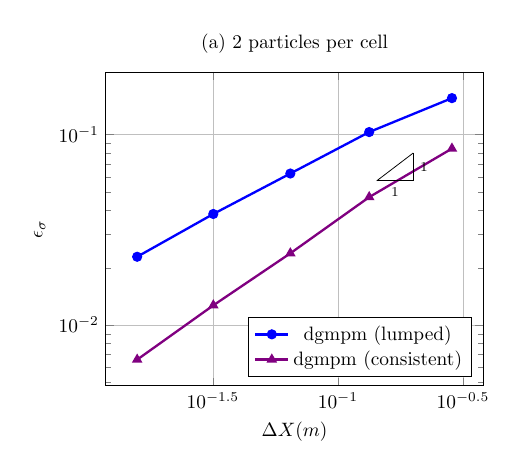
\begin{tikzpicture}[scale=0.7]
\begin{loglogaxis}[xlabel=$\Delta X (m)$,ylabel=$\epsilon_\sigma$,ymajorgrids=true,xmajorgrids=true,legend pos=south east,title={(a) 2 particles per cell}]
\addplot[Blue,very thick,mark=*] coordinates {(0.285714285714,0.155344401413) (0.133333333333,0.103056278416) (0.0645161290323,0.0624467155513) (0.031746031746,0.0383032357895) (0.0157480314961,0.0228383166886) };
\addlegendentry{dgmpm (lumped)}
\addplot[Purple,very thick,mark=triangle*] coordinates {(0.285714285714,0.0844046229439) (0.133333333333,0.0469432859143) (0.0645161290323,0.0238077178296) (0.031746031746,0.0126928564059) (0.0157480314961,0.0065867196308) };
\addlegendentry{dgmpm (consistent)}
\draw (axis cs:0.2,0.08) -- (axis cs:0.2/1.4,0.08/1.4);
\draw (axis cs:0.2,0.08) -- (axis cs:0.2,0.08/1.4) node [midway,right] {\scriptsize 1};
\draw (axis cs:0.2,0.08/1.4) -- (axis cs:0.2/1.4,0.08/1.4) node [midway,below] {\scriptsize 1};
\end{loglogaxis}
\end{tikzpicture}

        \end{column}
        \begin{column}{0.49\textwidth}
          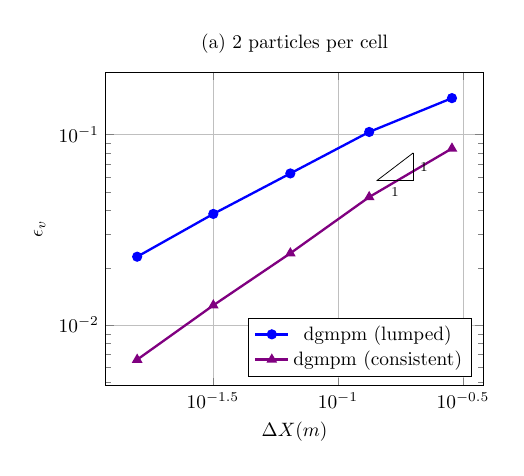
\begin{tikzpicture}[scale=0.7]
\begin{loglogaxis}[xlabel=$\Delta X (m)$,ylabel=$\epsilon_v$,ymajorgrids=true,xmajorgrids=true,legend pos=south east,title={(a) 2 particles per cell}]
\addplot[Blue,very thick,mark=*] coordinates {(0.285714285714,0.155081880585) (0.133333333333,0.103056265942) (0.0645161290323,0.0624467155504) (0.031746031746,0.0383032357895) (0.0157480314961,0.0228383166886) };
\addlegendentry{dgmpm (lumped)}
\addplot[Purple,very thick,mark=triangle*] coordinates {(0.285714285714,0.0844044636359) (0.133333333333,0.0469432859143) (0.0645161290323,0.0238077178296) (0.031746031746,0.0126928564059) (0.0157480314961,0.0065867196308) };
\addlegendentry{dgmpm (consistent)}
\draw (axis cs:0.2,0.08) -- (axis cs:0.2/1.4,0.08/1.4);
\draw (axis cs:0.2,0.08) -- (axis cs:0.2,0.08/1.4) node [midway,right] {\scriptsize 1};
\draw (axis cs:0.2,0.08/1.4) -- (axis cs:0.2/1.4,0.08/1.4) node [midway,below] {\scriptsize 1};
\end{loglogaxis}
\end{tikzpicture}

        \end{column}
      \end{columns}
    \end{block}
  \end{overprint}
\end{frame}

%%% Local Variables:
%%% mode: latex
%%% TeX-master: "../presentation"
%%% End:
